\documentclass[]{article}
\usepackage{lmodern}
\usepackage{amssymb,amsmath}
\usepackage{ifxetex,ifluatex}
\usepackage{fixltx2e} % provides \textsubscript
\ifnum 0\ifxetex 1\fi\ifluatex 1\fi=0 % if pdftex
  \usepackage[T1]{fontenc}
  \usepackage[utf8]{inputenc}
\else % if luatex or xelatex
  \ifxetex
    \usepackage{mathspec}
  \else
    \usepackage{fontspec}
  \fi
  \defaultfontfeatures{Ligatures=TeX,Scale=MatchLowercase}
\fi
% use upquote if available, for straight quotes in verbatim environments
\IfFileExists{upquote.sty}{\usepackage{upquote}}{}
% use microtype if available
\IfFileExists{microtype.sty}{%
\usepackage{microtype}
\UseMicrotypeSet[protrusion]{basicmath} % disable protrusion for tt fonts
}{}
\usepackage[margin=1in]{geometry}
\usepackage{hyperref}
\hypersetup{unicode=true,
            pdftitle={Lab 3 Report},
            pdfauthor={Priscilla Burity, Oscar Linares, Alissa Stover},
            pdfborder={0 0 0},
            breaklinks=true}
\urlstyle{same}  % don't use monospace font for urls
\usepackage{color}
\usepackage{fancyvrb}
\newcommand{\VerbBar}{|}
\newcommand{\VERB}{\Verb[commandchars=\\\{\}]}
\DefineVerbatimEnvironment{Highlighting}{Verbatim}{commandchars=\\\{\}}
% Add ',fontsize=\small' for more characters per line
\usepackage{framed}
\definecolor{shadecolor}{RGB}{248,248,248}
\newenvironment{Shaded}{\begin{snugshade}}{\end{snugshade}}
\newcommand{\AlertTok}[1]{\textcolor[rgb]{0.94,0.16,0.16}{#1}}
\newcommand{\AnnotationTok}[1]{\textcolor[rgb]{0.56,0.35,0.01}{\textbf{\textit{#1}}}}
\newcommand{\AttributeTok}[1]{\textcolor[rgb]{0.77,0.63,0.00}{#1}}
\newcommand{\BaseNTok}[1]{\textcolor[rgb]{0.00,0.00,0.81}{#1}}
\newcommand{\BuiltInTok}[1]{#1}
\newcommand{\CharTok}[1]{\textcolor[rgb]{0.31,0.60,0.02}{#1}}
\newcommand{\CommentTok}[1]{\textcolor[rgb]{0.56,0.35,0.01}{\textit{#1}}}
\newcommand{\CommentVarTok}[1]{\textcolor[rgb]{0.56,0.35,0.01}{\textbf{\textit{#1}}}}
\newcommand{\ConstantTok}[1]{\textcolor[rgb]{0.00,0.00,0.00}{#1}}
\newcommand{\ControlFlowTok}[1]{\textcolor[rgb]{0.13,0.29,0.53}{\textbf{#1}}}
\newcommand{\DataTypeTok}[1]{\textcolor[rgb]{0.13,0.29,0.53}{#1}}
\newcommand{\DecValTok}[1]{\textcolor[rgb]{0.00,0.00,0.81}{#1}}
\newcommand{\DocumentationTok}[1]{\textcolor[rgb]{0.56,0.35,0.01}{\textbf{\textit{#1}}}}
\newcommand{\ErrorTok}[1]{\textcolor[rgb]{0.64,0.00,0.00}{\textbf{#1}}}
\newcommand{\ExtensionTok}[1]{#1}
\newcommand{\FloatTok}[1]{\textcolor[rgb]{0.00,0.00,0.81}{#1}}
\newcommand{\FunctionTok}[1]{\textcolor[rgb]{0.00,0.00,0.00}{#1}}
\newcommand{\ImportTok}[1]{#1}
\newcommand{\InformationTok}[1]{\textcolor[rgb]{0.56,0.35,0.01}{\textbf{\textit{#1}}}}
\newcommand{\KeywordTok}[1]{\textcolor[rgb]{0.13,0.29,0.53}{\textbf{#1}}}
\newcommand{\NormalTok}[1]{#1}
\newcommand{\OperatorTok}[1]{\textcolor[rgb]{0.81,0.36,0.00}{\textbf{#1}}}
\newcommand{\OtherTok}[1]{\textcolor[rgb]{0.56,0.35,0.01}{#1}}
\newcommand{\PreprocessorTok}[1]{\textcolor[rgb]{0.56,0.35,0.01}{\textit{#1}}}
\newcommand{\RegionMarkerTok}[1]{#1}
\newcommand{\SpecialCharTok}[1]{\textcolor[rgb]{0.00,0.00,0.00}{#1}}
\newcommand{\SpecialStringTok}[1]{\textcolor[rgb]{0.31,0.60,0.02}{#1}}
\newcommand{\StringTok}[1]{\textcolor[rgb]{0.31,0.60,0.02}{#1}}
\newcommand{\VariableTok}[1]{\textcolor[rgb]{0.00,0.00,0.00}{#1}}
\newcommand{\VerbatimStringTok}[1]{\textcolor[rgb]{0.31,0.60,0.02}{#1}}
\newcommand{\WarningTok}[1]{\textcolor[rgb]{0.56,0.35,0.01}{\textbf{\textit{#1}}}}
\usepackage{longtable,booktabs}
\usepackage{graphicx,grffile}
\makeatletter
\def\maxwidth{\ifdim\Gin@nat@width>\linewidth\linewidth\else\Gin@nat@width\fi}
\def\maxheight{\ifdim\Gin@nat@height>\textheight\textheight\else\Gin@nat@height\fi}
\makeatother
% Scale images if necessary, so that they will not overflow the page
% margins by default, and it is still possible to overwrite the defaults
% using explicit options in \includegraphics[width, height, ...]{}
\setkeys{Gin}{width=\maxwidth,height=\maxheight,keepaspectratio}
\IfFileExists{parskip.sty}{%
\usepackage{parskip}
}{% else
\setlength{\parindent}{0pt}
\setlength{\parskip}{6pt plus 2pt minus 1pt}
}
\setlength{\emergencystretch}{3em}  % prevent overfull lines
\providecommand{\tightlist}{%
  \setlength{\itemsep}{0pt}\setlength{\parskip}{0pt}}
\setcounter{secnumdepth}{0}
% Redefines (sub)paragraphs to behave more like sections
\ifx\paragraph\undefined\else
\let\oldparagraph\paragraph
\renewcommand{\paragraph}[1]{\oldparagraph{#1}\mbox{}}
\fi
\ifx\subparagraph\undefined\else
\let\oldsubparagraph\subparagraph
\renewcommand{\subparagraph}[1]{\oldsubparagraph{#1}\mbox{}}
\fi

%%% Use protect on footnotes to avoid problems with footnotes in titles
\let\rmarkdownfootnote\footnote%
\def\footnote{\protect\rmarkdownfootnote}

%%% Change title format to be more compact
\usepackage{titling}

% Create subtitle command for use in maketitle
\providecommand{\subtitle}[1]{
  \posttitle{
    \begin{center}\large#1\end{center}
    }
}

\setlength{\droptitle}{-2em}

  \title{Lab 3 Report}
    \pretitle{\vspace{\droptitle}\centering\huge}
  \posttitle{\par}
    \author{Priscilla Burity, Oscar Linares, Alissa Stover}
    \preauthor{\centering\large\emph}
  \postauthor{\par}
      \predate{\centering\large\emph}
  \postdate{\par}
    \date{Due: 4/14/2020}


\begin{document}
\maketitle

{
\setcounter{tocdepth}{2}
\tableofcontents
}
\hypertarget{introduction}{%
\section{Introduction}\label{introduction}}

\textbf{Which policies are most promising in reducing crime rate: those
that target punishing crimes (criminal justice policy) or reducing the
need to commit crimes (economic policy)?}

To answer this question, we used a cross-section of data on crime
statistics and related factors (e.g., economic indicators) for a
selection of counties in North Carolina. These data were first used in a
study by Cornwell and Trumball, researchers from the University of
Georgia and West Virginia University (C. Cornwell and W. Trumball
(1994), ``Estimating the Economic Model of Crime with Panel Data,''
Review of Economics and Statistics 76, 360-366). Most of the data are
from 1987, except for some demographic variables from the 1980 Census.
Our task was to help a political campaign understand the determinants of
crime and to generate local policy suggestions to curb it. As such, we
focused on variables that can be influenced by policy.

We also included a range of contextual variables that control for local
characteristics influencing crime and the efficacy of these policies. In
contrast to our variables of main focus, these are generally not
actionable (e.g., demographic and geographic indicators).

The key assumption in our analysis is that all county attributes come
from from the same sample. For example, the demographic characteristics
from one county correspond to the same people who would commit crimes.
In other words, we don't have people committing crimes in one county but
living in another.

The data were limited in the following ways: (1) they only contained one
year of cross-sectional data, (2) there are important omitted variables,
and (3) they provide little variation in the distribution of policy
variables. Having data from one year alone means that the context of
that specific year is an uncontrolled factor. For example, one specific
event that could have affected both crime and economic variables was the
\href{https://en.wikipedia.org/wiki/Black_Monday_(1987)}{Black Monday
crash in October of that year}. Issues (2) and (3) made it difficult to
isolate the true effect of policies. Firstly, omitted variables like
unemployment would likely affect crime as well as other explanatory
variables. Secondly, variation in policies across counties is needed to
identify their impact on crime and some policies - such as as minimum
wage and tax levels - were similar across all counties in the 1980s.
Thus, in general, these issues limits the causal claims we can make.

That said, we produced a model that could help to guide policy decisions
aimed at reducing crime across these counties.

The main finding was that acting on crime deterrents within the criminal
justice system (like arrests and convictions) is important when it comes
to preventing crime. In fact, for a 10\% rise in the probability of
arrests and convictions individually, the reduction on crime rate hovers
between 4-7\% for arrests and between 3-5\% for convictions. This result
has a material practical significance.

Even though we could not find much support for the importance of
economic policy variables to prevent crimes, this could be due to this
dataset's lack of a good metric for this kind of policy.

\hypertarget{actionable-variables}{%
\subsection{Actionable Variables}\label{actionable-variables}}

\hypertarget{criminal-justice-policy}{%
\subsubsection{Criminal Justice Policy}\label{criminal-justice-policy}}

Many of these criminal justice policies are used as deterrents of crime,
with the assumption being that people will be less likely to commit
crimes because they will want to avoid the punishment.

The 3 variables below are dubbed ``probabilities''. However, this is a
misnomer as these variables are truly ratios. We interpret these as
measures of the assertiveness of the criminal justice system in a
county.

\hypertarget{probability-of-arrest}{%
\paragraph{Probability of arrest}\label{probability-of-arrest}}

If we find that the assertiveness of arrest is associated with crime
rate (i.e.~higher punishment is associated with lower crime), we may
consider stricter policies around police practice that encourage more
arrests.

\begin{itemize}
\tightlist
\item
  \texttt{prbarr}: number of arrests for every crime reported
\end{itemize}

\hypertarget{probability-of-conviction}{%
\paragraph{Probability of conviction}\label{probability-of-conviction}}

If we find that the assertiveness of conviction is associated with crime
rate (i.e.~higher conviction rates are associated with lower crime), we
may consider stricter policies around court practices so that more
arrests lead to convictions.

\begin{itemize}
\tightlist
\item
  \texttt{prbconv}: number of convictions for every arrest made
\end{itemize}

\hypertarget{probability-of-sentencing}{%
\paragraph{Probability of sentencing}\label{probability-of-sentencing}}

If we find that the assertiveness of sentencing is associated with crime
rate (i.e.~higher sentencing rates are associated with lower crime), we
may consider stricter policies around judicial practices so that more
convictions lead to sentencing.

A prison sentence depends on the severity of the crime and as such
counties with more severe crime would see elevated numbers for this
variable (and vice versa). Thus, this variable may be more limited in
its explanatory power than arrests and convictions and will not be a
prime candidate for our model.

\begin{itemize}
\tightlist
\item
  \texttt{prbpris}: number of prison sentences for every conviction
\end{itemize}

\hypertarget{severity-of-punishment}{%
\paragraph{Severity of punishment}\label{severity-of-punishment}}

If we find that the severity of punishment is associated with crime rate
(i.e.~greater severity is associated with lower crime), we may consider
stricter policies around judicial practices so that people receive more
severe punishments. Similarly to prison sentence rate, the length of
someone's sentence depends on the severity of the crime. Thus, this
variable may also be more limited in its explanatory power than arrests
and convictions and will not be a prime candidate for our model.

\begin{itemize}
\tightlist
\item
  \texttt{avgsen}: average sentence in days
\end{itemize}

\hypertarget{number-of-police-officers-per-capita}{%
\paragraph{Number of police officers per
capita}\label{number-of-police-officers-per-capita}}

The number of police officers per capita (\texttt{polpc}) is a very
intuitive example of crime deterrent, since in theory it increases the
likelihood of being caught in the act of the crime and it is also a
measure of the capacity of the State to enforce the law. However,
cross-sectional data limitations prevent us from understanding the
relationship between police officers per capita and crime rate because
the impact of increasing the number of police per capita might not be
realized in the same period. One can expect that counties with larger
crime rates in a year \emph{t} would consider it necessary to have a
larger number of police officers on the streets in year \emph{t}, which
can imply a positive correlation between presence of police and crime
rates that does not necessarily go one way in terms of causality.

As our job is to advise a policy maker, it is very important that we
feel safe about the causal interpretation of our findings. We need to
avoid potential reverse causality effects between independent and
dependent variables. Thus, in this exercise we opted not to include
police per capita as a candidate policy variable nor covariate.

\hypertarget{economic-policy}{%
\subsubsection{Economic Policy}\label{economic-policy}}

We used the wage variables to operationalize economic policy because
these variables could be reshaped with economic policy. For example, if
increased wages are found to be related significantly to crime, our
candidate could consider strategies such as raising the minimum wage in
an attempt to lower crime.

Additionally, empirical research, such as
\href{https://www.journals.uchicago.edu/doi/abs/10.1086/449290}{that
described in this paper}, suggests that increasing a worker's wage can
deter the worker from committing crimes. Completely omitting these
variables could introduce bias on the other estimated relationships.

The following are weekly wages in different sectors:

\begin{itemize}
\tightlist
\item
  \texttt{wcon}: construction
\item
  \texttt{wtuc}: transportation, utilities, communication
\item
  \texttt{wtrd}: wholesale and retail trade
\item
  \texttt{wfir}: finance, insurance, real estate
\item
  \texttt{wser}: services
\item
  \texttt{wmfg}: manufacturing
\item
  \texttt{wsta}: state employees
\item
  \texttt{wloc}: local government employees
\end{itemize}

The federal wage variable was grouped with other wages in much of our
exploratory data analyses for easier comparison; however, it is not
related to minimum wage policy but rather to cost of living. Federal
employee wages are controlled by the federal government and are
\href{https://www.opm.gov/policy-data-oversight/pay-leave/salaries-wages/fact-sheets/}{adjusted
for a locality's cost of living}. A relationship between federal wages
and crime could predict that changing the cost of living may affect
crime.

Policy recommendations that could be made from this variable are limited
by the fact that we are missing important economic variables such as
inequality. Raising the cost of living alone would not have the intended
effect on crime without a combined effort to address inequality. For
example, areas with high cost of living and high rates of inequality
would expect to see more crime, as those who are \emph{in need} would
find more reason to take from those who have \emph{more than they need}.

Although it may be complicated to interpret our quantification of the
relationship between crime and this variable, we imagine that omitting
this variable could introduce bias in other estimated relationships.
Thus, it is important to attempt to measure the relationship between
federal wages and crime to test the robustness of other variables.

\begin{itemize}
\tightlist
\item
  \texttt{wfed}: federal employees
\end{itemize}

The following variable represents tax revenue per capita, but does not
differentiate between different revenue streams (income, sales,
property, or businesses). Many taxes are set at the state and federal
level and so the level of variation at the county-level may be limited.
Since this variable could represent a mix of effects, the causal
relationship would be difficult to interpret but we included this
variable as an important covariate to test other relationships.

\begin{itemize}
\tightlist
\item
  \texttt{taxpc}: tax revenue per capita
\end{itemize}

\hypertarget{contextual-variables}{%
\subsection{Contextual Variables}\label{contextual-variables}}

The following variables describe county characteristics that provide
important information about how policies could work across different
contexts. Although they are not actionable, they strengthen our ability
to make causal inferences.

\hypertarget{types-of-crime}{%
\subsubsection{Types of Crime}\label{types-of-crime}}

If an area has mostly petty crimes, one would imagine that some of the
punishment (e.g., fines) could be less visible and perhaps less of a
deterrent than arresting people. This difference could change the
relationship between our crime policy variables and crime rate.

\begin{itemize}
\tightlist
\item
  \texttt{mix}: offense mix: face-to-face/other
\end{itemize}

\hypertarget{demographics}{%
\subsubsection{Demographics}\label{demographics}}

\hypertarget{urbanrural-dwellers}{%
\paragraph{Urban/rural dwellers}\label{urbanrural-dwellers}}

Higher density areas would see more interaction between people, which
could drive up crime. Also, social bonds and norms in small communities
could act as deterrents of crime.

\begin{itemize}
\tightlist
\item
  \texttt{density}: people per square mile
\end{itemize}

\hypertarget{minority-status}{%
\paragraph{Minority status}\label{minority-status}}

It is well known that people of minority status (compared to Caucasians)
are more likely to be involved in the criminal justice system (this
doesn't mean they actually commit more crimes, just that they are
arrested more often) and as such this is a key covariate in our
analysis.

\begin{itemize}
\tightlist
\item
  \texttt{pctmin80}: percent minority, 1980
\end{itemize}

\hypertarget{gender-age}{%
\paragraph{Gender \& Age}\label{gender-age}}

Young males are more likely to enter the criminal justice system; this
is another demographic variable that we would expect relates to crime.

\begin{itemize}
\tightlist
\item
  \texttt{pctymle}: percent young male, 1980
\end{itemize}

\hypertarget{geography}{%
\subsubsection{Geography}\label{geography}}

The following variables identifies a county's region within the state,
with the assumption that counties cluster geographically in terms of
culture and other characteristics we are not explicitly measuring.
Western North Carolina is along the Appalachian mountains and
qualitatively different from the rest of the state. For example,
\href{https://www.google.com/maps/search/universities+colleges+north+carolina/@35.6210094,-82.5051642,7z}{it
has fewer universities and colleges}.

\begin{itemize}
\tightlist
\item
  \texttt{west}: =1 if in western N.C.
\item
  \texttt{central}: =1 if in central N.C.
\item
  \texttt{urban}: =1 if in SMSA
\end{itemize}

\hypertarget{model-building-process}{%
\section{Model Building Process}\label{model-building-process}}

\hypertarget{data-cleaning-exploratory-data-analysis}{%
\subsection{Data Cleaning \& Exploratory Data
Analysis}\label{data-cleaning-exploratory-data-analysis}}

\begin{Shaded}
\begin{Highlighting}[]
\CommentTok{# import libraries }
\KeywordTok{library}\NormalTok{(tidyverse) }\CommentTok{# for data import, manipulation, viz}
\KeywordTok{library}\NormalTok{(corrplot) }\CommentTok{# for correlation matix}
\KeywordTok{library}\NormalTok{(stargazer) }\CommentTok{# visualize model fit}
\KeywordTok{library}\NormalTok{(skimr) }\CommentTok{# generate summary statistics}
\KeywordTok{library}\NormalTok{(car) }\CommentTok{# statistics }
\KeywordTok{library}\NormalTok{(lmtest) }\CommentTok{# linear modeling}
\KeywordTok{library}\NormalTok{(olsrr) }\CommentTok{# evaluating OLS regression }
\KeywordTok{library}\NormalTok{(sandwich) }\CommentTok{# correcting heteroskedasticity violation}
\KeywordTok{library}\NormalTok{(grid) }\CommentTok{# to arrange ggplot figures into a grid }
\KeywordTok{library}\NormalTok{(gridExtra) }\CommentTok{# to arrange ggplot figures into a grid }
\KeywordTok{library}\NormalTok{(wesanderson) }\CommentTok{# color palettes}
\end{Highlighting}
\end{Shaded}

\begin{Shaded}
\begin{Highlighting}[]
\CommentTok{# import data}
\NormalTok{data <-}\StringTok{ }\KeywordTok{read_csv}\NormalTok{(}\StringTok{"crime_v2.csv"}\NormalTok{, }\DataTypeTok{n_max =} \DecValTok{91}\NormalTok{)}
\end{Highlighting}
\end{Shaded}

\hypertarget{file-level-data-checks}{%
\paragraph{File-level data checks}\label{file-level-data-checks}}

We have 91 observations and 25 columns in the raw data. All 25 columns
were read in as numeric columns.

\begin{Shaded}
\begin{Highlighting}[]
\KeywordTok{print}\NormalTok{(}\KeywordTok{paste}\NormalTok{(}\StringTok{"Number of records:"}\NormalTok{, }\KeywordTok{dim}\NormalTok{(data)[}\DecValTok{1}\NormalTok{]))}
\end{Highlighting}
\end{Shaded}

\begin{verbatim}
## [1] "Number of records: 91"
\end{verbatim}

\begin{Shaded}
\begin{Highlighting}[]
\KeywordTok{print}\NormalTok{(}\KeywordTok{paste}\NormalTok{(}\StringTok{"Number of variables:"}\NormalTok{, }\KeywordTok{dim}\NormalTok{(data)[}\DecValTok{2}\NormalTok{]))}
\end{Highlighting}
\end{Shaded}

\begin{verbatim}
## [1] "Number of variables: 25"
\end{verbatim}

\hypertarget{the-where-when-of-these-data}{%
\subparagraph{The Where \& When of these
data}\label{the-where-when-of-these-data}}

We had 1 observation for each of the counties in the raw data, except
for county \#193. We noticed that these rows appear to be exact
duplicates.

\begin{Shaded}
\begin{Highlighting}[]
\NormalTok{data }\OperatorTok\StringTok{ }\KeywordTok{filter}\NormalTok{(county }\OperatorTok{==}\StringTok{ }\DecValTok{193}\NormalTok{)}
\end{Highlighting}
\end{Shaded}

\begin{verbatim}
## # A tibble: 2 x 25
##   county  year crmrte prbarr prbconv prbpris avgsen   polpc density taxpc
##    <dbl> <dbl>  <dbl>  <dbl>   <dbl>   <dbl>  <dbl>   <dbl>   <dbl> <dbl>
## 1    193    87 0.0235  0.266   0.589   0.423   5.86 0.00118   0.814  28.5
## 2    193    87 0.0235  0.266   0.589   0.423   5.86 0.00118   0.814  28.5
## # ... with 15 more variables: west <dbl>, central <dbl>, urban <dbl>,
## #   pctmin80 <dbl>, wcon <dbl>, wtuc <dbl>, wtrd <dbl>, wfir <dbl>,
## #   wser <dbl>, wmfg <dbl>, wfed <dbl>, wsta <dbl>, wloc <dbl>, mix <dbl>,
## #   pctymle <dbl>
\end{verbatim}

The attributes associated with each record led us to believe that the
\href{https://www.lib.ncsu.edu/gis/countfips}{county IDs are county FIPS
codes}. We supplement some of our data quality checks with internet
searches on counties according to their FIPS code, without assuming that
there is perfect alignment with the county IDs.

The \texttt{year} column is an expected constant (1987). We dropped this
column in future data processing steps.

\begin{Shaded}
\begin{Highlighting}[]
\KeywordTok{table}\NormalTok{(data}\OperatorTok{$}\NormalTok{year, }\DataTypeTok{useNA =} \StringTok{"always"}\NormalTok{)}
\end{Highlighting}
\end{Shaded}

\begin{verbatim}
## 
##   87 <NA> 
##   91    0
\end{verbatim}

We created a new data frame dropping superfluous columns (\texttt{year}
and \texttt{polpc}) and row (duplicate of county 193), ending with 90
rows and 24 numeric variables. Since we had one row per county, the
dataset appears to be missing information from 10 of the 100 counties in
North Carolina.

\begin{Shaded}
\begin{Highlighting}[]
\NormalTok{data2 <-}\StringTok{ }\NormalTok{data }\OperatorTok\StringTok{ }\KeywordTok{distinct}\NormalTok{() }\OperatorTok\StringTok{ }\KeywordTok{select}\NormalTok{(}\OperatorTok{-}\KeywordTok{c}\NormalTok{(}\StringTok{"year"}\NormalTok{, }\StringTok{"polpc"}\NormalTok{))}
\end{Highlighting}
\end{Shaded}

\hypertarget{missingness-data-validity}{%
\subparagraph{Missingness \& Data
Validity}\label{missingness-data-validity}}

We can see from the following table that we didn't have any data missing
from the raw file.

However, we spotted a few values that are extremely high based on
maximum values (p100). For example, one county has weekly wages in the
service sector reported to be \$2177 (almost 10x the median of \$253).

Note that \texttt{pctmin80} values are not in the {[}0,1{]} scale
despite being a percentage of total metric. The scale for this variable
does not match the other percentage metric in our data set
(\texttt{pctymle}) and was adjusted to facilitate coefficient
interpretation.

\begin{Shaded}
\begin{Highlighting}[]
\CommentTok{#generate skim table}
\NormalTok{data2_skim <-}\StringTok{ }\KeywordTok{skim}\NormalTok{(data2)}
\NormalTok{data2_skim}
\end{Highlighting}
\end{Shaded}

\begin{verbatim}
## Skim summary statistics
##  n obs: 90 
##  n variables: 23 
## 
## -- Variable type:numeric ----------------------------------------------------------------------------------------
##  variable missing complete  n    mean      sd         p0     p25     p50
##    avgsen       0       90 90   9.69    2.83      5.38     7.38    9.11 
##   central       0       90 90   0.38    0.49      0        0       0    
##    county       0       90 90 100.6    58.32      1       51.5   103    
##    crmrte       0       90 90   0.034   0.019     0.0055   0.021   0.03 
##   density       0       90 90   1.44    1.52  2e-05        0.55    0.98 
##       mix       0       90 90   0.13    0.082     0.02     0.081   0.1  
##  pctmin80       0       90 90  25.71   16.98      1.28    10.02   24.85 
##   pctymle       0       90 90   0.084   0.023     0.062    0.074   0.078
##    prbarr       0       90 90   0.3     0.14      0.093    0.2     0.27 
##   prbconv       0       90 90   0.55    0.35      0.068    0.34    0.45 
##   prbpris       0       90 90   0.41    0.081     0.15     0.36    0.42 
##     taxpc       0       90 90  38.16   13.11     25.69    30.73   34.92 
##     urban       0       90 90   0.089   0.29      0        0       0    
##      wcon       0       90 90 285.35   47.75    193.64   250.75  281.16 
##      west       0       90 90   0.24    0.43      0        0       0    
##      wfed       0       90 90 442.62   59.95    326.1    398.78  448.85 
##      wfir       0       90 90 321.62   54       170.94   285.56  317.13 
##      wloc       0       90 90 312.28   28.13    239.17   297.23  307.65 
##      wmfg       0       90 90 336.03   88.23    157.41   288.6   321.05 
##      wser       0       90 90 275.34  207.4     133.04   229.34  253.12 
##      wsta       0       90 90 357.74   43.29    258.33   329.27  358.4  
##      wtrd       0       90 90 210.92   33.87    154.21   190.71  202.99 
##      wtuc       0       90 90 410.91   77.36    187.62   374.33  404.78 
##      p75     p100     hist
##   11.47    20.7   ▆▇▅▅▂▁▁▁
##    1        1     ▇▁▁▁▁▁▁▅
##  150.5    197     ▇▆▇▇▆▇▇▇
##    0.04     0.099 ▆▇▇▃▂▁▁▁
##    1.57     8.83  ▇▃▁▁▁▁▁▁
##    0.15     0.47  ▃▇▂▁▁▁▁▁
##   38.18    64.35  ▇▅▅▅▆▃▁▂
##    0.084    0.25  ▇▁▁▁▁▁▁▁
##    0.34     1.09  ▆▇▃▁▁▁▁▁
##    0.59     2.12  ▃▇▂▁▁▁▁▁
##    0.46     0.6   ▁▁▂▅▇▇▂▁
##   41.01   119.76  ▇▃▁▁▁▁▁▁
##    0        1     ▇▁▁▁▁▁▁▁
##  314.98   436.77  ▂▇▇▇▅▃▁▁
##    0        1     ▇▁▁▁▁▁▁▂
##  478.26   597.95  ▃▅▅▇▆▃▂▁
##  342.63   509.47  ▁▁▅▇▃▁▁▁
##  328.78   388.09  ▁▁▃▇▅▂▁▁
##  359.89   646.85  ▁▃▇▅▁▁▁▁
##  277.65  2177.07  ▇▁▁▁▁▁▁▁
##  383.15   499.59  ▂▃▆▇▆▂▁▁
##  224.28   354.68  ▃▇▆▂▂▁▁▁
##  440.68   613.23  ▁▁▂▆▇▂▂▁
\end{verbatim}

\begin{Shaded}
\begin{Highlighting}[]
\CommentTok{# convert % minority variable}
\NormalTok{data2}\OperatorTok{$}\NormalTok{pctmin80 <-}\StringTok{ }\NormalTok{data2}\OperatorTok{$}\NormalTok{pctmin80 }\OperatorTok{*}\StringTok{ }\FloatTok{0.01}
\end{Highlighting}
\end{Shaded}

\begin{Shaded}
\begin{Highlighting}[]
\CommentTok{# save clean data file }
\KeywordTok{save}\NormalTok{(data2, }\DataTypeTok{file =} \StringTok{"data_clean.rda"}\NormalTok{)}
\end{Highlighting}
\end{Shaded}

\hypertarget{variable-level-data-checks-exploratory-data-analysis}{%
\subsection{Variable-level data checks \& Exploratory Data
Analysis}\label{variable-level-data-checks-exploratory-data-analysis}}

\hypertarget{dependent-variable-crime-rate}{%
\subsubsection{Dependent Variable: Crime
Rate}\label{dependent-variable-crime-rate}}

In Figure 1, we used a histogram to visualize the shape of
\texttt{crmrte}'s distribution and see that it is unimodal and
approximately normal (with a slight skew). Most values are between 0.02
- 0.04 with some to 0.10. We don't appear to have any spurious values.

\begin{Shaded}
\begin{Highlighting}[]
\KeywordTok{ggplot}\NormalTok{(data2, }\KeywordTok{aes}\NormalTok{(crmrte)) }\OperatorTok{+}
\StringTok{  }\KeywordTok{geom_histogram}\NormalTok{(}\DataTypeTok{bins =} \DecValTok{35}\NormalTok{, }\DataTypeTok{fill =} \StringTok{"seashell4"}\NormalTok{, }\DataTypeTok{color =} \StringTok{"grey28"}\NormalTok{) }\OperatorTok{+}
\StringTok{  }\KeywordTok{theme_minimal}\NormalTok{() }\OperatorTok{+}
\StringTok{  }\KeywordTok{xlab}\NormalTok{(}\StringTok{"Crime Rate"}\NormalTok{) }\OperatorTok{+}
\StringTok{  }\KeywordTok{ylab}\NormalTok{(}\StringTok{"Frequency"}\NormalTok{) }\OperatorTok{+}
\StringTok{  }\KeywordTok{ggtitle}\NormalTok{(}\StringTok{"Histogram of Dependent Variable: Crime Rate"}\NormalTok{)}
\end{Highlighting}
\end{Shaded}

\begin{figure}

{\centering 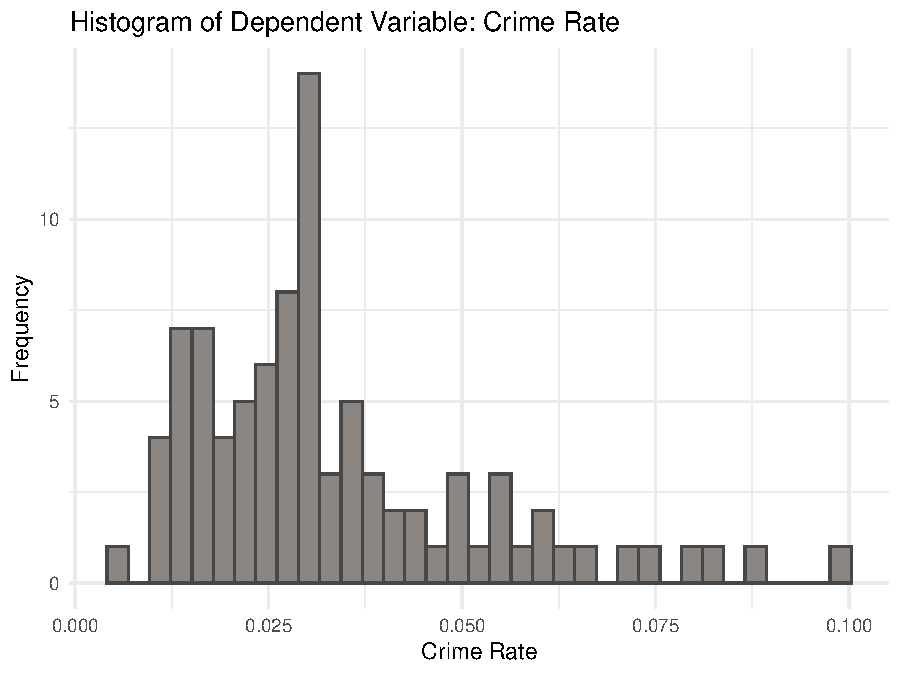
\includegraphics{lab_3_final_files/figure-latex/unnamed-chunk-10-1} 

}

\caption{Figure 1}\label{fig:unnamed-chunk-10}
\end{figure}

\hypertarget{independent-variables}{%
\subsubsection{Independent Variables}\label{independent-variables}}

\hypertarget{actionable-variables-1}{%
\paragraph{Actionable Variables}\label{actionable-variables-1}}

\hypertarget{criminal-justice-policy-1}{%
\subparagraph{Criminal Justice Policy}\label{criminal-justice-policy-1}}

From our violin plots in Figure 2, we see that we have different
distributions for the 3 core criminal justice policy variables
(\texttt{prbarr}, \texttt{prbconv}, \texttt{prbpris}), but that they
have a similar shape (unimodal with different levels of skew). The
embedded boxplots reveal some extreme values for conviction rate, with
multiple counties having a rate above 1. These values imply that for
each arrest, there could be multiple convictions - one county has over 2
convictions for every arrest. Only 1 county has more than 1 arrest per
crime committed - most counties in fact put someone under arrest for
about one-quarter of crimes. When it comes to sentencing, counties show
a much lower spread and cluster around 1 conviction, resulting in a
prison sentence for every other conviction.

\begin{Shaded}
\begin{Highlighting}[]
\CommentTok{# format data for subplots }
\NormalTok{data_cj_long <-}\StringTok{ }\NormalTok{data2 }\OperatorTok\StringTok{ }\KeywordTok{select}\NormalTok{(prbarr, prbconv, prbpris) }\OperatorTok
\StringTok{  }\KeywordTok{gather}\NormalTok{(}\DataTypeTok{key =}\NormalTok{ var, }\DataTypeTok{value =}\NormalTok{ value)}

\CommentTok{# convert to factor for subplot labelling }
\NormalTok{data_cj_long}\OperatorTok{$}\NormalTok{var <-}\StringTok{ }\KeywordTok{factor}\NormalTok{(data_cj_long}\OperatorTok{$}\NormalTok{var, }\DataTypeTok{labels =} \KeywordTok{c}\NormalTok{(}\StringTok{"Prob Arrest"}\NormalTok{, }\StringTok{"Prob Convicted"}\NormalTok{, }\StringTok{"Prob Sentenced"}\NormalTok{))}
\end{Highlighting}
\end{Shaded}

\begin{Shaded}
\begin{Highlighting}[]
\CommentTok{# plot violin/boxplot }
\KeywordTok{ggplot}\NormalTok{(data_cj_long, }\KeywordTok{aes}\NormalTok{(}\DataTypeTok{x =}\NormalTok{ var, }\DataTypeTok{y =}\NormalTok{ value, }\DataTypeTok{fill =}\NormalTok{ var)) }\OperatorTok{+}
\StringTok{  }\KeywordTok{geom_violin}\NormalTok{(}\DataTypeTok{fill =} \StringTok{"thistle3"}\NormalTok{, }\DataTypeTok{color =} \StringTok{"grey28"}\NormalTok{) }\OperatorTok{+}\StringTok{ }
\StringTok{  }\KeywordTok{geom_boxplot}\NormalTok{(}\DataTypeTok{width=}\FloatTok{0.1}\NormalTok{, }\DataTypeTok{fill =} \StringTok{"white"}\NormalTok{) }\OperatorTok{+}\StringTok{ }
\StringTok{  }\KeywordTok{theme_minimal}\NormalTok{() }\OperatorTok{+}
\StringTok{  }\KeywordTok{xlab}\NormalTok{(}\StringTok{""}\NormalTok{) }\OperatorTok{+}
\StringTok{  }\KeywordTok{ylab}\NormalTok{(}\StringTok{"Ratio"}\NormalTok{) }\OperatorTok{+}\StringTok{ }
\StringTok{  }\KeywordTok{ggtitle}\NormalTok{(}\StringTok{"Criminal Justice Policy Variables: Assertiveness Variables"}\NormalTok{)}
\end{Highlighting}
\end{Shaded}

\begin{figure}

{\centering 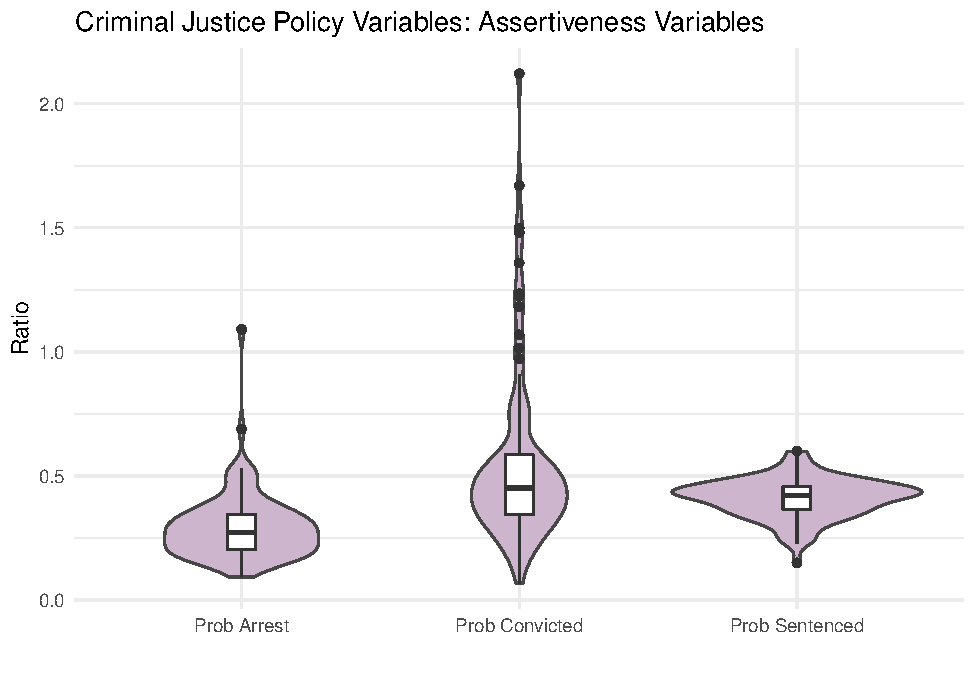
\includegraphics{lab_3_final_files/figure-latex/unnamed-chunk-12-1} 

}

\caption{Figure 2}\label{fig:unnamed-chunk-12}
\end{figure}

\emph{Which county had the lowest conviction rate?} This is County \#11,
which has a very high arrest rate given its conviction rate. However, we
could not spot anything that would indicate this erroneous or irrelevant
data.

\begin{Shaded}
\begin{Highlighting}[]
\NormalTok{data2 }\OperatorTok\StringTok{ }\KeywordTok{filter}\NormalTok{(prbconv }\OperatorTok{==}\StringTok{ }\KeywordTok{min}\NormalTok{(prbconv)) }\OperatorTok\StringTok{ }\KeywordTok{select}\NormalTok{(county, prbarr, prbconv, prbpris, avgsen, pctmin80)}
\end{Highlighting}
\end{Shaded}

\begin{verbatim}
## # A tibble: 1 x 6
##   county prbarr prbconv prbpris avgsen pctmin80
##    <dbl>  <dbl>   <dbl>   <dbl>  <dbl>    <dbl>
## 1     11  0.525  0.0684     0.5     13   0.0154
\end{verbatim}

\emph{Which county had the highest conviction rate?} This is a county in
central North Carolina. It also has the highest percentage of
minorities.

\begin{Shaded}
\begin{Highlighting}[]
\NormalTok{data2 }\OperatorTok\StringTok{ }\KeywordTok{filter}\NormalTok{(prbconv }\OperatorTok{==}\StringTok{ }\KeywordTok{max}\NormalTok{(prbconv)) }\OperatorTok\StringTok{ }\KeywordTok{select}\NormalTok{(county, prbarr, prbconv, prbpris, avgsen, pctmin80)}
\end{Highlighting}
\end{Shaded}

\begin{verbatim}
## # A tibble: 1 x 6
##   county prbarr prbconv prbpris avgsen pctmin80
##    <dbl>  <dbl>   <dbl>   <dbl>  <dbl>    <dbl>
## 1    185  0.195    2.12   0.443   5.38    0.643
\end{verbatim}

The fact that the conviction rate is so high seems odd for county \#185.
We can see from Figure 3 that the other measures of assertiveness (for
arrest and sentencing) seem close to their medians.

\begin{Shaded}
\begin{Highlighting}[]
\NormalTok{data_prb <-}\StringTok{ }\NormalTok{data2 }\OperatorTok\StringTok{ }\KeywordTok{as_tibble}\NormalTok{() }\OperatorTok\StringTok{ }\KeywordTok{select}\NormalTok{(prbarr, prbconv, prbpris) }\OperatorTok\StringTok{ }\KeywordTok{summarise_all}\NormalTok{(median) }\OperatorTok\StringTok{ }
\StringTok{  }\KeywordTok{gather}\NormalTok{(var, value) }\OperatorTok\StringTok{ }\KeywordTok{mutate}\NormalTok{(}\DataTypeTok{Group =} \StringTok{"Median"}\NormalTok{)}

\NormalTok{data_ep_long <-}\StringTok{ }\NormalTok{data2 }\OperatorTok\StringTok{ }
\StringTok{  }\KeywordTok{select}\NormalTok{(wcon, wtuc, wtrd, wfir, wser, wmfg, wfed, wsta, wloc) }\OperatorTok
\StringTok{  }\KeywordTok{gather}\NormalTok{(}\DataTypeTok{key =}\NormalTok{ var, }\DataTypeTok{value =}\NormalTok{ value)}

\NormalTok{prb_}\DecValTok{185}\NormalTok{ <-}\StringTok{ }\NormalTok{data2 }\OperatorTok\StringTok{  }\KeywordTok{as_tibble}\NormalTok{() }\OperatorTok\StringTok{ }\KeywordTok{filter}\NormalTok{(county }\OperatorTok{==}\StringTok{ }\DecValTok{185}\NormalTok{) }\OperatorTok\StringTok{ }\KeywordTok{select}\NormalTok{(prbarr, prbconv, prbpris) }\OperatorTok\StringTok{ }
\StringTok{  }\KeywordTok{gather}\NormalTok{(var, value) }\OperatorTok\StringTok{ }\KeywordTok{mutate}\NormalTok{(}\DataTypeTok{Group =} \StringTok{"County #185"}\NormalTok{)}

\NormalTok{prbs <-}\StringTok{ }\KeywordTok{bind_rows}\NormalTok{(data_prb, prb_}\DecValTok{185}\NormalTok{)}

\KeywordTok{ggplot}\NormalTok{(}\DataTypeTok{data =}\NormalTok{ prbs, }\KeywordTok{aes}\NormalTok{(}\DataTypeTok{x =}\NormalTok{ var, }\DataTypeTok{y =}\NormalTok{ value, }\DataTypeTok{color =}\NormalTok{ Group)) }\OperatorTok{+}\StringTok{ }
\StringTok{  }\KeywordTok{geom_point}\NormalTok{(}\DataTypeTok{size =} \DecValTok{4}\NormalTok{, }\DataTypeTok{alpha =} \FloatTok{.7}\NormalTok{) }\OperatorTok{+}
\StringTok{  }\KeywordTok{xlab}\NormalTok{(}\StringTok{'Criminal Justice Assertiveness Category'}\NormalTok{) }\OperatorTok{+}
\StringTok{  }\KeywordTok{ylab}\NormalTok{(}\StringTok{'Assertiveness'}\NormalTok{) }\OperatorTok{+}
\StringTok{  }\KeywordTok{theme_minimal}\NormalTok{() }\OperatorTok{+}
\StringTok{  }\KeywordTok{ggtitle}\NormalTok{(}\StringTok{"Criminal Justice Assertiveness: County 185 vs. Median"}\NormalTok{)}
\end{Highlighting}
\end{Shaded}

\begin{figure}

{\centering 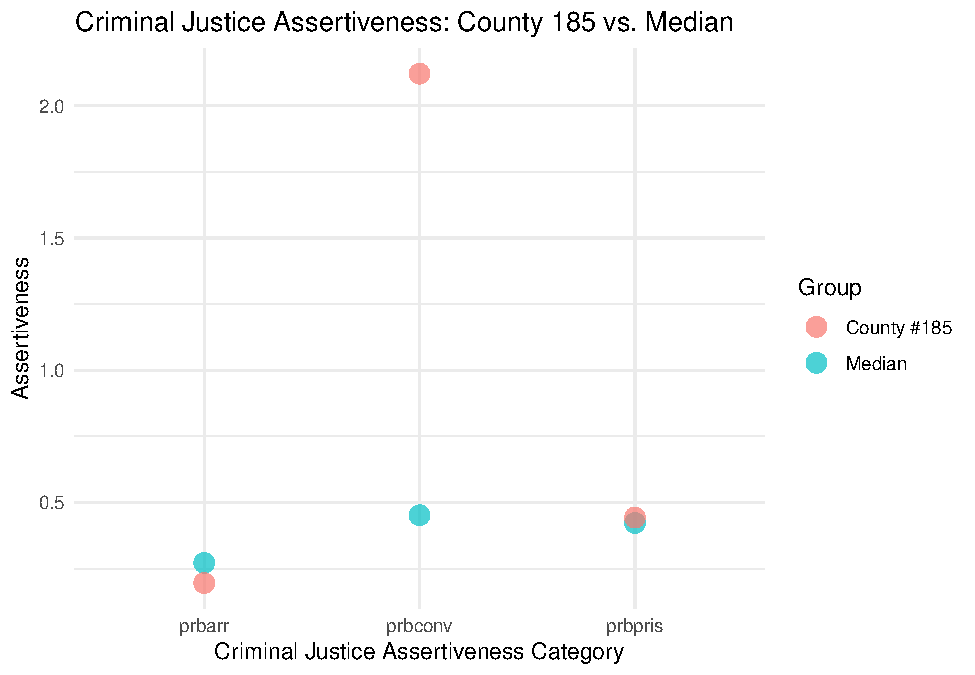
\includegraphics{lab_3_final_files/figure-latex/unnamed-chunk-15-1} 

}

\caption{Figure 3}\label{fig:unnamed-chunk-15}
\end{figure}

According to the FIPS codes, \#185 stands for Warren County.
\href{https://en.wikipedia.org/wiki/Warren_County_PCB_Landfill}{During
the 1980s, its citizens conducted a series of demonstrations against a
newly built landfill}, which led to multiple arrests and convictions
associated with disobedience (not crime). This was an extraordinary
event outside the process of interest, so we will remove this county.

We see from Figure 4 that average sentence length follows an
approximately normal distribution with one extremely high value, which
corresponds to Madison County (according to the FIPS code). This western
county is home to the state's oldest jail,
\href{https://mountainx.com/news/murky-future-for-madisons-historic-jailhouse/}{still
in operation in 1987}. The fact that this county is in one of the less
prosperous areas of the USA and home to this jail could explain its
average sentence length. We retain this outlier in the data since it
probably doesn't indicate spurious data and would be an interesting edge
case to study.

\begin{Shaded}
\begin{Highlighting}[]
\KeywordTok{ggplot}\NormalTok{(data2, }\KeywordTok{aes}\NormalTok{(avgsen)) }\OperatorTok{+}
\StringTok{  }\KeywordTok{geom_histogram}\NormalTok{(}\DataTypeTok{binwidth =} \DecValTok{1}\NormalTok{, }\DataTypeTok{fill =} \StringTok{"thistle3"}\NormalTok{, }\DataTypeTok{color =} \StringTok{"grey28"}\NormalTok{) }\OperatorTok{+}
\StringTok{  }\KeywordTok{theme_minimal}\NormalTok{() }\OperatorTok{+}
\StringTok{  }\KeywordTok{xlab}\NormalTok{(}\StringTok{"Days of Imprisonment"}\NormalTok{) }\OperatorTok{+}
\StringTok{  }\KeywordTok{ylab}\NormalTok{(}\StringTok{"Frequency"}\NormalTok{) }\OperatorTok{+}
\StringTok{  }\KeywordTok{ggtitle}\NormalTok{(}\StringTok{"Criminal Justice Policy Variables: Assertiveness Variables"}\NormalTok{)}
\end{Highlighting}
\end{Shaded}

\begin{figure}

{\centering 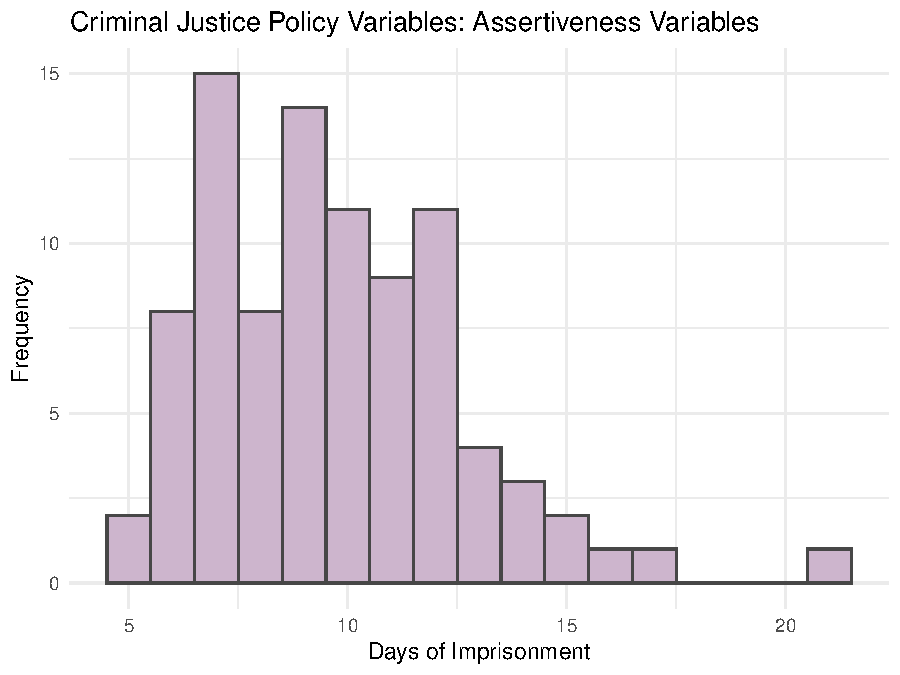
\includegraphics{lab_3_final_files/figure-latex/unnamed-chunk-16-1} 

}

\caption{Figure 4}\label{fig:unnamed-chunk-16}
\end{figure}

\begin{Shaded}
\begin{Highlighting}[]
\NormalTok{data2 }\OperatorTok\StringTok{ }\KeywordTok{filter}\NormalTok{(avgsen }\OperatorTok{==}\StringTok{ }\KeywordTok{max}\NormalTok{(avgsen)) }\OperatorTok\StringTok{ }\KeywordTok{select}\NormalTok{(county, avgsen, west, urban)}
\end{Highlighting}
\end{Shaded}

\begin{verbatim}
## # A tibble: 1 x 4
##   county avgsen  west urban
##    <dbl>  <dbl> <dbl> <dbl>
## 1    115   20.7     1     0
\end{verbatim}

\hypertarget{economic-policy-1}{%
\subparagraph{Economic Policy}\label{economic-policy-1}}

Minimum wage is one of the few economic factors that state/local
politicians can change. In North Carolina in 1987, the minimum hourly
wage was \$3.35 (\$134 per week, given a 40 hour week).

In Figure 5, we plot weekly wage by sector with a red vertical line
indicating this minimum weekly wage.

The violin plots with embedded boxplots make it clear that Wholesale \&
Retail Trade wages are closest to the minimum wage - suggesting that
wages in this sector are most under the influence of minimum wage
policy. The next sector that would be most influenced is Services. Note
that wages in the Services industry may be an inaccurate measure of
income because many of its workers make additional and often unreported
income through tips. Thus, \texttt{wtrd} would be more sensitive to a
minimum wage policy.

Another aspect of wage that our candidate could influence are state and
local employee wages. Raising the wages of government employees could
increase the quality of social services, reducing crime. Conversely, it
could cut into budgets for other crime-cutting efforts and may increase
crime. We included these in our models in order to test this policy but
implementation may be challenging.

\begin{Shaded}
\begin{Highlighting}[]
\CommentTok{# format data for subplots }
\NormalTok{data_ep_long <-}\StringTok{ }\NormalTok{data2 }\OperatorTok\StringTok{ }
\StringTok{  }\KeywordTok{select}\NormalTok{(wcon, wtuc, wtrd, wfir, wser, wmfg, wfed, wsta, wloc) }\OperatorTok
\StringTok{  }\KeywordTok{gather}\NormalTok{(}\DataTypeTok{key =}\NormalTok{ var, }\DataTypeTok{value =}\NormalTok{ value)}
\CommentTok{# convert to factor for better labeling }
\NormalTok{data_ep_long}\OperatorTok{$}\NormalTok{var <-}\StringTok{ }\KeywordTok{factor}\NormalTok{(data_ep_long}\OperatorTok{$}\NormalTok{var,}
                           \DataTypeTok{levels =} \KeywordTok{c}\NormalTok{(}\StringTok{"wcon"}\NormalTok{, }\StringTok{"wtuc"}\NormalTok{, }\StringTok{"wtrd"}\NormalTok{, }\StringTok{"wfir"}\NormalTok{,}
                                      \StringTok{"wser"}\NormalTok{, }\StringTok{"wmfg"}\NormalTok{, }\StringTok{"wfed"}\NormalTok{, }\StringTok{"wsta"}\NormalTok{, }\StringTok{"wloc"}\NormalTok{),}
                           \DataTypeTok{labels =} \KeywordTok{c}\NormalTok{(}\StringTok{"Construction"}\NormalTok{, }
                                      \StringTok{"Utilities/Transport"}\NormalTok{, }
                                      \StringTok{"Wholesale & Retail Trade"}\NormalTok{,}
                                      \StringTok{"Finance/Insurance/Real Estate"}\NormalTok{,}
                                      \StringTok{"Services"}\NormalTok{,}
                                      \StringTok{"Manufacturing"}\NormalTok{,}
                                      \StringTok{"Federal Emp"}\NormalTok{,}
                                      \StringTok{"State Emp"}\NormalTok{,}
                                      \StringTok{"Local/State Emp"}\NormalTok{))}
\end{Highlighting}
\end{Shaded}

\begin{Shaded}
\begin{Highlighting}[]
\CommentTok{# plot violin & boxplot subplots }
\KeywordTok{ggplot}\NormalTok{(data_ep_long, }\KeywordTok{aes}\NormalTok{(}\DataTypeTok{x =}\NormalTok{ var, }\DataTypeTok{y =}\NormalTok{ value)) }\OperatorTok{+}
\StringTok{  }\KeywordTok{geom_violin}\NormalTok{(}\DataTypeTok{fill =} \StringTok{"lightseagreen"}\NormalTok{) }\OperatorTok{+}\StringTok{ }
\StringTok{  }\KeywordTok{geom_boxplot}\NormalTok{(}\DataTypeTok{width=}\FloatTok{0.1}\NormalTok{) }\OperatorTok{+}
\StringTok{  }\KeywordTok{coord_flip}\NormalTok{() }\OperatorTok{+}\StringTok{ }
\StringTok{  }\KeywordTok{theme_minimal}\NormalTok{() }\OperatorTok{+}
\StringTok{  }\KeywordTok{xlab}\NormalTok{(}\StringTok{""}\NormalTok{) }\OperatorTok{+}\StringTok{ }
\StringTok{  }\KeywordTok{ylab}\NormalTok{(}\StringTok{"Weekly Wage"}\NormalTok{) }\OperatorTok{+}
\StringTok{  }\KeywordTok{ggtitle}\NormalTok{(}\StringTok{"Economic Variables: Wages"}\NormalTok{)}\OperatorTok{+}
\StringTok{  }\KeywordTok{geom_hline}\NormalTok{(}\KeywordTok{aes}\NormalTok{(}\DataTypeTok{yintercept =} \DecValTok{134}\NormalTok{, }\DataTypeTok{color =} \StringTok{"red"}\NormalTok{)) }\OperatorTok{+}
\StringTok{  }\KeywordTok{theme}\NormalTok{(}\DataTypeTok{legend.position =} \StringTok{"none"}\NormalTok{)}
\end{Highlighting}
\end{Shaded}

\begin{figure}

{\centering 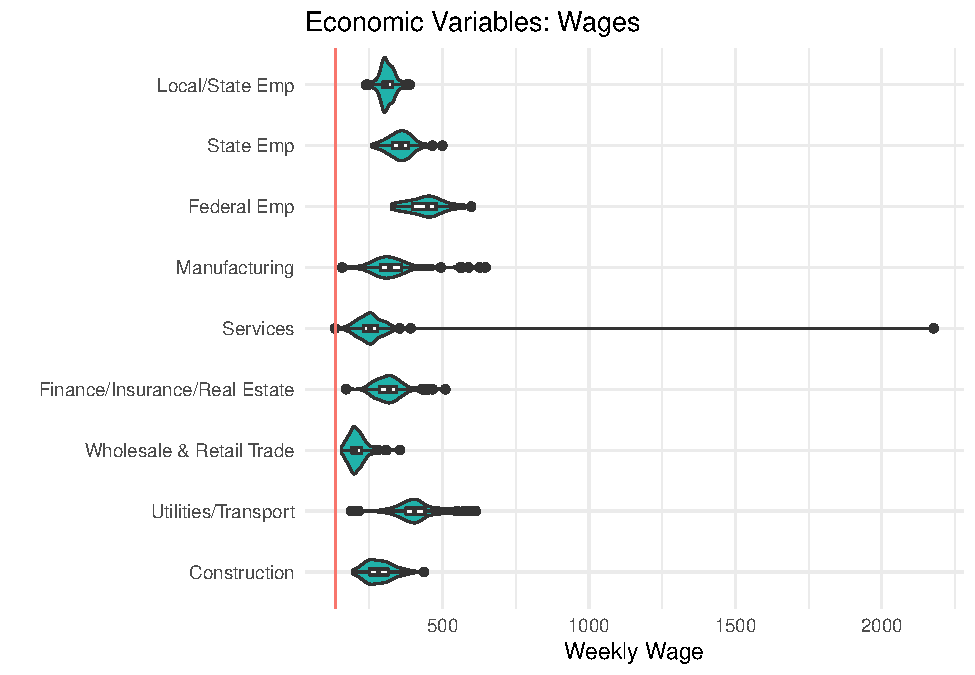
\includegraphics{lab_3_final_files/figure-latex/unnamed-chunk-19-1} 

}

\caption{Figure 5}\label{fig:unnamed-chunk-19}
\end{figure}

Another variable influenced by economic policy is tax revenue per
capita. Figure 6 demonstrates that the distribution of \texttt{taxpc} is
skewed. This distribution coupled with the fact that \texttt{taxpc} is
measured in dollars makes the variable a top candidate for a log
transformation.

\begin{Shaded}
\begin{Highlighting}[]
\CommentTok{# plot histogram & boxplot}
\KeywordTok{ggplot}\NormalTok{(data2, }\KeywordTok{aes}\NormalTok{(taxpc)) }\OperatorTok{+}
\StringTok{  }\KeywordTok{geom_histogram}\NormalTok{(}\DataTypeTok{binwidth =} \DecValTok{2}\NormalTok{, }\DataTypeTok{fill =} \StringTok{"lightseagreen"}\NormalTok{, }\DataTypeTok{color =} \StringTok{"grey28"}\NormalTok{) }\OperatorTok{+}
\StringTok{  }\KeywordTok{theme_minimal}\NormalTok{() }\OperatorTok{+}
\StringTok{  }\KeywordTok{xlab}\NormalTok{(}\StringTok{"Tax Revenue Per Capita"}\NormalTok{) }\OperatorTok{+}
\StringTok{  }\KeywordTok{ylab}\NormalTok{(}\StringTok{"Frequency"}\NormalTok{) }\OperatorTok{+}
\StringTok{  }\KeywordTok{ggtitle}\NormalTok{(}\StringTok{"Economic Variables: Tax Revenue Per Capita"}\NormalTok{)}
\end{Highlighting}
\end{Shaded}

\begin{figure}

{\centering 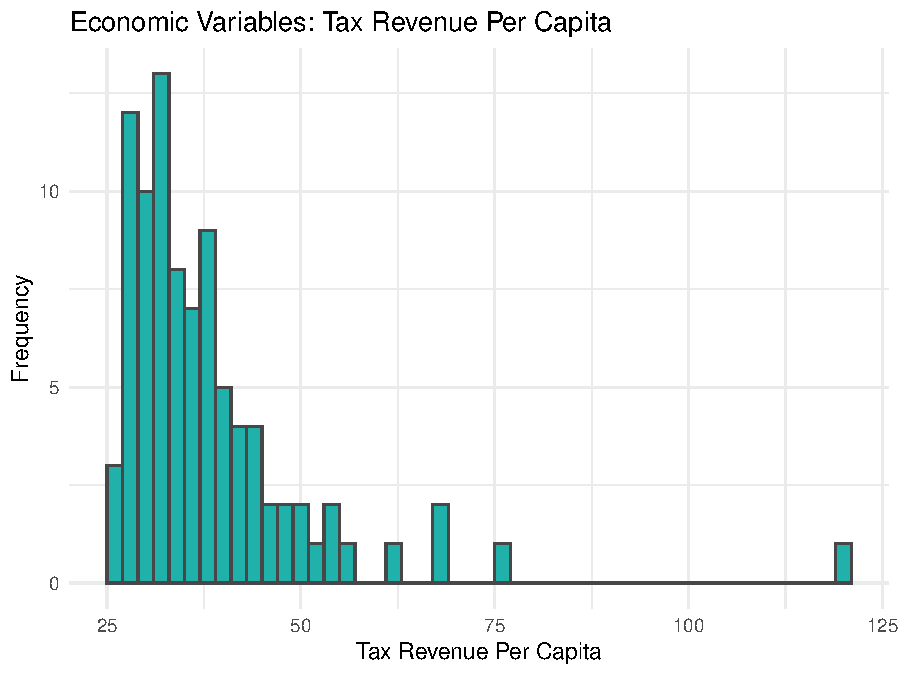
\includegraphics{lab_3_final_files/figure-latex/unnamed-chunk-20-1} 

}

\caption{Figure 6}\label{fig:unnamed-chunk-20}
\end{figure}

We appear to have an extreme value at \$119.76, which is for county
\#55. This is likely Dare County according to its FIPS code, a small
island that is a popular vacation spot.

One would expect that counties with high tax revenue also have high
wages of their populace. We checked the wages of this county against the
median and noticed that many were \emph{below or close to} the median.
This pattern (shown in Figure 7) could be explained by the fact that in
small touristy counties, an important share of taxes results from
tourism activities of non-residents, which boosts the region's tax
revenue per local citizen. Given that this row probably does not have a
data quality issue, we retained it.

\begin{Shaded}
\begin{Highlighting}[]
\CommentTok{# reformat data for plotting}
\NormalTok{data_tax <-}\StringTok{ }\NormalTok{data2 }\OperatorTok\StringTok{ }\KeywordTok{as_tibble}\NormalTok{() }\OperatorTok\StringTok{ }\KeywordTok{select}\NormalTok{(taxpc, wcon, wtuc, wtrd, wfir, wser, wmfg, wfed, wsta, wloc) }\OperatorTok\StringTok{ }\KeywordTok{summarise_all}\NormalTok{(median) }\OperatorTok\StringTok{ }
\StringTok{  }\KeywordTok{gather}\NormalTok{(var, value) }\OperatorTok\StringTok{ }\KeywordTok{mutate}\NormalTok{(}\DataTypeTok{Group =} \StringTok{"Median"}\NormalTok{)}
\NormalTok{taxes_}\DecValTok{55}\NormalTok{ <-}\StringTok{ }\NormalTok{data2 }\OperatorTok\StringTok{  }\KeywordTok{as_tibble}\NormalTok{() }\OperatorTok\StringTok{ }\KeywordTok{filter}\NormalTok{(county }\OperatorTok{==}\StringTok{ }\DecValTok{55}\NormalTok{) }\OperatorTok\StringTok{ }\KeywordTok{select}\NormalTok{(taxpc, wcon, wtuc, wtrd, wfir, wser, wmfg, wfed, wsta, wloc) }\OperatorTok\StringTok{ }
\StringTok{  }\KeywordTok{gather}\NormalTok{(var, value)}\OperatorTok\StringTok{ }\KeywordTok{mutate}\NormalTok{(}\DataTypeTok{Group =} \StringTok{"County #55"}\NormalTok{)}
\NormalTok{taxes <-}\StringTok{ }\KeywordTok{bind_rows}\NormalTok{(data_tax, taxes_}\DecValTok{55}\NormalTok{)}

\CommentTok{# plot}
\KeywordTok{ggplot}\NormalTok{(}\DataTypeTok{data =}\NormalTok{ taxes, }\KeywordTok{aes}\NormalTok{(}\DataTypeTok{x =}\NormalTok{ var, }\DataTypeTok{y =}\NormalTok{ value, }\DataTypeTok{color =}\NormalTok{ Group)) }\OperatorTok{+}\StringTok{ }
\StringTok{  }\KeywordTok{geom_point}\NormalTok{(}\DataTypeTok{size =} \DecValTok{4}\NormalTok{, }\DataTypeTok{alpha =} \FloatTok{.7}\NormalTok{) }\OperatorTok{+}
\StringTok{  }\KeywordTok{xlab}\NormalTok{(}\StringTok{'Category'}\NormalTok{) }\OperatorTok{+}
\StringTok{  }\KeywordTok{ylab}\NormalTok{(}\StringTok{'$'}\NormalTok{) }\OperatorTok{+}
\StringTok{  }\KeywordTok{theme_minimal}\NormalTok{() }\OperatorTok{+}
\StringTok{  }\KeywordTok{ggtitle}\NormalTok{(}\StringTok{"Tax Revenue and Wages: County 55 vs. Median"}\NormalTok{)}
\end{Highlighting}
\end{Shaded}

\begin{figure}

{\centering 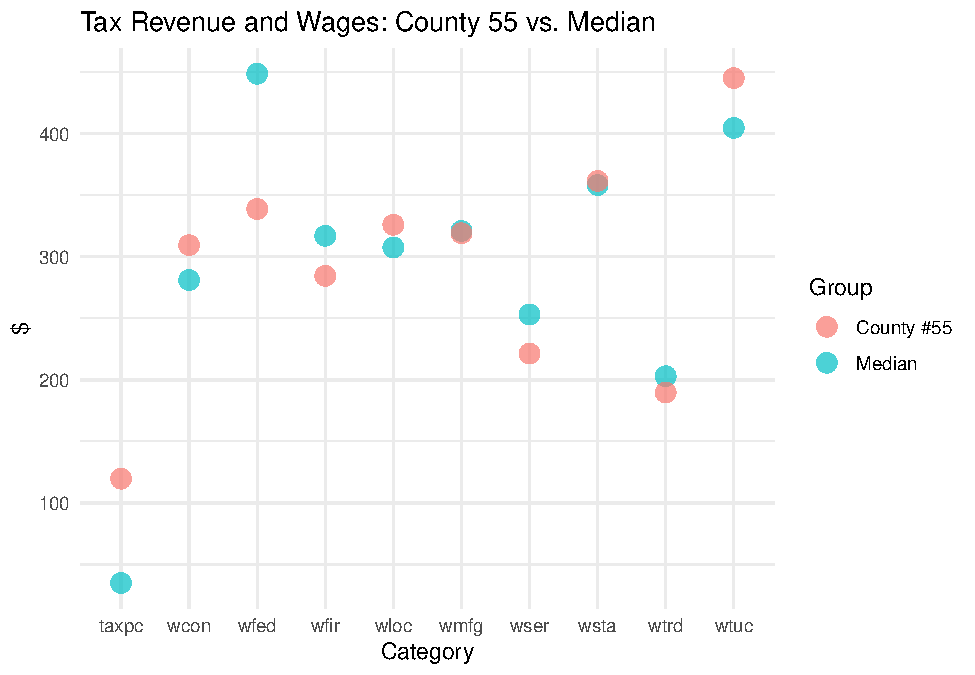
\includegraphics{lab_3_final_files/figure-latex/unnamed-chunk-21-1} 

}

\caption{Figure 7}\label{fig:unnamed-chunk-21}
\end{figure}

\hypertarget{contextual-variables-1}{%
\paragraph{Contextual Variables}\label{contextual-variables-1}}

Figure 8 reveals that the distributions for \texttt{mix},
\texttt{density} and \texttt{pctymle} approximate a normal distribution
but the that of \texttt{pctmin80} approximates a uniform distribution.
Minorities seem to be present in most counties in similar proportions.

\begin{Shaded}
\begin{Highlighting}[]
\CommentTok{# hist}
\NormalTok{p5 <-}\StringTok{ }\KeywordTok{ggplot}\NormalTok{(data2, }\KeywordTok{aes}\NormalTok{(mix)) }\OperatorTok{+}
\StringTok{  }\KeywordTok{geom_histogram}\NormalTok{(}\DataTypeTok{bins =} \DecValTok{35}\NormalTok{, }\DataTypeTok{color =} \StringTok{"grey28"}\NormalTok{, }\DataTypeTok{fill =} \KeywordTok{wes_palette}\NormalTok{(}\StringTok{"BottleRocket2"}\NormalTok{, }\DataTypeTok{n =} \DecValTok{1}\NormalTok{)) }\OperatorTok{+}
\StringTok{  }\KeywordTok{theme_minimal}\NormalTok{() }\OperatorTok{+}
\StringTok{  }\KeywordTok{ggtitle}\NormalTok{(}\StringTok{"Mix of Offense Types"}\NormalTok{) }\OperatorTok{+}
\StringTok{  }\KeywordTok{xlab}\NormalTok{(}\StringTok{"offense mix: face-to-face/other"}\NormalTok{)}

\NormalTok{p7 <-}\StringTok{ }\KeywordTok{ggplot}\NormalTok{(data2, }\KeywordTok{aes}\NormalTok{(density)) }\OperatorTok{+}
\StringTok{  }\KeywordTok{geom_histogram}\NormalTok{(}\DataTypeTok{bins =} \DecValTok{35}\NormalTok{, }\DataTypeTok{color =} \StringTok{"grey28"}\NormalTok{, }\DataTypeTok{fill =} \KeywordTok{wes_palette}\NormalTok{(}\StringTok{"BottleRocket2"}\NormalTok{, }\DataTypeTok{n =} \DecValTok{1}\NormalTok{)) }\OperatorTok{+}
\StringTok{  }\KeywordTok{theme_minimal}\NormalTok{() }\OperatorTok{+}
\StringTok{  }\KeywordTok{xlab}\NormalTok{(}\StringTok{"Density"}\NormalTok{) }\OperatorTok{+}
\StringTok{  }\KeywordTok{ylab}\NormalTok{(}\StringTok{"Count"}\NormalTok{) }\OperatorTok{+}
\StringTok{  }\KeywordTok{ggtitle}\NormalTok{(}\StringTok{"Population Density"}\NormalTok{)}

\NormalTok{p9 <-}\StringTok{ }\KeywordTok{ggplot}\NormalTok{(data2, }\KeywordTok{aes}\NormalTok{(pctmin80)) }\OperatorTok{+}
\StringTok{  }\KeywordTok{geom_histogram}\NormalTok{(}\DataTypeTok{bins =} \DecValTok{25}\NormalTok{, }\DataTypeTok{color =} \StringTok{"grey28"}\NormalTok{, }\DataTypeTok{fill =} \KeywordTok{wes_palette}\NormalTok{(}\StringTok{"BottleRocket2"}\NormalTok{, }\DataTypeTok{n =} \DecValTok{1}\NormalTok{)) }\OperatorTok{+}
\StringTok{  }\KeywordTok{theme_minimal}\NormalTok{() }\OperatorTok{+}
\StringTok{  }\KeywordTok{xlab}\NormalTok{(}\StringTok{"% Minority"}\NormalTok{) }\OperatorTok{+}
\StringTok{  }\KeywordTok{ylab}\NormalTok{(}\StringTok{"Count"}\NormalTok{) }\OperatorTok{+}
\StringTok{  }\KeywordTok{ggtitle}\NormalTok{(}\StringTok{"Percentage Minority (1980)"}\NormalTok{)}


\NormalTok{p11 <-}\StringTok{ }\KeywordTok{ggplot}\NormalTok{(data2, }\KeywordTok{aes}\NormalTok{(pctymle)) }\OperatorTok{+}
\StringTok{  }\KeywordTok{geom_histogram}\NormalTok{(}\DataTypeTok{bins =} \DecValTok{25}\NormalTok{, }\DataTypeTok{color =} \StringTok{"grey28"}\NormalTok{, }\DataTypeTok{fill =} \KeywordTok{wes_palette}\NormalTok{(}\StringTok{"BottleRocket2"}\NormalTok{, }\DataTypeTok{n =} \DecValTok{1}\NormalTok{)) }\OperatorTok{+}
\StringTok{  }\KeywordTok{theme_minimal}\NormalTok{() }\OperatorTok{+}
\StringTok{  }\KeywordTok{xlab}\NormalTok{(}\StringTok{"% Young Males"}\NormalTok{) }\OperatorTok{+}
\StringTok{  }\KeywordTok{ylab}\NormalTok{(}\StringTok{"Count"}\NormalTok{) }\OperatorTok{+}
\StringTok{  }\KeywordTok{ggtitle}\NormalTok{(}\StringTok{"Percentage Young Male (1980)"}\NormalTok{)}


\KeywordTok{grid.arrange}\NormalTok{(p5, p9, p7, p11, }\DataTypeTok{ncol =} \DecValTok{2}\NormalTok{, }\DataTypeTok{nrow =} \DecValTok{2}\NormalTok{, }\DataTypeTok{top =} \StringTok{"Contextual Variables"}\NormalTok{)}
\end{Highlighting}
\end{Shaded}

\begin{figure}

{\centering 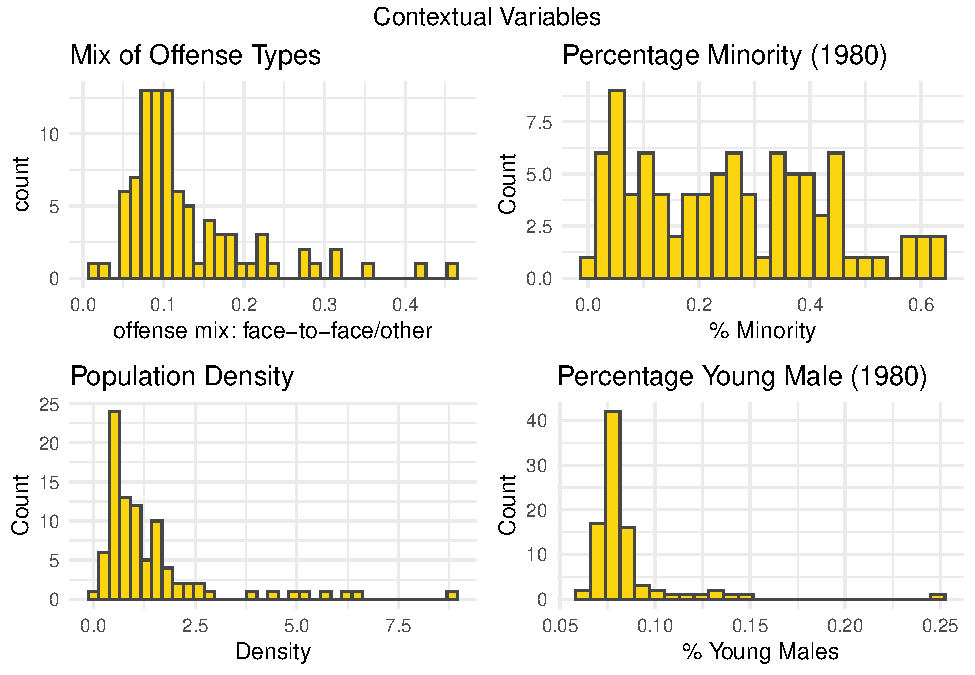
\includegraphics{lab_3_final_files/figure-latex/unnamed-chunk-22-1} 

}

\caption{Figure 8}\label{fig:unnamed-chunk-22}
\end{figure}

County \#119 has the highest density. This county probably is
Mecklenburg County, home to city of Charlotte (the state capital and one
of the most populated cities).

\begin{Shaded}
\begin{Highlighting}[]
\NormalTok{data2 }\OperatorTok\StringTok{ }\KeywordTok{filter}\NormalTok{(density }\OperatorTok{==}\StringTok{ }\KeywordTok{max}\NormalTok{(density)) }\OperatorTok\StringTok{ }\KeywordTok{select}\NormalTok{(county, density, central, urban)}
\end{Highlighting}
\end{Shaded}

\begin{verbatim}
## # A tibble: 1 x 4
##   county density central urban
##    <dbl>   <dbl>   <dbl> <dbl>
## 1    119    8.83       1     1
\end{verbatim}

The smallest density county would correspond to Swain County, a very
rural county in the Western part of the state. It straddles two national
parks/forests, which would explain why it has such low density.

\begin{Shaded}
\begin{Highlighting}[]
\NormalTok{data2 }\OperatorTok\StringTok{ }\KeywordTok{filter}\NormalTok{(density }\OperatorTok{==}\StringTok{ }\KeywordTok{min}\NormalTok{(density)) }\OperatorTok\StringTok{ }\KeywordTok{select}\NormalTok{(county, density, west, urban)}
\end{Highlighting}
\end{Shaded}

\begin{verbatim}
## # A tibble: 1 x 4
##   county   density  west urban
##    <dbl>     <dbl> <dbl> <dbl>
## 1    173 0.0000203     1     0
\end{verbatim}

We retained these rows, which don't have data quality issues and may be
edge cases of interest.

County \#133 (Onslow County based on FIPS code) is the main outlier for
\texttt{pctymle}. The deviation in percent of young males could be due
to Camp Lejeune, a marine corps base. Most recruits are young males and
so this base would impact the the county's share of young males,
especially if its population is small. As recruits would most likely not
commit crimes, this could interfere in our expected positive
relationship between the percent of young males and crime. However, this
is not the only county in North Carolina with a military base, so we
will keep this observation and monitor the estimated coefficient of
\texttt{pctymle} in our crime model.

\begin{Shaded}
\begin{Highlighting}[]
\NormalTok{data2 }\OperatorTok\StringTok{ }\KeywordTok{filter}\NormalTok{(pctymle }\OperatorTok{==}\StringTok{ }\KeywordTok{max}\NormalTok{(pctymle)) }\OperatorTok\StringTok{ }\KeywordTok{select}\NormalTok{(county, pctymle)}
\end{Highlighting}
\end{Shaded}

\begin{verbatim}
## # A tibble: 1 x 2
##   county pctymle
##    <dbl>   <dbl>
## 1    133   0.249
\end{verbatim}

\hypertarget{geography-1}{%
\subparagraph{Geography}\label{geography-1}}

We were given 3 variables to track geography. These are dummy variables
that code for west versus central versus east and urban versus rural.

The majority of North Carolina's population in 1987 was located in the
Central and Eastern parts of the state. Approximately one-quarter of the
population was in Western counties. Almost 90\% of North Carolina's
inhabitants lived in a rural area.

\begin{Shaded}
\begin{Highlighting}[]
\CommentTok{# create new east variable}
\NormalTok{geo_supp <-}\StringTok{ }\NormalTok{data2 }\OperatorTok\StringTok{ }\KeywordTok{mutate}\NormalTok{(}\DataTypeTok{east =} \KeywordTok{ifelse}\NormalTok{(west }\OperatorTok{==}\StringTok{ }\DecValTok{0} \OperatorTok{&}\StringTok{ }\NormalTok{central }\OperatorTok{==}\StringTok{ }\DecValTok{0}\NormalTok{, }\DecValTok{1}\NormalTok{, }\DecValTok{0}\NormalTok{), }\DataTypeTok{rural =} \KeywordTok{ifelse}\NormalTok{(urban }\OperatorTok{==}\StringTok{ }\DecValTok{0}\NormalTok{, }\DecValTok{1}\NormalTok{, }\DecValTok{0}\NormalTok{))}
\end{Highlighting}
\end{Shaded}

\begin{Shaded}
\begin{Highlighting}[]
\NormalTok{geo_pop_tbl <-}\StringTok{ }\KeywordTok{bind_cols}\NormalTok{(}\StringTok{"Location"}\NormalTok{ =}\StringTok{ }\KeywordTok{c}\NormalTok{(}\StringTok{"East"}\NormalTok{, }\StringTok{"Central"}\NormalTok{, }\StringTok{"West"}\NormalTok{),}
          \StringTok{"% of Population"}\NormalTok{ =}\StringTok{ }\KeywordTok{c}\NormalTok{(}\KeywordTok{round}\NormalTok{(}\DecValTok{100}\OperatorTok{*}\KeywordTok{sum}\NormalTok{(geo_supp}\OperatorTok{$}\NormalTok{east)}\OperatorTok{/}\DecValTok{90}\NormalTok{, }\DecValTok{2}\NormalTok{),}
                                    \KeywordTok{round}\NormalTok{(}\DecValTok{100}\OperatorTok{*}\KeywordTok{sum}\NormalTok{(geo_supp}\OperatorTok{$}\NormalTok{central)}\OperatorTok{/}\DecValTok{90}\NormalTok{, }\DecValTok{2}\NormalTok{),}
                                    \KeywordTok{round}\NormalTok{(}\DecValTok{100}\OperatorTok{*}\KeywordTok{sum}\NormalTok{(geo_supp}\OperatorTok{$}\NormalTok{west)}\OperatorTok{/}\DecValTok{90}\NormalTok{, }\DecValTok{2}\NormalTok{)))}

\NormalTok{type_pop_tbl <-}\StringTok{ }\KeywordTok{bind_cols}\NormalTok{(}\StringTok{"Type"}\NormalTok{ =}\StringTok{ }\KeywordTok{c}\NormalTok{(}\StringTok{"Urban"}\NormalTok{, }\StringTok{"Rural"}\NormalTok{),}
          \StringTok{"% of Population"}\NormalTok{ =}\StringTok{ }\KeywordTok{c}\NormalTok{(}\KeywordTok{round}\NormalTok{(}\DecValTok{100}\OperatorTok{*}\KeywordTok{sum}\NormalTok{(geo_supp}\OperatorTok{$}\NormalTok{urban)}\OperatorTok{/}\DecValTok{90}\NormalTok{, }\DecValTok{2}\NormalTok{),}
                                \KeywordTok{round}\NormalTok{(}\DecValTok{100}\OperatorTok{*}\KeywordTok{sum}\NormalTok{(geo_supp}\OperatorTok{$}\NormalTok{rural)}\OperatorTok{/}\DecValTok{90}\NormalTok{, }\DecValTok{2}\NormalTok{)))}
\NormalTok{knitr}\OperatorTok{::}\KeywordTok{kable}\NormalTok{(geo_pop_tbl)}
\end{Highlighting}
\end{Shaded}

\begin{longtable}[]{@{}lr@{}}
\toprule
Location & \% of Population\tabularnewline
\midrule
\endhead
East & 38.89\tabularnewline
Central & 37.78\tabularnewline
West & 24.44\tabularnewline
\bottomrule
\end{longtable}

\begin{Shaded}
\begin{Highlighting}[]
\NormalTok{knitr}\OperatorTok{::}\KeywordTok{kable}\NormalTok{(type_pop_tbl)}
\end{Highlighting}
\end{Shaded}

\begin{longtable}[]{@{}lr@{}}
\toprule
Type & \% of Population\tabularnewline
\midrule
\endhead
Urban & 8.89\tabularnewline
Rural & 91.11\tabularnewline
\bottomrule
\end{longtable}

Figure 9 demonstrates that the vast number of counties are rural across
central, western, and eastern counties. Central counties have the
largest share of urban geographies.

\begin{Shaded}
\begin{Highlighting}[]
\CommentTok{# reformat data for plotting}
\NormalTok{geo_long <-}\StringTok{ }\NormalTok{geo_supp }\OperatorTok
\StringTok{  }\KeywordTok{mutate_at}\NormalTok{(}\KeywordTok{vars}\NormalTok{(west, central, east, rural, urban), }\OperatorTok{~}\StringTok{ }\KeywordTok{ifelse}\NormalTok{(. }\OperatorTok{==}\StringTok{ }\DecValTok{0}\NormalTok{, }\OtherTok{NA}\NormalTok{, .)) }\OperatorTok
\StringTok{  }\KeywordTok{gather}\NormalTok{(}\StringTok{"location"}\NormalTok{, }\StringTok{"present1"}\NormalTok{, west, central, east, }\DataTypeTok{na.rm =} \OtherTok{TRUE}\NormalTok{) }\OperatorTok
\StringTok{  }\KeywordTok{gather}\NormalTok{(}\StringTok{"type"}\NormalTok{, }\StringTok{"present2"}\NormalTok{, rural, urban, }\DataTypeTok{na.rm =} \OtherTok{TRUE}\NormalTok{) }\OperatorTok
\StringTok{  }\KeywordTok{select}\NormalTok{(}\OperatorTok{-}\NormalTok{present1, }\OperatorTok{-}\NormalTok{present2)}
\end{Highlighting}
\end{Shaded}

\begin{Shaded}
\begin{Highlighting}[]
\CommentTok{# plot barplots}
\KeywordTok{ggplot}\NormalTok{(geo_long, }\KeywordTok{aes}\NormalTok{(}\DataTypeTok{x =}\NormalTok{ location, }\DataTypeTok{fill =}\NormalTok{ type)) }\OperatorTok{+}
\StringTok{  }\KeywordTok{geom_bar}\NormalTok{(}\DataTypeTok{position =} \StringTok{"fill"}\NormalTok{) }\OperatorTok{+}
\StringTok{  }\KeywordTok{scale_fill_manual}\NormalTok{(}\DataTypeTok{values =} \KeywordTok{wes_palette}\NormalTok{(}\StringTok{"GrandBudapest1"}\NormalTok{, }\DataTypeTok{n =} \DecValTok{3}\NormalTok{)) }\OperatorTok{+}\StringTok{ }
\StringTok{  }\KeywordTok{theme_minimal}\NormalTok{() }\OperatorTok{+}
\StringTok{  }\KeywordTok{ggtitle}\NormalTok{(}\StringTok{"Contextual Variables: Geography"}\NormalTok{) }\OperatorTok{+}
\StringTok{  }\KeywordTok{xlab}\NormalTok{(}\StringTok{""}\NormalTok{)}
\end{Highlighting}
\end{Shaded}

\begin{figure}

{\centering 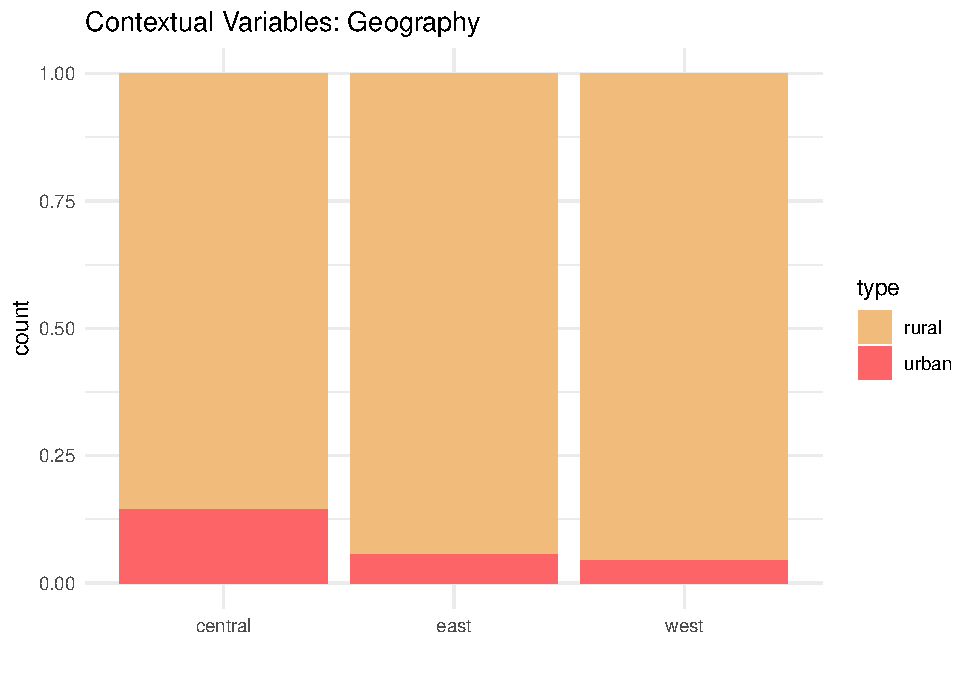
\includegraphics{lab_3_final_files/figure-latex/unnamed-chunk-29-1} 

}

\caption{Figure 9}\label{fig:unnamed-chunk-29}
\end{figure}

\hypertarget{relationships-between-variables}{%
\subsubsection{Relationships between
Variables}\label{relationships-between-variables}}

\begin{Shaded}
\begin{Highlighting}[]
\CommentTok{# remove row with erroneous values (#185) before investigating relationships }
\NormalTok{data2 <-}\StringTok{ }\NormalTok{data2 }\OperatorTok\StringTok{ }\KeywordTok{filter}\NormalTok{(county }\OperatorTok{!=}\StringTok{ }\DecValTok{185}\NormalTok{)}
\KeywordTok{print}\NormalTok{(}\KeywordTok{paste}\NormalTok{(}\StringTok{"Number of records:"}\NormalTok{, }\KeywordTok{dim}\NormalTok{(data2)[}\DecValTok{1}\NormalTok{]))}
\end{Highlighting}
\end{Shaded}

\begin{verbatim}
## [1] "Number of records: 89"
\end{verbatim}

Figure 10 is a correlation matrix of all of our variables, using
Spearman's due to the fact that not all variables follow a normal
distribution.

As expected, \texttt{prbarr} and \texttt{prbconv} showed a negative
correlation with \texttt{crmrte}. However, \texttt{prbpris} and
\texttt{avgsen} did not show a strong correlation with \texttt{cmrte}.
The fact that in general the number of imprisonments is low likely
weakens the relationship between \texttt{prbpris} and \texttt{cmrte}.
Also, given that most crimes committed are petty crimes with relatively
low sentence lengths, average sentence length might not be a strong
deterrent of crimes.

Additionally, \texttt{mix} did not seem to have a strong correlation
with \texttt{cmrte}. The values of \texttt{mix} were very low,
indicating that face-to-face crimes are almost non-existent across
counties. Thus, the low variability of \texttt{mix} does not allow for a
material relationship between it and crime rate.

Wages were mostly positively correlated with crime, opposite our
prediction. This unexpected direction could be explained in part by the
strong positive relationship between the wage variables and
\texttt{density} and between \texttt{crmrte} and \texttt{density}.
Usually, the bigger the city, the higher the wages but also the higher
the crime rate. This unexpected relationship could also be due to our
points above about inequality - if inequality is positively correlated
with both to crime and average wages, it could be a hidden factor that
is impacting this relationship. This pattern bolsters our decision to
\emph{not} include the wage variables in early models; it is crucial to
include additional controls when we do include them.

As expected, population density had a strong positive relationship with
crime rate. It was also positively correlated with other geographical
variables. For example, \texttt{urban} and \texttt{density} were
positively correlated because cities will have higher density. During
our analysis, we paid special attention to these strongly correlated
variables as they could increase the variance of models' residuals if
they are cast as independent variables in the same equation.

All wages as well as \texttt{taxpc} were positively correlated to each
other. This behavior was expected as wages and taxable income are both
determined by analogous economic factors. Similarly to the above, we
needed to pay close attention to the joint impact of including multiple
variables that are highly correlated in models.

\begin{Shaded}
\begin{Highlighting}[]
\CommentTok{# omit county to create correlation matrix }
\NormalTok{data_corr <-}\StringTok{ }\NormalTok{data2 }\OperatorTok\StringTok{ }\KeywordTok{select}\NormalTok{(}\OperatorTok{-}\NormalTok{county) }
\CommentTok{# create matrix of correlations}
\NormalTok{matrix_corr <-}\StringTok{ }\KeywordTok{round}\NormalTok{(}\KeywordTok{cor}\NormalTok{(data_corr, }\DataTypeTok{method =} \StringTok{"spearman"}\NormalTok{), }\DecValTok{1}\NormalTok{)}
\end{Highlighting}
\end{Shaded}

\begin{Shaded}
\begin{Highlighting}[]
\CommentTok{# visualize correlation matrix }
\KeywordTok{corrplot}\NormalTok{(matrix_corr, }\DataTypeTok{type =} \StringTok{"lower"}\NormalTok{, }\DataTypeTok{method =} \StringTok{"ellipse"}\NormalTok{, }\DataTypeTok{order =} \StringTok{"alphabet"}\NormalTok{)}
\end{Highlighting}
\end{Shaded}

\begin{figure}

{\centering 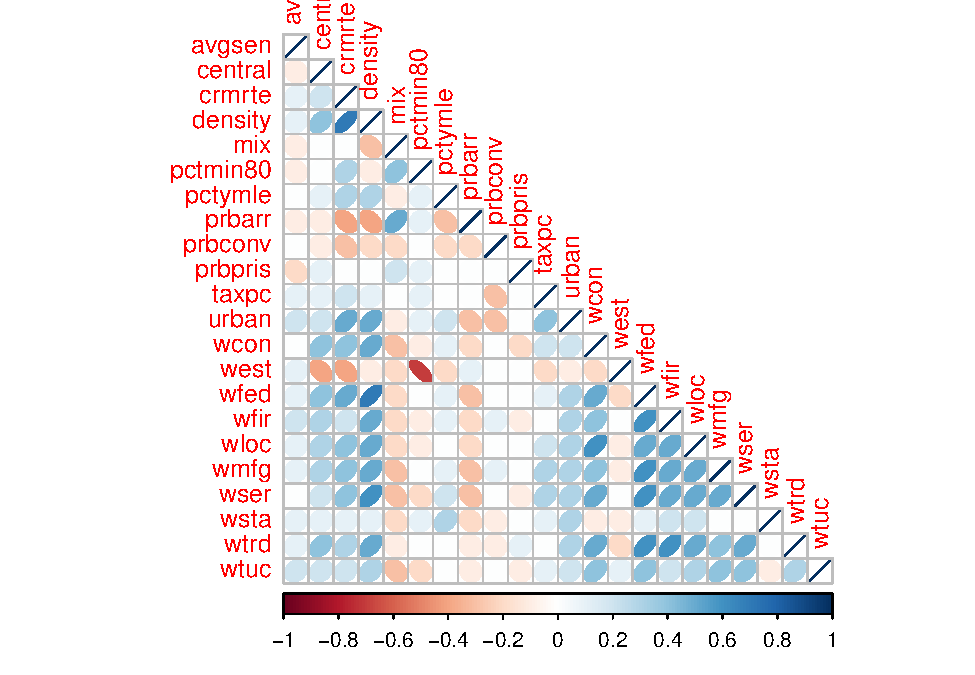
\includegraphics{lab_3_final_files/figure-latex/unnamed-chunk-32-1} 

}

\caption{Figure 10}\label{fig:unnamed-chunk-32}
\end{figure}

\hypertarget{model-results}{%
\subsection{Model Results}\label{model-results}}

In order select the optimal model in a certain range of model
specification options, we rely on information criteria. Two popular IC
are AIC (Akaike information criterion) and and BIC (Bayesian information
criterion). AIC and BIC for a model is usually written in the form
\(-2logL + kp\), where \(L\) is the likelihood function, \(p\) is the
number of parameters in the model, and \(k\) is \(2\) for AIC and
\(log(n)\) for BIC (\(n\)=number of observations). Despite subtle
theoretical differences, their only difference in practice is the size
of the penalty: BIC penalizes model complexity more heavily. To maintain
parsimony of our models, we opted to use BIC for model selection.

\hypertarget{model-set-1}{%
\subsubsection{Model set \#1}\label{model-set-1}}

For our first model, we aimed to evaluate the relationship between crime
policy and crime. We expected that more assertive crime policies will be
associated with lower crime rates.

We used the following independent variables:

\begin{enumerate}
\def\labelenumi{(\arabic{enumi})}
\item
  log(\texttt{prbarr})
\item
  log(\texttt{prbconv})
\item
  log(\texttt{prbpris})
\item
  log(\texttt{avg\_sen})
\end{enumerate}

\hypertarget{data-transformations}{%
\paragraph{Data Transformations}\label{data-transformations}}

We log transformed crime policy measures and \texttt{crmrte} to improve
our model fit and interpretability. With the log-log specification, the
coefficients of the criminal justice system variables can be interpreted
as the expected relative change in crime rate given a relative change in
assertiveness of the criminal justice system.

\hypertarget{discussion}{%
\paragraph{Discussion}\label{discussion}}

In the previous section, we found that \texttt{prbarr} and
\texttt{prbconv} had a strong negative correlation with \texttt{crmrte}
but \texttt{prbpris} and \texttt{avgsen} did not. With that in mind, in
the table below we compare the output of a model featuring only arrest
and conviction rates with the output of a model featuring all the crime
policy variables.

\begin{Shaded}
\begin{Highlighting}[]
\CommentTok{# create models}
\NormalTok{mod1_}\DecValTok{1}\NormalTok{ <-}\StringTok{ }\KeywordTok{lm}\NormalTok{(}\KeywordTok{log}\NormalTok{(crmrte) }\OperatorTok{~}\StringTok{ }\KeywordTok{log}\NormalTok{(prbarr) }\OperatorTok{+}\StringTok{ }\KeywordTok{log}\NormalTok{(prbconv) }\OperatorTok{+}\StringTok{ }\KeywordTok{log}\NormalTok{(prbpris) }\OperatorTok{+}\StringTok{ }\KeywordTok{log}\NormalTok{(avgsen), }\DataTypeTok{data =}\NormalTok{ data2)}
\NormalTok{mod1_}\DecValTok{2}\NormalTok{ <-}\StringTok{ }\KeywordTok{lm}\NormalTok{(}\KeywordTok{log}\NormalTok{(crmrte) }\OperatorTok{~}\StringTok{ }\KeywordTok{log}\NormalTok{(prbarr) }\OperatorTok{+}\StringTok{ }\KeywordTok{log}\NormalTok{(prbconv) }\OperatorTok{+}\StringTok{ }\KeywordTok{log}\NormalTok{(prbpris) , }\DataTypeTok{data =}\NormalTok{ data2)}
\NormalTok{mod1 <-}\StringTok{ }\KeywordTok{lm}\NormalTok{(}\KeywordTok{log}\NormalTok{(crmrte) }\OperatorTok{~}\StringTok{ }\KeywordTok{log}\NormalTok{(prbarr) }\OperatorTok{+}\StringTok{ }\KeywordTok{log}\NormalTok{(prbconv) , }\DataTypeTok{data =}\NormalTok{ data2)}

\CommentTok{# generate robust standard errors}
\NormalTok{se_mod1_}\DecValTok{1}\NormalTok{ <-}\StringTok{ }\KeywordTok{sqrt}\NormalTok{(}\KeywordTok{diag}\NormalTok{(}\KeywordTok{vcovHC}\NormalTok{(mod1_}\DecValTok{1}\NormalTok{)))}
\NormalTok{se_mod1_}\DecValTok{2}\NormalTok{ <-}\StringTok{ }\KeywordTok{sqrt}\NormalTok{(}\KeywordTok{diag}\NormalTok{(}\KeywordTok{vcovHC}\NormalTok{(mod1_}\DecValTok{2}\NormalTok{)))}
\NormalTok{se_mod1 <-}\StringTok{ }\KeywordTok{sqrt}\NormalTok{(}\KeywordTok{diag}\NormalTok{(}\KeywordTok{vcovHC}\NormalTok{(mod1)))}

\CommentTok{# produce regression table}
\KeywordTok{stargazer}\NormalTok{(}
\NormalTok{  mod1_}\DecValTok{1}
\NormalTok{  , mod1_}\DecValTok{2}
\NormalTok{  , mod1}
\NormalTok{  , }\DataTypeTok{type =} \StringTok{"text"}
\NormalTok{  , }\DataTypeTok{se =} \KeywordTok{list}\NormalTok{(se_mod1_}\DecValTok{1}\NormalTok{, se_mod1_}\DecValTok{2}\NormalTok{, se_mod1)}
\NormalTok{  , }\DataTypeTok{add.lines=}\KeywordTok{list}\NormalTok{(}\KeywordTok{c}\NormalTok{(}\StringTok{"BIC"}\NormalTok{, }\KeywordTok{round}\NormalTok{(}\KeywordTok{BIC}\NormalTok{(mod1_}\DecValTok{1}\NormalTok{),}\DecValTok{1}\NormalTok{), }\KeywordTok{round}\NormalTok{(}\KeywordTok{BIC}\NormalTok{(mod1_}\DecValTok{2}\NormalTok{),}\DecValTok{1}\NormalTok{), }\KeywordTok{round}\NormalTok{(}\KeywordTok{BIC}\NormalTok{(mod1),}\DecValTok{1}\NormalTok{)))}
\NormalTok{  , }\DataTypeTok{notes =} \StringTok{"Robust SE"}
\NormalTok{  , }\DataTypeTok{star.cutoffs =} \KeywordTok{c}\NormalTok{(}\FloatTok{0.05}\NormalTok{, }\FloatTok{0.01}\NormalTok{, }\FloatTok{0.001}\NormalTok{)}
\NormalTok{)}
\end{Highlighting}
\end{Shaded}

\begin{verbatim}
## 
## ========================================================================================
##                                             Dependent variable:                         
##                     --------------------------------------------------------------------
##                                                 log(crmrte)                             
##                              (1)                    (2)                    (3)          
## ----------------------------------------------------------------------------------------
## log(prbarr)               -0.728***              -0.728***              -0.730***       
##                            (0.121)                (0.118)                (0.115)        
##                                                                                         
## log(prbconv)               -0.443**               -0.441**               -0.442**       
##                            (0.151)                (0.144)                (0.140)        
##                                                                                         
## log(prbpris)                0.164                  0.160                                
##                            (0.241)                (0.239)                               
##                                                                                         
## log(avgsen)                 0.033                                                       
##                            (0.195)                                                      
##                                                                                         
## Constant                  -4.743***              -4.673***              -4.822***       
##                            (0.525)                (0.289)                (0.176)        
##                                                                                         
## ----------------------------------------------------------------------------------------
## BIC                         123.2                  118.8                  114.9         
## Observations                  89                     89                     89          
## R2                          0.405                  0.404                  0.400         
## Adjusted R2                 0.376                  0.383                  0.386         
## Residual Std. Error    0.428 (df = 84)        0.425 (df = 85)        0.424 (df = 86)    
## F Statistic         14.271*** (df = 4; 84) 19.234*** (df = 3; 85) 28.671*** (df = 2; 86)
## ========================================================================================
## Note:                                                      *p<0.05; **p<0.01; ***p<0.001
##                                                                                Robust SE
\end{verbatim}

The table above shows that approximately 38-40\% of the variation in
log(crime rate) can be explained only by the criminal justice policy
variables. Coefficients on log(\texttt{prbpris}) and
log(\texttt{avg\_sen}) were not statistically significant in column (1).
Also note that excluding criminal justice indicators that are weakly
related to crime - log(\texttt{avgsen}) and log(\texttt{prbpris}) - did
not affect R2 nor changed the estimated coefficients on the criminal
justice indicators that are statistically significant,
log(\texttt{prbarr}) and log(\texttt{prbconv}). Finally, BIC is smaller
for the most parsimonious model (column 3).

At this point, we believe we have enough information to conclude that
log(\texttt{prbpris}) and log(\texttt{avg\_sen}) do not have explanatory
power over log(\texttt{crmrte}) that goes beyond that of
log(\texttt{prbarr}) and log(\texttt{prbconv}). Thus, our preferred
specification at this stage is that of column 3.

\hypertarget{conclusion}{%
\subparagraph{Conclusion}\label{conclusion}}

Politicians could leverage criminal justice policies to curb crime rate.
In fact, this first model set featuring only criminal justice policies
as independent variables suggest that, ceteris paribus, a 10\% increase
in the arrest to crime ratio would lead to a \textasciitilde{}7\%
decrease in crime rate, while a 10\% increase in the convictions to
arrests ratio would lead to a \textasciitilde{}5\% decrease in crime
rate. These figures also have an important practical meaning as a
hypothetical crime reduction of 5-7\% in a year would improve citizen's
quality of life.

\hypertarget{model-set-2}{%
\subsubsection{Model set \#2}\label{model-set-2}}

For our second model, we aimed to evaluate the relationship between
crime and a county's economic policies and context. As mentioned in the
EDA section, an important economic variable that state and local
politicians control is minimum wage. As such, we included wages of
industries whose average wage is close to the minimum wage
(\texttt{wtrd} followed by \texttt{wser}). We included \texttt{wloc} and
\texttt{wsta} as a test of policies related to local and state
government employees. Finally, \texttt{wfed} and \texttt{taxpc} were
included as important economic context covariates.

We are aware that there are several determinants of wages that go beyond
political interference, so wages are only proxies of economic policies.
As such, conclusions from these exercises should be taken as hints for
future research rather than strong evidence.

We used the following independent variables to predict crime:

\emph{Crime policy}

\begin{enumerate}
\def\labelenumi{(\arabic{enumi})}
\item
  log(\texttt{prbarr})
\item
  log(\texttt{prbconv})
\end{enumerate}

\emph{Economic policy}

\begin{enumerate}
\def\labelenumi{(\arabic{enumi})}
\setcounter{enumi}{2}
\item
  log(\texttt{wtrd})
\item
  log(\texttt{wser})
\item
  log(\texttt{wloc})
\item
  log(\texttt{wsta})
\end{enumerate}

\emph{Economic context}

\begin{enumerate}
\def\labelenumi{(\arabic{enumi})}
\setcounter{enumi}{6}
\item
  log(\texttt{wfed})
\item
  log(\texttt{taxpc})
\end{enumerate}

\hypertarget{data-transformations-1}{%
\paragraph{Data Transformations}\label{data-transformations-1}}

We decided to take the log of our wage variables to show the
relationship between relative changes in these to crime. This improves
our interpretability since we are making policy recommendations around
changing these relative to the existing levels in these counties.

\hypertarget{economic-policy-2}{%
\paragraph{Economic policy}\label{economic-policy-2}}

Figure 11 reveals a fairly linear relationship between the log of Trade
Wages and log(\texttt{crmrte}). So was the relationship between the log
of Service Wages and log(\texttt{crmrte}), although there were some
outliers that seemed to have strong influence on the relationship. The
relationship between the log of Federal Wages and log(\texttt{crmrte})
also seemed fairly linear.

Tax per capita was log-transformed because it is measured in dollars,
and thus an elasticity-like interpretation of the coefficient of this
variable would be simpler. Even after log-transforming the variable,
many of its points clustered together, leaving little variability with
which to predict crime.

\begin{Shaded}
\begin{Highlighting}[]
\NormalTok{wtrdwg<-}\StringTok{ }\KeywordTok{ggplot}\NormalTok{(}\DataTypeTok{data =}\NormalTok{ data2, }\KeywordTok{aes}\NormalTok{(}\DataTypeTok{x =} \KeywordTok{log}\NormalTok{(wtrd), }\DataTypeTok{y =} \KeywordTok{log}\NormalTok{(crmrte))) }\OperatorTok{+}
\StringTok{  }\KeywordTok{geom_point}\NormalTok{() }\OperatorTok{+}
\StringTok{  }\KeywordTok{theme_minimal}\NormalTok{() }\OperatorTok{+}
\StringTok{  }\KeywordTok{ggtitle}\NormalTok{(}\StringTok{"Wholesale & Retail Trade Wages"}\NormalTok{) }\OperatorTok{+}\StringTok{ }
\StringTok{  }\KeywordTok{xlab}\NormalTok{(}\StringTok{"Log Average Weekly Wage"}\NormalTok{) }\OperatorTok{+}\StringTok{ }\KeywordTok{ylab}\NormalTok{(}\StringTok{"Log Crime Rate"}\NormalTok{) }\OperatorTok{+}
\StringTok{  }\KeywordTok{geom_smooth}\NormalTok{(}\DataTypeTok{method=}\StringTok{'lm'}\NormalTok{, }\DataTypeTok{formula=}\NormalTok{ y}\OperatorTok{~}\NormalTok{x, }\DataTypeTok{color =} \StringTok{"lightseagreen"}\NormalTok{, }\DataTypeTok{fill =} \StringTok{"grey"}\NormalTok{)}

\NormalTok{serwg <-}\StringTok{ }\KeywordTok{ggplot}\NormalTok{(}\DataTypeTok{data =}\NormalTok{ data2, }\KeywordTok{aes}\NormalTok{(}\DataTypeTok{x =} \KeywordTok{log}\NormalTok{(wser), }\KeywordTok{log}\NormalTok{(crmrte))) }\OperatorTok{+}
\StringTok{  }\KeywordTok{geom_point}\NormalTok{() }\OperatorTok{+}
\StringTok{  }\KeywordTok{theme_minimal}\NormalTok{() }\OperatorTok{+}
\StringTok{  }\KeywordTok{ggtitle}\NormalTok{(}\StringTok{"Service Wages"}\NormalTok{) }\OperatorTok{+}\StringTok{ }
\StringTok{  }\KeywordTok{xlab}\NormalTok{(}\StringTok{"Log Average Weekly Wage"}\NormalTok{) }\OperatorTok{+}\StringTok{ }\KeywordTok{ylab}\NormalTok{(}\StringTok{"Log Crime Rate"}\NormalTok{) }\OperatorTok{+}
\StringTok{  }\KeywordTok{geom_smooth}\NormalTok{(}\DataTypeTok{method=}\StringTok{'lm'}\NormalTok{, }\DataTypeTok{formula=}\NormalTok{ y}\OperatorTok{~}\NormalTok{x, }\DataTypeTok{color =} \StringTok{"lightseagreen"}\NormalTok{, }\DataTypeTok{fill =} \StringTok{"grey"}\NormalTok{)}

\NormalTok{fedwg <-}\StringTok{ }\KeywordTok{ggplot}\NormalTok{(}\DataTypeTok{data =}\NormalTok{ data2, }\KeywordTok{aes}\NormalTok{(}\DataTypeTok{x =} \KeywordTok{log}\NormalTok{(wfed), }\KeywordTok{log}\NormalTok{(crmrte))) }\OperatorTok{+}
\StringTok{  }\KeywordTok{geom_point}\NormalTok{() }\OperatorTok{+}
\StringTok{  }\KeywordTok{theme_minimal}\NormalTok{() }\OperatorTok{+}
\StringTok{  }\KeywordTok{ggtitle}\NormalTok{(}\StringTok{"Federal Employee Wages"}\NormalTok{) }\OperatorTok{+}\StringTok{ }
\StringTok{  }\KeywordTok{xlab}\NormalTok{(}\StringTok{"Log Average Weekly Wage"}\NormalTok{) }\OperatorTok{+}\StringTok{ }\KeywordTok{ylab}\NormalTok{(}\StringTok{"Log Crime Rate"}\NormalTok{) }\OperatorTok{+}
\StringTok{  }\KeywordTok{geom_smooth}\NormalTok{(}\DataTypeTok{method=}\StringTok{'lm'}\NormalTok{, }\DataTypeTok{formula=}\NormalTok{ y}\OperatorTok{~}\NormalTok{x, }\DataTypeTok{color =} \StringTok{"lightseagreen"}\NormalTok{, }\DataTypeTok{fill =} \StringTok{"grey"}\NormalTok{)}

\NormalTok{taxpc <-}\StringTok{ }\KeywordTok{ggplot}\NormalTok{(}\DataTypeTok{data =}\NormalTok{ data2, }\KeywordTok{aes}\NormalTok{(}\DataTypeTok{x =} \KeywordTok{log}\NormalTok{(taxpc), }\KeywordTok{log}\NormalTok{(crmrte))) }\OperatorTok{+}
\StringTok{  }\KeywordTok{geom_point}\NormalTok{() }\OperatorTok{+}
\StringTok{  }\KeywordTok{theme_minimal}\NormalTok{() }\OperatorTok{+}
\StringTok{  }\KeywordTok{ggtitle}\NormalTok{(}\StringTok{"Tax Per Capita"}\NormalTok{) }\OperatorTok{+}\StringTok{ }
\StringTok{  }\KeywordTok{xlab}\NormalTok{(}\StringTok{"Log Tax Per Capita"}\NormalTok{) }\OperatorTok{+}\StringTok{ }\KeywordTok{ylab}\NormalTok{(}\StringTok{"Log Crime Rate"}\NormalTok{) }\OperatorTok{+}
\StringTok{  }\KeywordTok{geom_smooth}\NormalTok{(}\DataTypeTok{method=}\StringTok{'lm'}\NormalTok{, }\DataTypeTok{formula=}\NormalTok{ y}\OperatorTok{~}\NormalTok{x, }\DataTypeTok{color =} \StringTok{"lightseagreen"}\NormalTok{, }\DataTypeTok{fill =} \StringTok{"grey"}\NormalTok{)}

\KeywordTok{grid.arrange}\NormalTok{(wtrdwg, serwg, fedwg, taxpc, }\DataTypeTok{ncol =} \DecValTok{2}\NormalTok{, }\DataTypeTok{nrow =} \DecValTok{2}\NormalTok{, }\DataTypeTok{top =} \StringTok{"Relationship: Crime Rate and Economics"}\NormalTok{)}
\end{Highlighting}
\end{Shaded}

\begin{figure}

{\centering 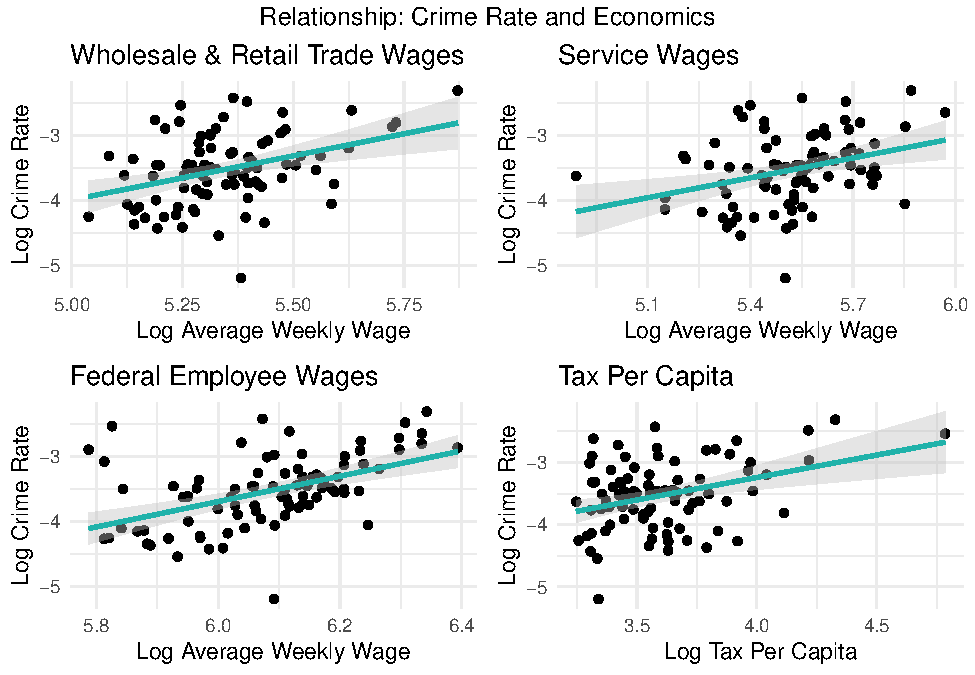
\includegraphics{lab_3_final_files/figure-latex/unnamed-chunk-34-1} 

}

\caption{Figure 11}\label{fig:unnamed-chunk-34}
\end{figure}

\hypertarget{discussion-1}{%
\paragraph{Discussion}\label{discussion-1}}

The first iteration of this model included all crime justice variable as
well as all key economic variables. In this specification, none of the
economic policy variables had statistically significant relationships to
crime. The coefficient estimates for economic context variables
(\texttt{taxpc} and \texttt{wfed}) were statistically significant and
positive. This indicates that crime rate is larger in counties with more
tax revenue and higher cost of living, controlling for the other
variables in the model. These variables could have captured part of the
crime rate variation that should be captured by demographic variables
such as \texttt{density}. We expected the estimated coefficients for
these variables to fluctuate as we add more demographic variables.

After adding economic policy and context to the model, the estimated
impact of log(\texttt{prbarr}) on log(\texttt{crmrte}) reduces only
slightly versus model set \#1 (from \textasciitilde{}0.7 to
\textasciitilde{}0.6). We conducted an F-test to determine if the
economic policy variables were jointly statistically significant at
explaining variation on crime rate. In this test, the null hypothesis
was that economic policies, proxied by average wages at lower paying
industries and at local administrations, do not have explanatory power
over crime rate. The p-value of this test was well over our alpha of .05
and thus we could not reject the hypothesis.

The exclusion of economic policy variables from our models is also
advisable according to BIC, which is smaller for the most parsimonious
model shown in column 2, our preferred specification in this set.
However, we decided to keep one proxy for wage policy - Wholesale \&
Retail Trade sector wages - because these are the closest to the minimum
wage and most likely to be affected by minimum wage policy. Keeping this
variable gives it a chance to be tested with other covariates, such as
density and percentage of minority, in our later model specifications.

\begin{Shaded}
\begin{Highlighting}[]
\NormalTok{mod2_}\DecValTok{1}\NormalTok{ <-}\StringTok{ }\KeywordTok{lm}\NormalTok{(}\KeywordTok{log}\NormalTok{(crmrte) }\OperatorTok{~}\StringTok{ }\KeywordTok{log}\NormalTok{(prbarr) }\OperatorTok{+}\StringTok{ }\KeywordTok{log}\NormalTok{(prbconv) }\OperatorTok{+}\StringTok{ }\KeywordTok{log}\NormalTok{(wtrd) }\OperatorTok{+}\StringTok{ }\KeywordTok{log}\NormalTok{(wser) }\OperatorTok{+}\StringTok{ }\KeywordTok{log}\NormalTok{(wloc) }\OperatorTok{+}\StringTok{ }\KeywordTok{log}\NormalTok{(wsta) }\OperatorTok{+}\StringTok{ }\KeywordTok{log}\NormalTok{(wfed) }\OperatorTok{+}\StringTok{ }\KeywordTok{log}\NormalTok{(taxpc), }\DataTypeTok{data =}\NormalTok{ data2)}
\CommentTok{# fit models}
\CommentTok{#mod2_2 <- lm(log(crmrte) ~ log(prbarr) + log(prbconv) + log(wfed) + log(taxpc), data = data2)  # no economic policy variables}
\CommentTok{#mod2_3 <- lm(log(crmrte) ~ log(prbarr)*log(wfed) + log(prbconv)*log(wfed) + log(wser)*log(wfed) + log(wsta)*log(wfed) + log(taxpc), data = data2)  # taxpc interactions}
\CommentTok{#mod2_4 <- lm(log(crmrte) ~ log(prbarr)*log(taxpc) + log(prbconv)*log(taxpc) + log(wser)*log(taxpc) + log(wsta)*log(taxpc) + wfed, data = data2)  # wfed interactions}
\NormalTok{mod2 <-}\StringTok{ }\KeywordTok{lm}\NormalTok{(}\KeywordTok{log}\NormalTok{(crmrte) }\OperatorTok{~}\StringTok{ }\KeywordTok{log}\NormalTok{(prbarr) }\OperatorTok{+}\StringTok{ }\KeywordTok{log}\NormalTok{(prbconv) }\OperatorTok{+}\StringTok{ }\KeywordTok{log}\NormalTok{(wtrd)  }\OperatorTok{+}\StringTok{ }\KeywordTok{log}\NormalTok{(wfed) }\OperatorTok{+}\StringTok{ }\KeywordTok{log}\NormalTok{(taxpc), }\DataTypeTok{data =}\NormalTok{ data2)   }\CommentTok{# some economic policy variables, no interactions}

\CommentTok{# generate robust standard errors}
\NormalTok{se_mod2_}\DecValTok{1}\NormalTok{ <-}\StringTok{ }\KeywordTok{sqrt}\NormalTok{(}\KeywordTok{diag}\NormalTok{(}\KeywordTok{vcovHC}\NormalTok{(mod2_}\DecValTok{1}\NormalTok{)))}
\NormalTok{se_mod2 <-}\StringTok{ }\KeywordTok{sqrt}\NormalTok{(}\KeywordTok{diag}\NormalTok{(}\KeywordTok{vcovHC}\NormalTok{(mod2)))}

\CommentTok{# produce regression table}
\KeywordTok{stargazer}\NormalTok{(}
\NormalTok{    mod2_}\DecValTok{1}
\NormalTok{  , mod2}
\NormalTok{  , }\DataTypeTok{type =} \StringTok{"text"}
\NormalTok{  , }\DataTypeTok{se =} \KeywordTok{list}\NormalTok{(se_mod2_}\DecValTok{1}\NormalTok{, se_mod2)}
\NormalTok{  , }\DataTypeTok{add.lines=}\KeywordTok{list}\NormalTok{(}\KeywordTok{c}\NormalTok{(}\StringTok{"BIC"}\NormalTok{, }\KeywordTok{round}\NormalTok{(}\KeywordTok{BIC}\NormalTok{(mod2_}\DecValTok{1}\NormalTok{),}\DecValTok{1}\NormalTok{), }\KeywordTok{round}\NormalTok{(}\KeywordTok{BIC}\NormalTok{(mod2))))}
\NormalTok{  , }\DataTypeTok{notes =} \StringTok{"Robust SE"}
\NormalTok{  , }\DataTypeTok{star.cutoffs =} \KeywordTok{c}\NormalTok{(}\FloatTok{0.05}\NormalTok{, }\FloatTok{0.01}\NormalTok{, }\FloatTok{0.001}\NormalTok{)}
\NormalTok{  )}
\end{Highlighting}
\end{Shaded}

\begin{verbatim}
## 
## =================================================================
##                                  Dependent variable:             
##                     ---------------------------------------------
##                                      log(crmrte)                 
##                              (1)                    (2)          
## -----------------------------------------------------------------
## log(prbarr)               -0.615***              -0.567***       
##                            (0.130)                (0.119)        
##                                                                  
## log(prbconv)              -0.427***              -0.402***       
##                            (0.123)                (0.121)        
##                                                                  
## log(wtrd)                   0.007                  0.074         
##                            (0.420)                (0.417)        
##                                                                  
## log(wser)                   -0.512                               
##                            (0.315)                               
##                                                                  
## log(wloc)                   0.640                                
##                            (0.699)                               
##                                                                  
## log(wsta)                   -0.266                               
##                            (0.313)                               
##                                                                  
## log(wfed)                  1.769**                1.559**        
##                            (0.573)                (0.539)        
##                                                                  
## log(taxpc)                  0.404                  0.374         
##                            (0.207)                (0.202)        
##                                                                  
## Constant                  -16.205***             -15.810***      
##                            (3.414)                (2.360)        
##                                                                  
## -----------------------------------------------------------------
## BIC                         102.7                    93          
## Observations                  89                     89          
## R2                          0.614                  0.597         
## Adjusted R2                 0.575                  0.573         
## Residual Std. Error    0.353 (df = 80)        0.354 (df = 83)    
## F Statistic         15.875*** (df = 8; 80) 24.614*** (df = 5; 83)
## =================================================================
## Note:                               *p<0.05; **p<0.01; ***p<0.001
##                                                         Robust SE
\end{verbatim}

\begin{Shaded}
\begin{Highlighting}[]
\CommentTok{# F-test: joint significance of economic policy variables}
\KeywordTok{print}\NormalTok{(}\StringTok{"F-test results for joint significance of economic policies"}\NormalTok{) }
\end{Highlighting}
\end{Shaded}

\begin{verbatim}
## [1] "F-test results for joint significance of economic policies"
\end{verbatim}

\begin{Shaded}
\begin{Highlighting}[]
\KeywordTok{linearHypothesis}\NormalTok{(mod2_}\DecValTok{1}\NormalTok{, }\KeywordTok{c}\NormalTok{(}\StringTok{"log(wser)=0"}\NormalTok{, }\StringTok{"log(wsta)=0"}\NormalTok{, }\StringTok{"log(wtrd)=0"}\NormalTok{, }\StringTok{"log(wloc)=0"}\NormalTok{), }\DataTypeTok{vcov=}\NormalTok{vcovHC)}
\end{Highlighting}
\end{Shaded}

\begin{verbatim}
## Linear hypothesis test
## 
## Hypothesis:
## log(wser) = 0
## log(wsta) = 0
## log(wtrd) = 0
## log(wloc) = 0
## 
## Model 1: restricted model
## Model 2: log(crmrte) ~ log(prbarr) + log(prbconv) + log(wtrd) + log(wser) + 
##     log(wloc) + log(wsta) + log(wfed) + log(taxpc)
## 
## Note: Coefficient covariance matrix supplied.
## 
##   Res.Df Df      F Pr(>F)
## 1     84                 
## 2     80  4 0.7892 0.5356
\end{verbatim}

\hypertarget{conclusion-1}{%
\subparagraph{Conclusion}\label{conclusion-1}}

We failed to reject the hypothesis that economic policy variables have
no impact on crime rate. Politicians might not be able to use economic
policy variables to impact crime rate, at least as captured by the
available dataset.

The results from this model set reinforces our previous section's
findings: Politicians could leverage criminal justice policies to curb
crime rate. In fact, this second model suggests that, ceteris paribus, a
10\% increase in the arrest to crime ratio would lead to a
\textasciitilde{}6\% decrease in crime rate, while a 10\% increase in
the convictions to arrests ratio would lead to a \textasciitilde{}4\%
decrease in crime rate. These estimated effects are statistically
significant and have important practical meaning.

\hypertarget{model-set-3}{%
\subsubsection{Model set \#3}\label{model-set-3}}

For our third model, we added demographic control variables to evaluate
the robustness of the relationship between crime policy, economic
policy, and crime rate when controlling for key demographic contexts in
addition to the economic context variables. We retained the one wage
variable we thought was the best proxy for minimum wage (\texttt{wtrd})
so that we can confirm that the lack of relationship was not due to
omitted demographic variables biasing our estimates. We limited wage
variables to one to avoid overfitting.

We used the following independent variables to predict crime:

\emph{Crime policy}

\begin{enumerate}
\def\labelenumi{(\arabic{enumi})}
\item
  log(\texttt{prbarr})
\item
  log(\texttt{prbconv})
\end{enumerate}

\emph{Economic policy}

\begin{enumerate}
\def\labelenumi{(\arabic{enumi})}
\setcounter{enumi}{2}
\tightlist
\item
  log(\texttt{wtrd})
\end{enumerate}

\emph{Economic context}

\begin{enumerate}
\def\labelenumi{(\arabic{enumi})}
\setcounter{enumi}{3}
\item
  log(\texttt{wfed})
\item
  log(\texttt{taxpc})
\end{enumerate}

\emph{Demographic}

\begin{enumerate}
\def\labelenumi{(\arabic{enumi})}
\setcounter{enumi}{5}
\item
  \texttt{density}
\item
  \texttt{pctymle}
\item
  \texttt{pctmin80}
\end{enumerate}

\hypertarget{data-transformations-2}{%
\paragraph{Data Transformations}\label{data-transformations-2}}

Many counties had similar demographics (\texttt{density}, \texttt{mix},
\texttt{pctymle}). This could be due to the fact that North Carolina is
a small state that may have limited demographic variation. Logarithmic
transformation is a convenient means of transforming a highly skewed
variable into a more normalized dataset. Still, plotting the log of
demographic versus the log of crime rate didn't seem to improve our fit
and we decided not to log-transform these variables.

Taking the log of \texttt{density} or \texttt{pctymle} did not improve
either of their fits to crime rate. The percent minority in 1980 did not
have a strong relationship with crime rate. Counties appear to have a
wide range of this variable and there is only a slight positive
correlation with crime rate. We noticed a slight concave form on the
scatterplot so we will try a quadratic transformation of the variable in
the model specifications below. These patterns are shown in Figure 12.

\begin{Shaded}
\begin{Highlighting}[]
\NormalTok{den1 <-}\StringTok{ }\KeywordTok{ggplot}\NormalTok{(}\DataTypeTok{data =}\NormalTok{ data2, }\KeywordTok{aes}\NormalTok{(}\DataTypeTok{x =}\NormalTok{ density, }\KeywordTok{log}\NormalTok{(crmrte))) }\OperatorTok{+}
\StringTok{  }\KeywordTok{geom_point}\NormalTok{() }\OperatorTok{+}
\StringTok{  }\KeywordTok{theme_minimal}\NormalTok{() }\OperatorTok{+}
\StringTok{  }\KeywordTok{ggtitle}\NormalTok{(}\StringTok{"Density"}\NormalTok{) }\OperatorTok{+}\StringTok{ }
\StringTok{  }\KeywordTok{ylab}\NormalTok{(}\StringTok{"Log Crime Rate"}\NormalTok{) }\OperatorTok{+}\StringTok{ }\KeywordTok{xlab}\NormalTok{(}\StringTok{"People per Sq. Mile"}\NormalTok{) }\OperatorTok{+}
\StringTok{  }\KeywordTok{geom_smooth}\NormalTok{(}\DataTypeTok{method=}\StringTok{'lm'}\NormalTok{, }\DataTypeTok{formula=}\NormalTok{ y}\OperatorTok{~}\NormalTok{x, }\DataTypeTok{color =} \KeywordTok{wes_palette}\NormalTok{(}\StringTok{"BottleRocket2"}\NormalTok{, }\DataTypeTok{n =} \DecValTok{1}\NormalTok{), }\DataTypeTok{fill =} \StringTok{"grey"}\NormalTok{)}

\NormalTok{den2 <-}\StringTok{ }\KeywordTok{ggplot}\NormalTok{(}\DataTypeTok{data =}\NormalTok{ data2, }\KeywordTok{aes}\NormalTok{(}\DataTypeTok{x =} \KeywordTok{log}\NormalTok{(density), }\KeywordTok{log}\NormalTok{(crmrte))) }\OperatorTok{+}
\StringTok{  }\KeywordTok{geom_point}\NormalTok{() }\OperatorTok{+}
\StringTok{  }\KeywordTok{theme_minimal}\NormalTok{() }\OperatorTok{+}
\StringTok{  }\KeywordTok{ggtitle}\NormalTok{(}\StringTok{"Log Density"}\NormalTok{) }\OperatorTok{+}\StringTok{ }
\StringTok{  }\KeywordTok{ylab}\NormalTok{(}\StringTok{"Log Crime Rate"}\NormalTok{) }\OperatorTok{+}\StringTok{ }\KeywordTok{xlab}\NormalTok{(}\StringTok{"Log People per Sq. Mile"}\NormalTok{) }\OperatorTok{+}
\StringTok{  }\KeywordTok{geom_smooth}\NormalTok{(}\DataTypeTok{method=}\StringTok{'lm'}\NormalTok{, }\DataTypeTok{formula=}\NormalTok{ y}\OperatorTok{~}\NormalTok{x, }\DataTypeTok{color =} \KeywordTok{wes_palette}\NormalTok{(}\StringTok{"BottleRocket2"}\NormalTok{, }\DataTypeTok{n =} \DecValTok{1}\NormalTok{), }\DataTypeTok{fill =} \StringTok{"grey"}\NormalTok{)}

\NormalTok{ymle1 <-}\StringTok{ }\KeywordTok{ggplot}\NormalTok{(}\DataTypeTok{data =}\NormalTok{ data2, }\KeywordTok{aes}\NormalTok{(}\DataTypeTok{x =}\NormalTok{ pctymle, }\KeywordTok{log}\NormalTok{(crmrte))) }\OperatorTok{+}
\StringTok{  }\KeywordTok{geom_point}\NormalTok{() }\OperatorTok{+}
\StringTok{  }\KeywordTok{theme_minimal}\NormalTok{() }\OperatorTok{+}
\StringTok{  }\KeywordTok{ggtitle}\NormalTok{(}\StringTok{"Percent Young Male"}\NormalTok{) }\OperatorTok{+}\StringTok{ }
\StringTok{  }\KeywordTok{ylab}\NormalTok{(}\StringTok{"Log Crime Rate"}\NormalTok{) }\OperatorTok{+}\StringTok{ }\KeywordTok{xlab}\NormalTok{(}\StringTok{"% Young Male"}\NormalTok{) }\OperatorTok{+}
\StringTok{  }\KeywordTok{geom_smooth}\NormalTok{(}\DataTypeTok{method=}\StringTok{'lm'}\NormalTok{, }\DataTypeTok{formula=}\NormalTok{ y}\OperatorTok{~}\NormalTok{x, }\DataTypeTok{color =} \KeywordTok{wes_palette}\NormalTok{(}\StringTok{"BottleRocket2"}\NormalTok{, }\DataTypeTok{n =} \DecValTok{1}\NormalTok{), }\DataTypeTok{fill =} \StringTok{"grey"}\NormalTok{)}

\NormalTok{ymle2 <-}\StringTok{ }\KeywordTok{ggplot}\NormalTok{(}\DataTypeTok{data =}\NormalTok{ data2, }\KeywordTok{aes}\NormalTok{(}\DataTypeTok{x =} \KeywordTok{log}\NormalTok{(pctymle), }\KeywordTok{log}\NormalTok{(crmrte))) }\OperatorTok{+}
\StringTok{  }\KeywordTok{geom_point}\NormalTok{() }\OperatorTok{+}
\StringTok{  }\KeywordTok{theme_minimal}\NormalTok{() }\OperatorTok{+}
\StringTok{  }\KeywordTok{ggtitle}\NormalTok{(}\StringTok{"Log Percent Young Male"}\NormalTok{) }\OperatorTok{+}\StringTok{ }
\StringTok{  }\KeywordTok{ylab}\NormalTok{(}\StringTok{"Log Crime Rate"}\NormalTok{) }\OperatorTok{+}\StringTok{ }\KeywordTok{xlab}\NormalTok{(}\StringTok{"Log % Young Male"}\NormalTok{) }\OperatorTok{+}
\StringTok{  }\KeywordTok{geom_smooth}\NormalTok{(}\DataTypeTok{method=}\StringTok{'lm'}\NormalTok{, }\DataTypeTok{formula=}\NormalTok{ y}\OperatorTok{~}\NormalTok{x, }\DataTypeTok{color =} \KeywordTok{wes_palette}\NormalTok{(}\StringTok{"BottleRocket2"}\NormalTok{, }\DataTypeTok{n =} \DecValTok{1}\NormalTok{), }\DataTypeTok{fill =} \StringTok{"grey"}\NormalTok{)}

\NormalTok{min1 <-}\StringTok{ }\KeywordTok{ggplot}\NormalTok{(}\DataTypeTok{data =}\NormalTok{ data2, }\KeywordTok{aes}\NormalTok{(}\DataTypeTok{x =}\NormalTok{ pctmin80, }\KeywordTok{log}\NormalTok{(crmrte))) }\OperatorTok{+}
\StringTok{  }\KeywordTok{geom_point}\NormalTok{() }\OperatorTok{+}
\StringTok{  }\KeywordTok{theme_minimal}\NormalTok{() }\OperatorTok{+}
\StringTok{  }\KeywordTok{ggtitle}\NormalTok{(}\StringTok{"Percent Minority"}\NormalTok{) }\OperatorTok{+}\StringTok{ }
\StringTok{  }\KeywordTok{ylab}\NormalTok{(}\StringTok{"Log Crime Rate"}\NormalTok{) }\OperatorTok{+}\StringTok{ }\KeywordTok{xlab}\NormalTok{(}\StringTok{"% Minority"}\NormalTok{) }\OperatorTok{+}
\StringTok{  }\KeywordTok{geom_smooth}\NormalTok{(}\DataTypeTok{method=}\StringTok{'lm'}\NormalTok{, }\DataTypeTok{formula=}\NormalTok{ y}\OperatorTok{~}\NormalTok{x, }\DataTypeTok{color =} \KeywordTok{wes_palette}\NormalTok{(}\StringTok{"BottleRocket2"}\NormalTok{, }\DataTypeTok{n =} \DecValTok{1}\NormalTok{), }\DataTypeTok{fill =} \StringTok{"grey"}\NormalTok{)}

\NormalTok{min2 <-}\StringTok{ }\KeywordTok{ggplot}\NormalTok{(}\DataTypeTok{data =}\NormalTok{ data2, }\KeywordTok{aes}\NormalTok{(}\DataTypeTok{x =}\NormalTok{ pctmin80}\OperatorTok{*}\NormalTok{pctmin80, }\KeywordTok{log}\NormalTok{(crmrte))) }\OperatorTok{+}
\StringTok{  }\KeywordTok{geom_point}\NormalTok{() }\OperatorTok{+}
\StringTok{  }\KeywordTok{theme_minimal}\NormalTok{() }\OperatorTok{+}
\StringTok{  }\KeywordTok{ggtitle}\NormalTok{(}\StringTok{"Percent Minority^2"}\NormalTok{) }\OperatorTok{+}\StringTok{ }
\StringTok{  }\KeywordTok{ylab}\NormalTok{(}\StringTok{"Log Crime Rate"}\NormalTok{) }\OperatorTok{+}\StringTok{ }\KeywordTok{xlab}\NormalTok{(}\StringTok{"% Minority^2"}\NormalTok{) }\OperatorTok{+}
\StringTok{  }\KeywordTok{geom_smooth}\NormalTok{(}\DataTypeTok{method=}\StringTok{'lm'}\NormalTok{, }\DataTypeTok{formula=}\NormalTok{ y }\OperatorTok{~}\NormalTok{x }\OperatorTok{+}\StringTok{ }\KeywordTok{I}\NormalTok{(x}\OperatorTok{^}\DecValTok{2}\NormalTok{), }\DataTypeTok{color =} \KeywordTok{wes_palette}\NormalTok{(}\StringTok{"BottleRocket2"}\NormalTok{, }\DataTypeTok{n =} \DecValTok{1}\NormalTok{), }\DataTypeTok{fill =} \StringTok{"grey"}\NormalTok{)}

\KeywordTok{grid.arrange}\NormalTok{(den1, den2, ymle1, ymle2, min1, min2, }\DataTypeTok{ncol =} \DecValTok{2}\NormalTok{, }\DataTypeTok{nrow =} \DecValTok{3}\NormalTok{, }\DataTypeTok{top =} \StringTok{"Relationship: Crime Rate and Demographics"}\NormalTok{)}
\end{Highlighting}
\end{Shaded}

\begin{figure}

{\centering 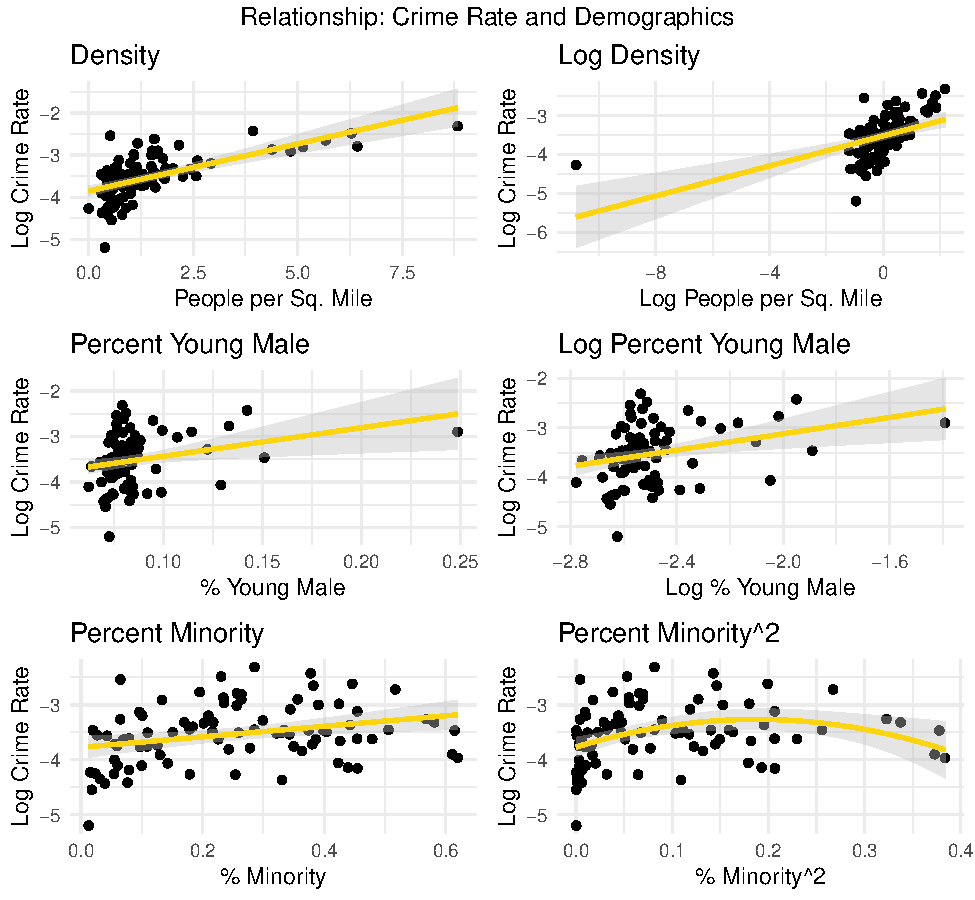
\includegraphics{lab_3_final_files/figure-latex/unnamed-chunk-37-1} 

}

\caption{Figure 12}\label{fig:unnamed-chunk-37}
\end{figure}

\hypertarget{discussion-2}{%
\paragraph{Discussion}\label{discussion-2}}

The first iteration (column 1) of this model set includes all the
variables listed above. Including all factors related to the
demographics improves our model (lower BIC and larger adjusted R2
vs.~model set \#2).

Among all demographic variables included, only \texttt{pctymle} is not
individually significant. An F-test was conducted with results leading
us to reject the null that the demographic variables are not jointly
significant.

In the following iteration (column 2), we added a quadratic
transformation of percent minority, in an attempt to capture the
seemingly concave relationship of this variable with
log(\texttt{crmrte}) discussed above. However, the coefficient on the
quadratic transformation of percent minority was not statistically
significant and the model's BIC is slightly larger than in column 1,
leading us to give up on column 2 specification. In column 3, we dropped
\texttt{pctymle}, leading to a larger BIC vs.~column 1. This fact and
our understanding that \texttt{pctymle} is an important control in crime
rate models made us decide to keep the variable.

Given the above, our preferred equation in the model set \#3 was column
1. The above also led us to conclude that that demographic factors
should be part of of our model. Higher rates of any of these are related
to higher levels of crime.

Our economic policy proxy does not seem to be statistically significant
in explaining variation in crime rate when modeled with or without the
addition of demographic control variables. As we noted above, this could
be due to omitted variable bias and/or the fact that (even lower-income)
average wages are imperfect proxies for minimum wage.

\begin{Shaded}
\begin{Highlighting}[]
\NormalTok{data2}\OperatorTok{$}\NormalTok{pctmin802 =}\StringTok{ }\NormalTok{data2}\OperatorTok{$}\NormalTok{pctmin80}\OperatorTok{*}\NormalTok{data2}\OperatorTok{$}\NormalTok{pctmin80}

\CommentTok{# fit models}
\NormalTok{mod3_}\DecValTok{1}\NormalTok{ <-}\StringTok{ }\KeywordTok{lm}\NormalTok{(}\KeywordTok{log}\NormalTok{(crmrte) }\OperatorTok{~}\StringTok{ }\KeywordTok{log}\NormalTok{(prbarr) }\OperatorTok{+}\StringTok{ }\KeywordTok{log}\NormalTok{(prbconv) }\OperatorTok{+}\StringTok{ }\KeywordTok{log}\NormalTok{(wtrd)  }\OperatorTok{+}\StringTok{ }\KeywordTok{log}\NormalTok{(wfed) }\OperatorTok{+}\StringTok{ }\KeywordTok{log}\NormalTok{(taxpc) }\OperatorTok{+}\StringTok{ }\NormalTok{density }\OperatorTok{+}\StringTok{ }\NormalTok{pctmin80 }\OperatorTok{+}\StringTok{ }\NormalTok{pctymle, }\DataTypeTok{data =}\NormalTok{ data2)  }\CommentTok{# all vars}
\NormalTok{mod3_}\DecValTok{2}\NormalTok{ <-}\StringTok{ }\KeywordTok{lm}\NormalTok{(}\KeywordTok{log}\NormalTok{(crmrte) }\OperatorTok{~}\StringTok{ }\KeywordTok{log}\NormalTok{(prbarr) }\OperatorTok{+}\StringTok{ }\KeywordTok{log}\NormalTok{(prbconv) }\OperatorTok{+}\StringTok{ }\KeywordTok{log}\NormalTok{(wtrd) }\OperatorTok{+}\StringTok{ }\KeywordTok{log}\NormalTok{(wfed) }\OperatorTok{+}\StringTok{ }\KeywordTok{log}\NormalTok{(taxpc) }\OperatorTok{+}\StringTok{ }\NormalTok{density }\OperatorTok{+}\StringTok{ }\NormalTok{pctmin80 }\OperatorTok{+}\StringTok{ }\NormalTok{pctmin802 }\OperatorTok{+}\StringTok{ }\NormalTok{pctymle, }\DataTypeTok{data =}\NormalTok{ data2)  }\CommentTok{# pctmin80 quadratic transform}
\NormalTok{mod3_}\DecValTok{3}\NormalTok{ <-}\StringTok{ }\KeywordTok{lm}\NormalTok{(}\KeywordTok{log}\NormalTok{(crmrte) }\OperatorTok{~}\StringTok{ }\KeywordTok{log}\NormalTok{(prbarr) }\OperatorTok{+}\StringTok{ }\KeywordTok{log}\NormalTok{(prbconv) }\OperatorTok{+}\StringTok{ }\KeywordTok{log}\NormalTok{(wtrd) }\OperatorTok{+}\StringTok{ }\KeywordTok{log}\NormalTok{(wfed) }\OperatorTok{+}\StringTok{ }\KeywordTok{log}\NormalTok{(taxpc) }\OperatorTok{+}\StringTok{ }\NormalTok{density }\OperatorTok{+}\StringTok{ }\NormalTok{pctmin80 , }\DataTypeTok{data =}\NormalTok{ data2)  }\CommentTok{# no pctymle}
\CommentTok{#mod3_4 <- lm(log(crmrte) ~ log(prbarr) + log(prbconv) + log(wfed) + log(taxpc) + density + pctmin80 + pctymle, data = data2)  # no wages}

\CommentTok{# generate robust standard errors}
\NormalTok{se_mod3_}\DecValTok{1}\NormalTok{ <-}\StringTok{ }\KeywordTok{sqrt}\NormalTok{(}\KeywordTok{diag}\NormalTok{(}\KeywordTok{vcovHC}\NormalTok{(mod3_}\DecValTok{1}\NormalTok{)))}
\NormalTok{se_mod3_}\DecValTok{2}\NormalTok{ <-}\StringTok{ }\KeywordTok{sqrt}\NormalTok{(}\KeywordTok{diag}\NormalTok{(}\KeywordTok{vcovHC}\NormalTok{(mod3_}\DecValTok{2}\NormalTok{)))}
\NormalTok{se_mod3_}\DecValTok{3}\NormalTok{ <-}\StringTok{ }\KeywordTok{sqrt}\NormalTok{(}\KeywordTok{diag}\NormalTok{(}\KeywordTok{vcovHC}\NormalTok{(mod3_}\DecValTok{3}\NormalTok{)))}
\CommentTok{#se_mod3_4 <- sqrt(diag(vcovHC(mod3_4)))}

\CommentTok{# produce regression table}
\KeywordTok{stargazer}\NormalTok{(}
\NormalTok{    mod3_}\DecValTok{1}
\NormalTok{  , mod3_}\DecValTok{2}
\NormalTok{  , mod3_}\DecValTok{3}
  \CommentTok{#, mod3_4}
\NormalTok{  , }\DataTypeTok{type =} \StringTok{"text"}
\NormalTok{  , }\DataTypeTok{se =} \KeywordTok{list}\NormalTok{(se_mod3_}\DecValTok{1}\NormalTok{, se_mod3_}\DecValTok{2}\NormalTok{, se_mod3_}\DecValTok{3}\NormalTok{)}
\NormalTok{  , }\DataTypeTok{star.cutoffs =} \KeywordTok{c}\NormalTok{(}\FloatTok{0.05}\NormalTok{, }\FloatTok{0.01}\NormalTok{, }\FloatTok{0.001}\NormalTok{)}
\NormalTok{  , }\DataTypeTok{notes =} \KeywordTok{c}\NormalTok{(}\StringTok{"Robust SE"}\NormalTok{)}
\NormalTok{  , }\DataTypeTok{add.lines=}\KeywordTok{list}\NormalTok{(}\KeywordTok{c}\NormalTok{(}\StringTok{"BIC"}\NormalTok{, }\KeywordTok{round}\NormalTok{(}\KeywordTok{BIC}\NormalTok{(mod3_}\DecValTok{1}\NormalTok{),}\DecValTok{1}\NormalTok{), }\KeywordTok{round}\NormalTok{(}\KeywordTok{BIC}\NormalTok{(mod3_}\DecValTok{2}\NormalTok{),}\DecValTok{1}\NormalTok{) , }\KeywordTok{round}\NormalTok{(}\KeywordTok{BIC}\NormalTok{(mod3_}\DecValTok{3}\NormalTok{),}\DecValTok{1}\NormalTok{) }
                     \CommentTok{#, round(BIC(mod3_4),1)}
\NormalTok{                     )}
\NormalTok{                   )}
\NormalTok{  )}
\end{Highlighting}
\end{Shaded}

\begin{verbatim}
## 
## ========================================================================================
##                                             Dependent variable:                         
##                     --------------------------------------------------------------------
##                                                 log(crmrte)                             
##                              (1)                    (2)                    (3)          
## ----------------------------------------------------------------------------------------
## log(prbarr)               -0.504***              -0.478***              -0.559***       
##                            (0.110)                (0.126)                (0.089)        
##                                                                                         
## log(prbconv)               -0.329**               -0.326**              -0.363***       
##                            (0.100)                (0.101)                (0.094)        
##                                                                                         
## log(wtrd)                   0.075                  0.032                  -0.008        
##                            (0.373)                (0.376)                (0.341)        
##                                                                                         
## log(wfed)                   1.072*                 1.096*                 1.002*        
##                            (0.427)                (0.431)                (0.444)        
##                                                                                         
## log(taxpc)                  0.289                  0.269                  0.230         
##                            (0.317)                (0.362)                (0.322)        
##                                                                                         
## density                     0.079                  0.077                  0.089*        
##                            (0.043)                (0.043)                (0.045)        
##                                                                                         
## pctmin80                   1.127***                1.841                 1.153***       
##                            (0.214)                (0.978)                (0.210)        
##                                                                                         
## pctmin802                                          -1.295                               
##                                                   (1.551)                               
##                                                                                         
## pctymle                     3.087                  3.008                                
##                            (3.491)                (3.279)                               
##                                                                                         
## Constant                  -13.064***             -12.921***             -11.835***      
##                            (2.256)                (2.283)                (2.650)        
##                                                                                         
## ----------------------------------------------------------------------------------------
## BIC                          62.6                   65.7                   63.1         
## Observations                  89                     89                     89          
## R2                          0.754                  0.758                  0.740         
## Adjusted R2                 0.729                  0.730                  0.717         
## Residual Std. Error    0.282 (df = 80)        0.282 (df = 79)        0.288 (df = 81)    
## F Statistic         30.642*** (df = 8; 80) 27.426*** (df = 9; 79) 32.863*** (df = 7; 81)
## ========================================================================================
## Note:                                                      *p<0.05; **p<0.01; ***p<0.001
##                                                                                Robust SE
\end{verbatim}

\begin{Shaded}
\begin{Highlighting}[]
\NormalTok{mod3 <-}\StringTok{ }\NormalTok{mod3_}\DecValTok{1}
\NormalTok{se_mod3 <-}\StringTok{ }\NormalTok{se_mod3_}\DecValTok{1}
\end{Highlighting}
\end{Shaded}

\begin{Shaded}
\begin{Highlighting}[]
\CommentTok{# F-test: joint significance of demographic variables}
\KeywordTok{print}\NormalTok{(}\StringTok{"F-test results for joint significance of demographic variables"}\NormalTok{) }
\end{Highlighting}
\end{Shaded}

\begin{verbatim}
## [1] "F-test results for joint significance of demographic variables"
\end{verbatim}

\begin{Shaded}
\begin{Highlighting}[]
\KeywordTok{linearHypothesis}\NormalTok{(mod3_}\DecValTok{1}\NormalTok{, }\KeywordTok{c}\NormalTok{(}\StringTok{"density=0"}\NormalTok{, }\StringTok{"pctmin80=0"}\NormalTok{, }\StringTok{"pctymle=0"}\NormalTok{), }\DataTypeTok{vcov=}\NormalTok{vcovHC)}
\end{Highlighting}
\end{Shaded}

\begin{verbatim}
## Linear hypothesis test
## 
## Hypothesis:
## density = 0
## pctmin80 = 0
## pctymle = 0
## 
## Model 1: restricted model
## Model 2: log(crmrte) ~ log(prbarr) + log(prbconv) + log(wtrd) + log(wfed) + 
##     log(taxpc) + density + pctmin80 + pctymle
## 
## Note: Coefficient covariance matrix supplied.
## 
##   Res.Df Df      F    Pr(>F)    
## 1     83                        
## 2     80  3 9.6385 1.673e-05 ***
## ---
## Signif. codes:  0 '***' 0.001 '**' 0.01 '*' 0.05 '.' 0.1 ' ' 1
\end{verbatim}

\hypertarget{outliers}{%
\subparagraph{Outliers}\label{outliers}}

Figure 13 shows that there are 2 observations labeled as outliers and
high leverage points (which is to be expected since they were at the
extremes of some of our predictor variables). These labels correspond to
the row numbers but we list their county numbers below for easier
comprehension.

\begin{itemize}
\tightlist
\item
  observation 6 - county 11
\item
  observation 25 - county 55
\end{itemize}

\begin{Shaded}
\begin{Highlighting}[]
\KeywordTok{ols_plot_resid_lev}\NormalTok{(mod3)}
\end{Highlighting}
\end{Shaded}

\begin{figure}

{\centering 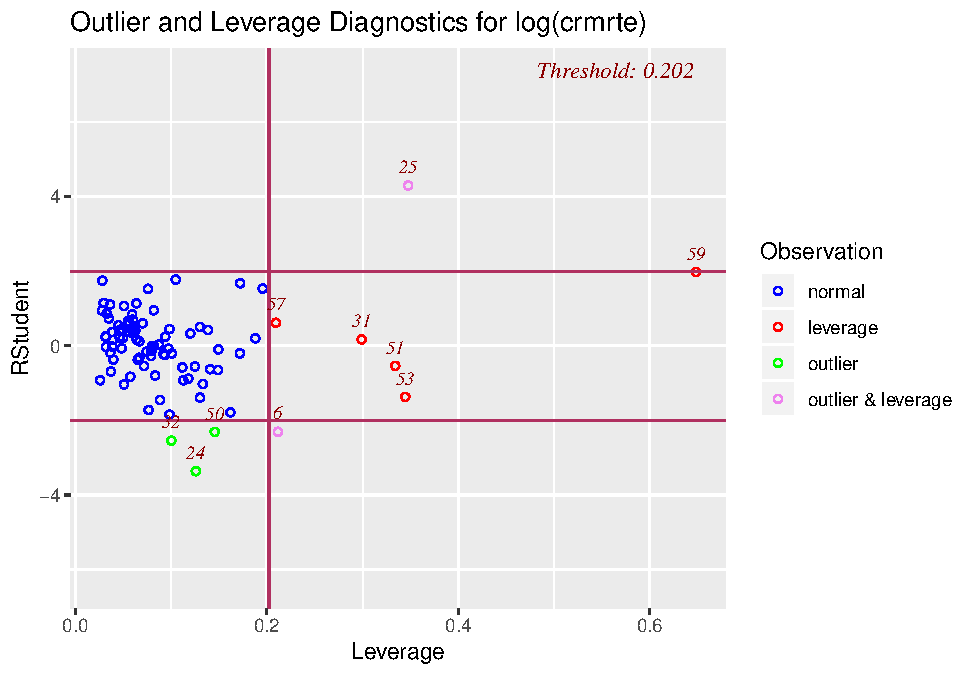
\includegraphics{lab_3_final_files/figure-latex/unnamed-chunk-40-1} 

}

\caption{Figure 13}\label{fig:unnamed-chunk-40}
\end{figure}

\emph{Do these two counties influence our model fits?} We can see that
without these observations, we now explain a bit more of the variation.
Although eliminating these have improved our fit, we do not have any
reason to suspect that they have data quality issues. Dropping any of
these do not change our conclusions around our main predictor variables.

\begin{Shaded}
\begin{Highlighting}[]
\CommentTok{# county 11}
\NormalTok{mod3_out11 <-}\StringTok{ }\KeywordTok{lm}\NormalTok{(}\KeywordTok{log}\NormalTok{(crmrte) }\OperatorTok{~}\StringTok{ }\KeywordTok{log}\NormalTok{(prbarr) }\OperatorTok{+}\StringTok{ }\KeywordTok{log}\NormalTok{(prbconv) }\OperatorTok{+}\StringTok{ }\KeywordTok{log}\NormalTok{(wtrd)  }\OperatorTok{+}\StringTok{ }\KeywordTok{log}\NormalTok{(wfed) }\OperatorTok{+}\StringTok{ }\KeywordTok{log}\NormalTok{(taxpc) }\OperatorTok{+}\StringTok{ }\NormalTok{density }\OperatorTok{+}\StringTok{ }\NormalTok{pctmin80 }\OperatorTok{+}\StringTok{ }\NormalTok{pctymle, }\DataTypeTok{data =} \KeywordTok{filter}\NormalTok{(data2, county }\OperatorTok{!=}\StringTok{ }\DecValTok{11}\NormalTok{)) }

\NormalTok{se_mod3_out11 <-}\StringTok{ }\KeywordTok{sqrt}\NormalTok{(}\KeywordTok{diag}\NormalTok{(}\KeywordTok{vcovHC}\NormalTok{(mod3_out11)))}

\CommentTok{# county 55}
\NormalTok{mod3_out55 <-}\StringTok{ }\KeywordTok{lm}\NormalTok{(}\KeywordTok{log}\NormalTok{(crmrte) }\OperatorTok{~}\StringTok{ }\KeywordTok{log}\NormalTok{(prbarr) }\OperatorTok{+}\StringTok{ }\KeywordTok{log}\NormalTok{(prbconv) }\OperatorTok{+}\StringTok{ }\KeywordTok{log}\NormalTok{(wtrd)  }\OperatorTok{+}\StringTok{ }\KeywordTok{log}\NormalTok{(wfed) }\OperatorTok{+}\StringTok{ }\KeywordTok{log}\NormalTok{(taxpc) }\OperatorTok{+}\StringTok{ }\NormalTok{density }\OperatorTok{+}\StringTok{ }\NormalTok{pctmin80 }\OperatorTok{+}\StringTok{ }\NormalTok{pctymle, }\DataTypeTok{data =} \KeywordTok{filter}\NormalTok{(data2, county }\OperatorTok{!=}\StringTok{ }\DecValTok{55}\NormalTok{)) }

\NormalTok{se_mod3_out55 <-}\StringTok{ }\KeywordTok{sqrt}\NormalTok{(}\KeywordTok{diag}\NormalTok{(}\KeywordTok{vcovHC}\NormalTok{(mod3_out55)))}

\CommentTok{# county 11 and 55}
\NormalTok{mod3_out11_}\DecValTok{55}\NormalTok{ <-}\StringTok{ }\KeywordTok{lm}\NormalTok{(}\KeywordTok{log}\NormalTok{(crmrte) }\OperatorTok{~}\StringTok{ }\KeywordTok{log}\NormalTok{(prbarr) }\OperatorTok{+}\StringTok{ }\KeywordTok{log}\NormalTok{(prbconv) }\OperatorTok{+}\StringTok{ }\KeywordTok{log}\NormalTok{(wtrd)  }\OperatorTok{+}\StringTok{ }\KeywordTok{log}\NormalTok{(wfed) }\OperatorTok{+}\StringTok{ }\KeywordTok{log}\NormalTok{(taxpc) }\OperatorTok{+}\StringTok{ }\NormalTok{density }\OperatorTok{+}\StringTok{ }\NormalTok{pctmin80 }\OperatorTok{+}\StringTok{ }\NormalTok{pctymle, }\DataTypeTok{data =} \KeywordTok{filter}\NormalTok{(data2, county }\OperatorTok{!=}\StringTok{ }\DecValTok{11} \OperatorTok{&}\StringTok{ }\NormalTok{county }\OperatorTok{!=}\StringTok{ }\DecValTok{55}\NormalTok{)) }

\NormalTok{se_mod3_out11_}\DecValTok{55}\NormalTok{ <-}\StringTok{ }\KeywordTok{sqrt}\NormalTok{(}\KeywordTok{diag}\NormalTok{(}\KeywordTok{vcovHC}\NormalTok{(mod3_out11_}\DecValTok{55}\NormalTok{)))}

\KeywordTok{stargazer}\NormalTok{(}
\NormalTok{    mod3}
\NormalTok{  , mod3_out11}
\NormalTok{  , mod3_out55}
\NormalTok{  , mod3_out11_}\DecValTok{55}
\NormalTok{  , }\DataTypeTok{type =} \StringTok{"text"}
\NormalTok{  , }\DataTypeTok{se =} \KeywordTok{list}\NormalTok{(se_mod3_out11, se_mod3_out55, se_mod3_out11_}\DecValTok{55}\NormalTok{)}
\NormalTok{  , }\DataTypeTok{star.cutoffs =} \KeywordTok{c}\NormalTok{(}\FloatTok{0.05}\NormalTok{, }\FloatTok{0.01}\NormalTok{, }\FloatTok{0.001}\NormalTok{)}
\NormalTok{  , }\DataTypeTok{column.labels =} \KeywordTok{c}\NormalTok{(}\StringTok{"With"}\NormalTok{, }\StringTok{"Omit 11"}\NormalTok{, }\StringTok{"Omit 55"}\NormalTok{, }\StringTok{"Omit 11 and 55"}\NormalTok{) }
\NormalTok{  , }\DataTypeTok{notes =} \KeywordTok{c}\NormalTok{(}\StringTok{"Robust SE"}\NormalTok{)}
\NormalTok{)}
\end{Highlighting}
\end{Shaded}

\begin{verbatim}
## 
## ===============================================================================================================
##                                                         Dependent variable:                                    
##                     -------------------------------------------------------------------------------------------
##                                                             log(crmrte)                                        
##                              With                 Omit 11                Omit 55             Omit 11 and 55    
##                              (1)                    (2)                    (3)                    (4)          
## ---------------------------------------------------------------------------------------------------------------
## log(prbarr)               -0.504***              -0.486***              -0.459***              -0.446***       
##                            (0.107)                (0.107)                (0.106)                (0.079)        
##                                                                                                                
## log(prbconv)              -0.329***              -0.385***              -0.300***              -0.349***       
##                            (0.100)                (0.089)                (0.089)                (0.062)        
##                                                                                                                
## log(wtrd)                   0.075                  0.032                  0.021                  -0.014        
##                            (0.372)                (0.344)                (0.345)                (0.251)        
##                                                                                                                
## log(wfed)                  1.072**                1.122**                1.217**                1.253***       
##                            (0.409)                (0.393)                (0.385)                (0.279)        
##                                                                                                                
## log(taxpc)                  0.289                  0.276                  -0.005                 -0.002        
##                            (0.302)                (0.179)                (0.180)                (0.131)        
##                                                                                                                
## density                     0.079                  0.074*                0.106**                0.100***       
##                            (0.042)                (0.034)                (0.034)                (0.027)        
##                                                                                                                
## pctmin80                   1.127***               1.050***               1.231***               1.161***       
##                            (0.212)                (0.192)                (0.189)                (0.169)        
##                                                                                                                
## pctymle                     3.087                  3.147                  3.146                  3.194*        
##                            (3.131)                (3.152)                (2.859)                (1.265)        
##                                                                                                                
## Constant                  -13.064***             -13.079***             -12.601***             -12.633***      
##                            (2.257)                (2.243)                (2.229)                (1.730)        
##                                                                                                                
## ---------------------------------------------------------------------------------------------------------------
## Observations                  89                     88                     88                     87          
## R2                          0.754                  0.765                  0.793                  0.800         
## Adjusted R2                 0.729                  0.741                  0.772                  0.780         
## Residual Std. Error    0.282 (df = 80)        0.275 (df = 79)        0.255 (df = 79)        0.250 (df = 78)    
## F Statistic         30.642*** (df = 8; 80) 32.147*** (df = 8; 79) 37.737*** (df = 8; 79) 39.104*** (df = 8; 78)
## ===============================================================================================================
## Note:                                                                             *p<0.05; **p<0.01; ***p<0.001
##                                                                                                       Robust SE
\end{verbatim}

\hypertarget{conclusion-2}{%
\subparagraph{Conclusion}\label{conclusion-2}}

The most important takeaways from model set \#3 are (1) the estimated
effect of criminal justice policies on crime rate is robust to the
inclusion of demographic controls, and (2) even controlling for
demographics, the coefficient on our proxy for economic policy
(log(\texttt{wtrd})) remains statistically not significant. Besides, we
rejected the null hypothesis that demographic covariates are not related
to crime rate.

To summarize, this third model set featuring criminal justice, economic
policies, economic context as well demographic variables suggests that,
ceteris paribus, a 10\% increase in the arrests to crimes ratio would
lead to a \textasciitilde{}5\% decrease in crime rate, while a 10\%
increase in convictions to arrests ratio would lead to a
\textasciitilde{}4\% decrease in crime rate. These estimated effects are
statistically significant and have important practical meaning.
Politicians should adjust criminal justice system policies depending on
demographic variables.

\hypertarget{model-set-4}{%
\subsubsection{Model set \#4}\label{model-set-4}}

For our fourth model, we aimed to evaluate the robustness of the
relationship between crime policy and crime when controlling for
economic, demographic, and geographic context variables. In addition, we
will also reassessed the impact of economic policy on crime rate.

We used the following independent variables to predict crime:

\emph{Crime policy}

\begin{enumerate}
\def\labelenumi{(\arabic{enumi})}
\item
  log(\texttt{prbarr})
\item
  log(\texttt{prbconv})
\end{enumerate}

\emph{Economic policy}

\begin{enumerate}
\def\labelenumi{(\arabic{enumi})}
\setcounter{enumi}{2}
\tightlist
\item
  log(\texttt{wtrd})
\end{enumerate}

\emph{Economic context}

\begin{enumerate}
\def\labelenumi{(\arabic{enumi})}
\setcounter{enumi}{3}
\item
  log(\texttt{wfed})
\item
  log(\texttt{taxpc})
\end{enumerate}

\emph{Demographic}

\begin{enumerate}
\def\labelenumi{(\arabic{enumi})}
\setcounter{enumi}{5}
\item
  \texttt{density}
\item
  \texttt{pctymle}
\item
  \texttt{pctmin80}
\end{enumerate}

\emph{Geographic}

\begin{enumerate}
\def\labelenumi{(\arabic{enumi})}
\setcounter{enumi}{8}
\item
  \texttt{west}
\item
  \texttt{central}
\item
  \texttt{urban}
\end{enumerate}

\hypertarget{discussion-3}{%
\paragraph{Discussion}\label{discussion-3}}

Figure 14 shows that different geographies show the same pattern when it
comes to urban versus rural: rural counties have a lower crime rate
compared to urban ones (as expected). However, \texttt{urban} and
\texttt{density} are highly correlated as seen early, so adding
\texttt{urban} to the model may not improve fits. We can also see that
central and eastern counties are more similar in terms of crime rate
versus western counties, which have lower crime overall. Thus, we don't
expect the covariate for \texttt{central} to be significant.

\begin{Shaded}
\begin{Highlighting}[]
\CommentTok{# plot barplots}
\KeywordTok{ggplot}\NormalTok{(geo_long, }\KeywordTok{aes}\NormalTok{(}\DataTypeTok{x =}\NormalTok{ location, }\DataTypeTok{y =}\NormalTok{ crmrte, }\DataTypeTok{fill =}\NormalTok{ type)) }\OperatorTok{+}
\StringTok{  }\KeywordTok{geom_bar}\NormalTok{(}\DataTypeTok{position=}\StringTok{"dodge"}\NormalTok{, }\DataTypeTok{stat=}\StringTok{"summary"}\NormalTok{) }\OperatorTok{+}
\StringTok{  }\KeywordTok{scale_fill_manual}\NormalTok{(}\DataTypeTok{values =} \KeywordTok{wes_palette}\NormalTok{(}\StringTok{"GrandBudapest1"}\NormalTok{, }\DataTypeTok{n =} \DecValTok{3}\NormalTok{)) }\OperatorTok{+}\StringTok{ }
\StringTok{  }\KeywordTok{theme_minimal}\NormalTok{() }\OperatorTok{+}
\StringTok{  }\KeywordTok{ggtitle}\NormalTok{(}\StringTok{"Barplot of Contextual Variables: Geography"}\NormalTok{) }\OperatorTok{+}
\StringTok{  }\KeywordTok{xlab}\NormalTok{(}\StringTok{""}\NormalTok{) }\OperatorTok{+}
\StringTok{  }\KeywordTok{ylab}\NormalTok{(}\StringTok{"Average Crime Rate"}\NormalTok{)}
\end{Highlighting}
\end{Shaded}

\begin{verbatim}
## No summary function supplied, defaulting to `mean_se()
\end{verbatim}

\begin{figure}

{\centering 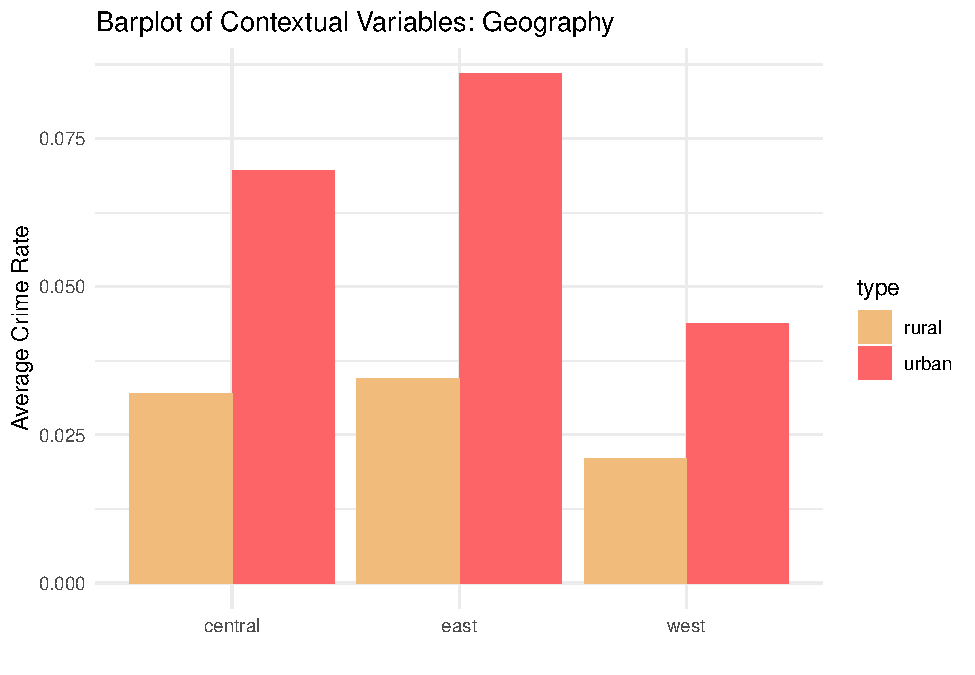
\includegraphics{lab_3_final_files/figure-latex/unnamed-chunk-42-1} 

}

\caption{Figure 14}\label{fig:unnamed-chunk-42}
\end{figure}

\emph{Statistics Interpretation}

\begin{Shaded}
\begin{Highlighting}[]
\NormalTok{mod4_}\DecValTok{1}\NormalTok{ <-}\StringTok{ }\KeywordTok{lm}\NormalTok{(}\KeywordTok{log}\NormalTok{(crmrte) }\OperatorTok{~}\StringTok{ }\KeywordTok{log}\NormalTok{(prbarr) }\OperatorTok{+}\StringTok{ }\KeywordTok{log}\NormalTok{(prbconv) }\OperatorTok{+}\StringTok{ }\KeywordTok{log}\NormalTok{(wtrd)  }\OperatorTok{+}\StringTok{ }\KeywordTok{log}\NormalTok{(wfed) }\OperatorTok{+}\StringTok{ }\KeywordTok{log}\NormalTok{(taxpc) }\OperatorTok{+}\StringTok{ }\NormalTok{density }\OperatorTok{+}\StringTok{ }\NormalTok{pctmin80 }\OperatorTok{+}\StringTok{ }\NormalTok{pctymle }\OperatorTok{+}\StringTok{ }\NormalTok{west }\OperatorTok{+}\StringTok{ }\NormalTok{central }\OperatorTok{+}\StringTok{ }\NormalTok{urban, }\DataTypeTok{data =}\NormalTok{ data2)}
\NormalTok{mod4_}\DecValTok{2}\NormalTok{ <-}\StringTok{ }\KeywordTok{lm}\NormalTok{(}\KeywordTok{log}\NormalTok{(crmrte) }\OperatorTok{~}\StringTok{ }\KeywordTok{log}\NormalTok{(prbarr)}\OperatorTok{*}\NormalTok{west }\OperatorTok{+}\StringTok{ }\KeywordTok{log}\NormalTok{(prbconv)}\OperatorTok{*}\NormalTok{west }\OperatorTok{+}\StringTok{ }\KeywordTok{log}\NormalTok{(prbarr)}\OperatorTok{*}\NormalTok{central }\OperatorTok{+}\StringTok{ }\KeywordTok{log}\NormalTok{(prbconv)}\OperatorTok{*}\NormalTok{central }\OperatorTok{+}\StringTok{ }\KeywordTok{log}\NormalTok{(wtrd) }\OperatorTok{+}\StringTok{ }\KeywordTok{log}\NormalTok{(wfed) }\OperatorTok{+}\StringTok{ }\KeywordTok{log}\NormalTok{(taxpc) }\OperatorTok{+}\StringTok{ }\NormalTok{density }\OperatorTok{+}\StringTok{ }\NormalTok{pctmin80 }\OperatorTok{+}\StringTok{ }\NormalTok{pctymle, }\DataTypeTok{data =}\NormalTok{ data2)   }\CommentTok{# west and central interaction}
\NormalTok{mod4_}\DecValTok{3}\NormalTok{ <-}\StringTok{ }\KeywordTok{lm}\NormalTok{(}\KeywordTok{log}\NormalTok{(crmrte) }\OperatorTok{~}\StringTok{ }\KeywordTok{log}\NormalTok{(prbarr)}\OperatorTok{*}\NormalTok{urban }\OperatorTok{+}\StringTok{ }\KeywordTok{log}\NormalTok{(prbconv)}\OperatorTok{*}\NormalTok{urban }\OperatorTok{+}\StringTok{ }\KeywordTok{log}\NormalTok{(}\StringTok{`}\DataTypeTok{wtrd}\StringTok{`}\NormalTok{) }\OperatorTok{+}\StringTok{ }\KeywordTok{log}\NormalTok{(wfed) }\OperatorTok{+}\StringTok{ }\KeywordTok{log}\NormalTok{(taxpc) }\OperatorTok{+}\StringTok{ }\NormalTok{density }\OperatorTok{+}\StringTok{ }\NormalTok{pctmin80 }\OperatorTok{+}\StringTok{ }\NormalTok{pctymle, }\DataTypeTok{data =}\NormalTok{ data2)  }\CommentTok{# urban interactions}
\NormalTok{mod4_}\DecValTok{4}\NormalTok{ <-}\StringTok{ }\KeywordTok{lm}\NormalTok{(}\KeywordTok{log}\NormalTok{(crmrte) }\OperatorTok{~}\StringTok{ }\KeywordTok{log}\NormalTok{(prbarr) }\OperatorTok{+}\StringTok{ }\KeywordTok{log}\NormalTok{(prbconv) }\OperatorTok{+}\StringTok{ }\KeywordTok{log}\NormalTok{(}\StringTok{`}\DataTypeTok{wtrd}\StringTok{`}\NormalTok{)  }\OperatorTok{+}\StringTok{ }\KeywordTok{log}\NormalTok{(wfed) }\OperatorTok{+}\StringTok{ }\KeywordTok{log}\NormalTok{(taxpc) }\OperatorTok{+}\StringTok{ }\NormalTok{density }\OperatorTok{+}\StringTok{ }\NormalTok{pctmin80 }\OperatorTok{+}\StringTok{ }\NormalTok{pctymle }\OperatorTok{+}\StringTok{  }\NormalTok{west , }\DataTypeTok{data =}\NormalTok{ data2)  }\CommentTok{# west only, no interactions}
\NormalTok{mod4_}\DecValTok{5}\NormalTok{ <-}\StringTok{ }\KeywordTok{lm}\NormalTok{(}\KeywordTok{log}\NormalTok{(crmrte) }\OperatorTok{~}\StringTok{ }\KeywordTok{log}\NormalTok{(prbarr)}\OperatorTok{*}\NormalTok{west }\OperatorTok{+}\StringTok{ }\KeywordTok{log}\NormalTok{(prbconv)}\OperatorTok{*}\NormalTok{west }\OperatorTok{+}\StringTok{ }\KeywordTok{log}\NormalTok{(}\StringTok{`}\DataTypeTok{wtrd}\StringTok{`}\NormalTok{)  }\OperatorTok{+}\StringTok{ }\KeywordTok{log}\NormalTok{(wfed) }\OperatorTok{+}\StringTok{ }\KeywordTok{log}\NormalTok{(taxpc) }\OperatorTok{+}\StringTok{ }\NormalTok{density }\OperatorTok{+}\StringTok{ }\NormalTok{pctmin80 }\OperatorTok{+}\StringTok{ }\NormalTok{pctymle, }\DataTypeTok{data =}\NormalTok{ data2)  }\CommentTok{# west only, interactions}

\CommentTok{# generate robust standard errors}
\NormalTok{se_mod4_}\DecValTok{1}\NormalTok{ <-}\StringTok{ }\KeywordTok{sqrt}\NormalTok{(}\KeywordTok{diag}\NormalTok{(}\KeywordTok{vcovHC}\NormalTok{(mod4_}\DecValTok{1}\NormalTok{)))}
\NormalTok{se_mod4_}\DecValTok{2}\NormalTok{ <-}\StringTok{ }\KeywordTok{sqrt}\NormalTok{(}\KeywordTok{diag}\NormalTok{(}\KeywordTok{vcovHC}\NormalTok{(mod4_}\DecValTok{2}\NormalTok{)))}
\NormalTok{se_mod4_}\DecValTok{3}\NormalTok{ <-}\StringTok{ }\KeywordTok{sqrt}\NormalTok{(}\KeywordTok{diag}\NormalTok{(}\KeywordTok{vcovHC}\NormalTok{(mod4_}\DecValTok{3}\NormalTok{)))}
\NormalTok{se_mod4_}\DecValTok{4}\NormalTok{ <-}\StringTok{ }\KeywordTok{sqrt}\NormalTok{(}\KeywordTok{diag}\NormalTok{(}\KeywordTok{vcovHC}\NormalTok{(mod4_}\DecValTok{4}\NormalTok{)))}
\NormalTok{se_mod4_}\DecValTok{5}\NormalTok{ <-}\StringTok{ }\KeywordTok{sqrt}\NormalTok{(}\KeywordTok{diag}\NormalTok{(}\KeywordTok{vcovHC}\NormalTok{(mod4_}\DecValTok{5}\NormalTok{)))}

\CommentTok{# produce regression table}
\KeywordTok{stargazer}\NormalTok{(}
\NormalTok{    mod4_}\DecValTok{1}
\NormalTok{  , mod4_}\DecValTok{2}
\NormalTok{  , mod4_}\DecValTok{3}
\NormalTok{  , mod4_}\DecValTok{4}
\NormalTok{  , mod4_}\DecValTok{5}
\NormalTok{  , }\DataTypeTok{type =} \StringTok{"text"}
\NormalTok{  , }\DataTypeTok{se =} \KeywordTok{list}\NormalTok{(se_mod4_}\DecValTok{1}\NormalTok{, se_mod4_}\DecValTok{2}\NormalTok{, se_mod4_}\DecValTok{3}\NormalTok{, se_mod4_}\DecValTok{4}\NormalTok{, se_mod4_}\DecValTok{5}\NormalTok{)}
\NormalTok{  , }\DataTypeTok{star.cutoffs =} \KeywordTok{c}\NormalTok{(}\FloatTok{0.05}\NormalTok{, }\FloatTok{0.01}\NormalTok{, }\FloatTok{0.001}\NormalTok{)}
\NormalTok{  , }\DataTypeTok{notes=} \KeywordTok{c}\NormalTok{(}\StringTok{"Robust SE"}\NormalTok{)}
\NormalTok{  , }\DataTypeTok{add.lines=}\KeywordTok{list}\NormalTok{(}\KeywordTok{c}\NormalTok{(}\StringTok{"BIC"}\NormalTok{, }\KeywordTok{round}\NormalTok{(}\KeywordTok{BIC}\NormalTok{(mod4_}\DecValTok{1}\NormalTok{),}\DecValTok{1}\NormalTok{), }\KeywordTok{round}\NormalTok{(}\KeywordTok{BIC}\NormalTok{(mod4_}\DecValTok{2}\NormalTok{),}\DecValTok{1}\NormalTok{) , }\KeywordTok{round}\NormalTok{(}\KeywordTok{BIC}\NormalTok{(mod4_}\DecValTok{3}\NormalTok{),}\DecValTok{1}\NormalTok{) , }\KeywordTok{round}\NormalTok{(}\KeywordTok{BIC}\NormalTok{(mod4_}\DecValTok{4}\NormalTok{),}\DecValTok{1}\NormalTok{) , }\KeywordTok{round}\NormalTok{(}\KeywordTok{BIC}\NormalTok{(mod4_}\DecValTok{5}\NormalTok{),}\DecValTok{1}\NormalTok{)}
\NormalTok{                     )}
\NormalTok{))}
\end{Highlighting}
\end{Shaded}

\begin{verbatim}
## 
## ===========================================================================================================================================
##                                                                       Dependent variable:                                                  
##                      ----------------------------------------------------------------------------------------------------------------------
##                                                                           log(crmrte)                                                      
##                                (1)                     (2)                     (3)                    (4)                     (5)          
## -------------------------------------------------------------------------------------------------------------------------------------------
## log(prbarr)                 -0.473***               -0.661***               -0.510***              -0.482***               -0.508***       
##                              (0.109)                 (0.127)                 (0.103)                (0.111)                 (0.147)        
##                                                                                                                                            
## log(prbconv)                -0.333**                 -0.354*                -0.321**                -0.327**               -0.408**        
##                              (0.104)                 (0.180)                 (0.099)                (0.100)                 (0.149)        
##                                                                                                                                            
## log(wtrd)                     0.020                  -0.043                   0.038                  0.009                   0.008         
##                              (0.368)                 (0.381)                 (0.368)                (0.366)                 (0.362)        
##                                                                                                                                            
## log(wfed)                    1.083**                 1.165**                 1.013*                  1.071*                 1.067*         
##                              (0.407)                 (0.405)                 (0.450)                (0.421)                 (0.421)        
##                                                                                                                                            
## log(taxpc)                    0.260                   0.183                   0.333                  0.260                   0.260         
##                              (0.291)                 (0.334)                 (0.328)                (0.302)                 (0.298)        
##                                                                                                                                            
## density                      0.136*                   0.084                  0.135*                  0.081*                  0.077         
##                              (0.060)                 (0.045)                 (0.066)                (0.041)                 (0.046)        
##                                                                                                                                            
## pctmin80                     0.837*                   0.862                 1.194***                0.931**                0.951***        
##                              (0.398)                 (0.442)                 (0.220)                (0.306)                 (0.289)        
##                                                                                                                                            
## pctymle                       2.667                   2.738                   3.214                  2.988                   2.790         
##                              (2.956)                 (3.152)                 (3.222)                (3.263)                 (3.230)        
##                                                                                                                                            
## log(prbarr):west                                      0.167                                                                  0.006         
##                                                      (0.219)                                                                (0.217)        
##                                                                                                                                            
## west:log(prbconv)                                     0.117                                                                  0.177         
##                                                      (0.238)                                                                (0.217)        
##                                                                                                                                            
## log(prbarr):central                                   0.317                                                                                
##                                                      (0.234)                                                                               
##                                                                                                                                            
## log(prbconv):central                                 -0.182                                                                                
##                                                      (0.214)                                                                               
##                                                                                                                                            
## west                         -0.175                   0.129                                          -0.113                  0.035         
##                              (0.157)                 (0.359)                                        (0.107)                 (0.342)        
##                                                                                                                                            
## central                      -0.112                   0.196                                                                                
##                              (0.106)                 (0.443)                                                                               
##                                                                                                                                            
## log(prbarr):urban                                                             0.418                                                        
##                                                                              (1.055)                                                       
##                                                                                                                                            
## urban:log(prbconv)                                                           -0.105                                                        
##                                                                              (0.987)                                                       
##                                                                                                                                            
## urban                        -0.290                                           0.231                                                        
##                              (0.232)                                         (2.432)                                                       
##                                                                                                                                            
## Constant                   -12.554***              -12.677***              -12.748***              -12.486***             -12.539***       
##                              (2.261)                 (2.320)                 (2.515)                (2.335)                 (2.350)        
##                                                                                                                                            
## -------------------------------------------------------------------------------------------------------------------------------------------
## BIC                           70.6                    77.9                    71.7                    65.6                   71.9          
## Observations                   89                      89                      89                      89                     89           
## R2                            0.769                   0.784                   0.765                  0.758                   0.765         
## Adjusted R2                   0.735                   0.743                   0.732                  0.730                   0.732         
## Residual Std. Error      0.279 (df = 77)         0.275 (df = 74)         0.280 (df = 77)        0.281 (df = 79)         0.281 (df = 77)    
## F Statistic          23.239*** (df = 11; 77) 19.185*** (df = 14; 74) 22.848*** (df = 11; 77) 27.487*** (df = 9; 79) 22.803*** (df = 11; 77)
## ===========================================================================================================================================
## Note:                                                                                                         *p<0.05; **p<0.01; ***p<0.001
##                                                                                                                                   Robust SE
\end{verbatim}

\begin{Shaded}
\begin{Highlighting}[]
\NormalTok{mod4 <-}\StringTok{ }\NormalTok{mod4_}\DecValTok{4}
\NormalTok{se_mod4 <-}\StringTok{ }\NormalTok{se_mod4_}\DecValTok{4}
\end{Highlighting}
\end{Shaded}

We can see that the addition of geographic variables did not reduce BIC
nor improve our model fit vs model set \#3. Further, we found from the
F-test that geographical variables are not jointly significant (p-value
well above 0.05).

Across equations of this model set, our preferred one is column 4, which
features only \texttt{west} as geographic variables. Column 4 has the
lowest BIC, and our external research suggests that this area of the
state is in fact different from the others.

When we added geographic variables to the model, the point estimates of
the impact of probability of arrest and probability of conviction on
crime remains virtually unchanged versus model \#3.

\begin{Shaded}
\begin{Highlighting}[]
\CommentTok{# F-test: joint significance of geographic characteristics}
\KeywordTok{print}\NormalTok{(}\StringTok{"F-test results for joint significance of geographic characteristics"}\NormalTok{) }
\end{Highlighting}
\end{Shaded}

\begin{verbatim}
## [1] "F-test results for joint significance of geographic characteristics"
\end{verbatim}

\begin{Shaded}
\begin{Highlighting}[]
\KeywordTok{linearHypothesis}\NormalTok{(mod4_}\DecValTok{1}\NormalTok{, }\KeywordTok{c}\NormalTok{(}\StringTok{"west=0"}\NormalTok{, }\StringTok{"central=0"}\NormalTok{, }\StringTok{"urban=0"}\NormalTok{), }\DataTypeTok{vcov=}\NormalTok{vcovHC)}
\end{Highlighting}
\end{Shaded}

\begin{verbatim}
## Linear hypothesis test
## 
## Hypothesis:
## west = 0
## central = 0
## urban = 0
## 
## Model 1: restricted model
## Model 2: log(crmrte) ~ log(prbarr) + log(prbconv) + log(wtrd) + log(wfed) + 
##     log(taxpc) + density + pctmin80 + pctymle + west + central + 
##     urban
## 
## Note: Coefficient covariance matrix supplied.
## 
##   Res.Df Df      F Pr(>F)
## 1     80                 
## 2     77  3 0.8147 0.4896
\end{verbatim}

\#\#\#\#Conclusion

The most important takeaways from model set \#4 are (1) the estimated
effect of criminal justice policies on crime rate is robust to the
inclusion of geographic controls, and (2) even controlling for
demographics, the coefficient on our proxy for economic policy
(log(\texttt{wtrd})) remains statistically not significant. Also, we
fail to reject the hypothesis that geographic covariates are not related
to crime rate.

Our preferred specification in this set (column 4) suggests that,
ceteris paribus, a 10\% increase in the arrests to crimes ratio would
lead to a \textasciitilde{}5\% decrease in crime rate, while a 10\%
increase in convictions to arrests ratio would lead to a
\textasciitilde{}4\% decrease in crime rate - these figures are the same
of model set \#3 and in fact not much different from model sets \#1
(only criminal justice system variables) and \#2 (criminal justice
system + economic variables). Again, it is fair to argue that these
figures have important practical meaning, as a 4-5\% change in crime
rate may have material impact on people's lives.

\hypertarget{regression-table}{%
\subsection{Regression Table}\label{regression-table}}

Across all equations estimated, we prefer column 3 in the table below.
It's from model set \#3, which uses criminal justice, economic policies,
economic context and demographic variables (but not geographic
variables) to predict crime rate. In fact, geographic determinants
explain little of the cross-county variation of crime rate, probably
because North Carolina is a small state. Besides, column 3 has the
lowest BIC, which justifies our choice.

The coefficients of both criminal justice system policy variables
(\texttt{pbarr} and \texttt{pconv}) are statistically significant and
have the expected (negative) sign - for a 10\% rise in each probability
individually, the negative impact on crime rate hovers around 5\% for
the probability arrest and around 3\% for the probability of conviction.
Our estimates are robust to different model specifications.

Not all our covariates are statistically significant and so we are not
confident on their relationship with crime.

We could not find a statistically significant impact of economic
policies (proxied by wages in lower-paying industries) on crime. The
main contextual variables around the economy - \texttt{wfed} and
\texttt{taxpc} - show different patterns. The latter is not
statistically significant across any of the models below. The former has
a positive relationship with crime rate but its effects are partially
absorbed when we add in covariates. This finding is aligned with our
hunch that the relationship between this variable and crime rate would
be greatly influenced by other factors and thus we shy away from any
causal interpretation.

Across demographic determinants, the percentage of minorities, with a
positive impact on crime, is the only significant variable.

\begin{Shaded}
\begin{Highlighting}[]
\KeywordTok{stargazer}\NormalTok{(}
\NormalTok{    mod1}
\NormalTok{  , mod2}
\NormalTok{  , mod3}
\NormalTok{  , mod4}
\NormalTok{  , }\DataTypeTok{type =} \StringTok{"text"}
\NormalTok{  , }\DataTypeTok{se =} \KeywordTok{list}\NormalTok{(se_mod4, se_mod4, se_mod4, se_mod4)}
\NormalTok{  , }\DataTypeTok{star.cutoffs =} \KeywordTok{c}\NormalTok{(}\FloatTok{0.05}\NormalTok{, }\FloatTok{0.01}\NormalTok{, }\FloatTok{0.001}\NormalTok{)}
\NormalTok{  , }\DataTypeTok{notes =} \KeywordTok{c}\NormalTok{(}\StringTok{"Robust SE"}\NormalTok{)}
\NormalTok{  , }\DataTypeTok{add.lines=}\KeywordTok{list}\NormalTok{(}\KeywordTok{c}\NormalTok{(}\StringTok{"BIC"}\NormalTok{, }\KeywordTok{round}\NormalTok{(}\KeywordTok{BIC}\NormalTok{(mod1),}\DecValTok{1}\NormalTok{), }\KeywordTok{round}\NormalTok{(}\KeywordTok{BIC}\NormalTok{(mod2),}\DecValTok{1}\NormalTok{) , }\KeywordTok{round}\NormalTok{(}\KeywordTok{BIC}\NormalTok{(mod3),}\DecValTok{1}\NormalTok{) , }\KeywordTok{round}\NormalTok{(}\KeywordTok{BIC}\NormalTok{(mod4),}\DecValTok{1}\NormalTok{)}
\NormalTok{                     )))}
\end{Highlighting}
\end{Shaded}

\begin{verbatim}
## 
## ===============================================================================================================
##                                                         Dependent variable:                                    
##                     -------------------------------------------------------------------------------------------
##                                                             log(crmrte)                                        
##                              (1)                    (2)                    (3)                    (4)          
## ---------------------------------------------------------------------------------------------------------------
## log(prbarr)               -0.730***              -0.567***              -0.504***              -0.482***       
##                            (0.111)                (0.111)                (0.111)                (0.111)        
##                                                                                                                
## log(prbconv)              -0.442***              -0.402***               -0.329**               -0.327**       
##                            (0.100)                (0.100)                (0.100)                (0.100)        
##                                                                                                                
## log(wtrd)                                          0.074                  0.075                  0.009         
##                                                   (0.366)                (0.366)                (0.366)        
##                                                                                                                
## log(wfed)                                         1.559***                1.072*                 1.071*        
##                                                   (0.421)                (0.421)                (0.421)        
##                                                                                                                
## log(taxpc)                                         0.374                  0.289                  0.260         
##                                                   (0.302)                (0.302)                (0.302)        
##                                                                                                                
## density                                                                   0.079                  0.081*        
##                                                                          (0.041)                (0.041)        
##                                                                                                                
## pctmin80                                                                 1.127***               0.931**        
##                                                                          (0.306)                (0.306)        
##                                                                                                                
## pctymle                                                                   3.087                  2.988         
##                                                                          (3.263)                (3.263)        
##                                                                                                                
## west                                                                                             -0.113        
##                                                                                                 (0.107)        
##                                                                                                                
## Constant                   -4.822*               -15.810***             -13.064***             -12.486***      
##                            (2.335)                (2.335)                (2.335)                (2.335)        
##                                                                                                                
## ---------------------------------------------------------------------------------------------------------------
## BIC                         114.9                   92.9                   62.6                   65.6         
## Observations                  89                     89                     89                     89          
## R2                          0.400                  0.597                  0.754                  0.758         
## Adjusted R2                 0.386                  0.573                  0.729                  0.730         
## Residual Std. Error    0.424 (df = 86)        0.354 (df = 83)        0.282 (df = 80)        0.281 (df = 79)    
## F Statistic         28.671*** (df = 2; 86) 24.614*** (df = 5; 83) 30.642*** (df = 8; 80) 27.487*** (df = 9; 79)
## ===============================================================================================================
## Note:                                                                             *p<0.05; **p<0.01; ***p<0.001
##                                                                                                       Robust SE
\end{verbatim}

\begin{Shaded}
\begin{Highlighting}[]
\CommentTok{# get coefficients}
\NormalTok{mod3_coefs =}\StringTok{ }\KeywordTok{coeftest}\NormalTok{(mod3, }\DataTypeTok{vcov. =}\NormalTok{ vcovHC)}

\CommentTok{# calculate impact of policy variables on crime rate for a 10% relative increase}
\KeywordTok{print}\NormalTok{(}\KeywordTok{paste0}\NormalTok{(}\StringTok{"% increase on crime rate given a 10% increase on probability of arrest: "}\NormalTok{, }\KeywordTok{round}\NormalTok{(}\DecValTok{100}\OperatorTok{*}\NormalTok{((}\FloatTok{1.10}\OperatorTok{^}\NormalTok{mod3_coefs[}\DecValTok{2}\NormalTok{]) }\OperatorTok{-}\StringTok{ }\DecValTok{1}\NormalTok{), }\DecValTok{2}\NormalTok{), }\StringTok{"%"}\NormalTok{))}
\end{Highlighting}
\end{Shaded}

\begin{verbatim}
## [1] "% increase on crime rate given a 10% increase on probability of arrest: -4.69%"
\end{verbatim}

\begin{Shaded}
\begin{Highlighting}[]
\KeywordTok{print}\NormalTok{(}\KeywordTok{paste0}\NormalTok{(}\StringTok{"% increase on crime rate given a 10% increase on probability of conviction: "}\NormalTok{, }\KeywordTok{round}\NormalTok{(}\DecValTok{100}\OperatorTok{*}\NormalTok{((}\FloatTok{1.10}\OperatorTok{^}\NormalTok{mod3_coefs[}\DecValTok{3}\NormalTok{]) }\OperatorTok{-}\StringTok{ }\DecValTok{1}\NormalTok{), }\DecValTok{2}\NormalTok{), }\StringTok{"%"}\NormalTok{))}
\end{Highlighting}
\end{Shaded}

\begin{verbatim}
## [1] "% increase on crime rate given a 10% increase on probability of conviction: -3.08%"
\end{verbatim}

\begin{Shaded}
\begin{Highlighting}[]
\KeywordTok{print}\NormalTok{(}\KeywordTok{paste0}\NormalTok{(}\StringTok{"% increase on crime rate given a 10% increase on federal employees' wages: "}\NormalTok{, }\KeywordTok{round}\NormalTok{(}\DecValTok{100}\OperatorTok{*}\NormalTok{((}\FloatTok{1.10}\OperatorTok{^}\NormalTok{mod3_coefs[}\DecValTok{5}\NormalTok{]) }\OperatorTok{-}\StringTok{ }\DecValTok{1}\NormalTok{), }\DecValTok{2}\NormalTok{), }\StringTok{"%"}\NormalTok{))}
\end{Highlighting}
\end{Shaded}

\begin{verbatim}
## [1] "% increase on crime rate given a 10% increase on federal employees' wages: 10.75%"
\end{verbatim}

\begin{Shaded}
\begin{Highlighting}[]
\KeywordTok{print}\NormalTok{(}\KeywordTok{paste0}\NormalTok{(}\StringTok{"% increase on crime rate given a 1% increase on people % minority: "}\NormalTok{, }\KeywordTok{round}\NormalTok{(}\DecValTok{100}\OperatorTok{*}\NormalTok{(}\KeywordTok{exp}\NormalTok{(mod3_coefs[}\DecValTok{8}\NormalTok{])}\OperatorTok{-}\DecValTok{1}\NormalTok{), }\DecValTok{2}\NormalTok{), }\StringTok{"%"}\NormalTok{))}
\end{Highlighting}
\end{Shaded}

\begin{verbatim}
## [1] "% increase on crime rate given a 1% increase on people % minority: 208.77%"
\end{verbatim}

\hypertarget{checking-the-6-classical-linear-model-assumptions-for-our-preferred-model-model-3}{%
\subsection{Checking the 6 Classical Linear Model assumptions for our
preferred model (Model
\#3)}\label{checking-the-6-classical-linear-model-assumptions-for-our-preferred-model-model-3}}

\hypertarget{linear-population-model}{%
\subsubsection{Linear population model}\label{linear-population-model}}

This assumption is automatically fulfilled because we haven't
constrained the error term, i.e we haven't required it to be normal. So
there's nothing to check at this point.

\hypertarget{random-sampling}{%
\subsubsection{Random Sampling}\label{random-sampling}}

North Carolina has 100 counties and this dataset has only 90. To check
random sampling, we need more background knowledge of why these
remaining counties were omitted. In general, we are concerned about
possible problems with independence. For example, maybe omitted counties
are the poorest ones where it's more difficult to gather data. If these
counties were included, we could perhaps capture better the effect of
economic policy variables.

\hypertarget{no-perfect-collinearity}{%
\subsubsection{No perfect collinearity}\label{no-perfect-collinearity}}

There is no need to explicitly check for perfect collinearity, because R
will alert us if this rare condition happens.

\hypertarget{zero-conditional-mean}{%
\subsubsection{Zero Conditional Mean}\label{zero-conditional-mean}}

Let's take a look at the diagnostic plots:

\begin{Shaded}
\begin{Highlighting}[]
\KeywordTok{plot}\NormalTok{(mod3, }\DataTypeTok{which =} \DecValTok{1}\NormalTok{)}
\end{Highlighting}
\end{Shaded}

\begin{figure}

{\centering 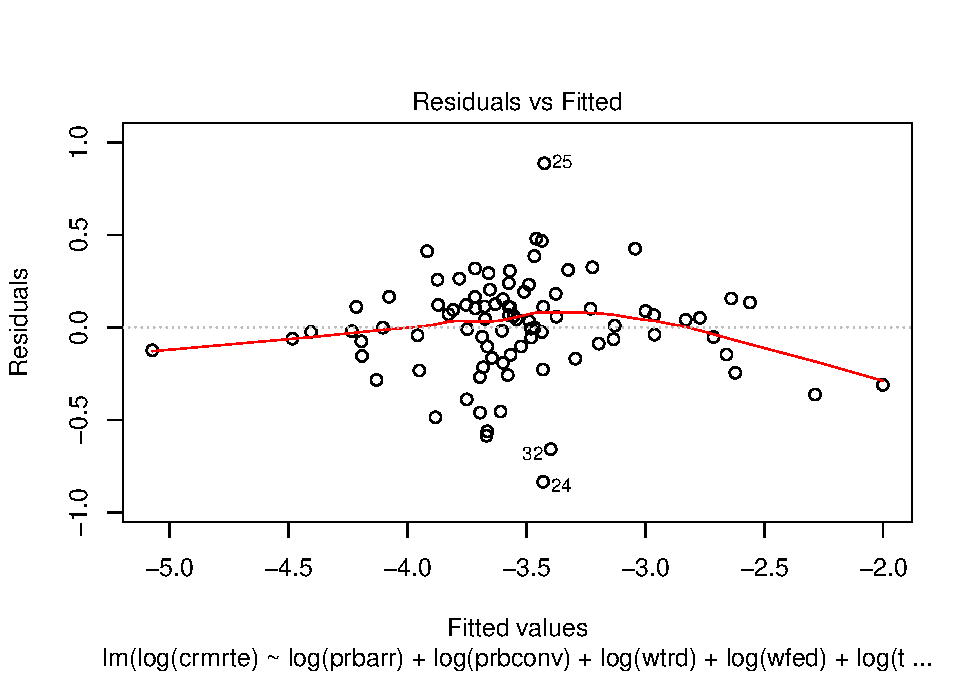
\includegraphics{lab_3_final_files/figure-latex/unnamed-chunk-47-1} 

}

\caption{Figure 15}\label{fig:unnamed-chunk-47}
\end{figure}

Notice that there is only a slight deviation from zero conditional mean,
indicated by a not perfectly flat curve. This means that our
coefficients maybe be biased. In the next section, we discuss some
omitted variables candidates and the bias direction they would imply.

\hypertarget{homoskedasticity}{%
\subsubsection{Homoskedasticity}\label{homoskedasticity}}

Our residuals versus fitted values plot seems to indicate
heteroskedasticity based on the scale location plot. We see a bump for
values close to the mean and high end of the distribution.

\begin{Shaded}
\begin{Highlighting}[]
\KeywordTok{plot}\NormalTok{(mod3, }\DataTypeTok{which =} \DecValTok{3}\NormalTok{)}
\end{Highlighting}
\end{Shaded}

\begin{figure}

{\centering 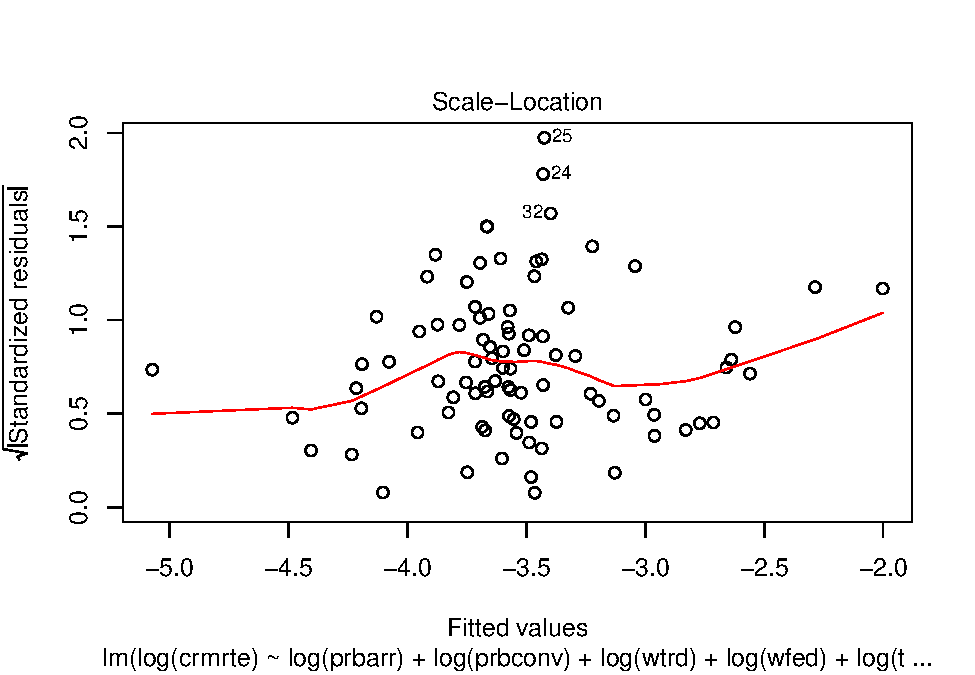
\includegraphics{lab_3_final_files/figure-latex/unnamed-chunk-48-1} 

}

\caption{Figure 16}\label{fig:unnamed-chunk-48}
\end{figure}

We used robust standard error to evaluate all our models, which is the
indicated strategy for dealing with heteroskedasticity.

\hypertarget{normality-of-errors}{%
\subsubsection{Normality of Errors}\label{normality-of-errors}}

To check normality of errors, we can look at the qqplot that's part of
R's standard diagnostics.

\begin{Shaded}
\begin{Highlighting}[]
\KeywordTok{plot}\NormalTok{(mod3, }\DataTypeTok{which =} \DecValTok{2}\NormalTok{)}
\end{Highlighting}
\end{Shaded}

\begin{figure}

{\centering 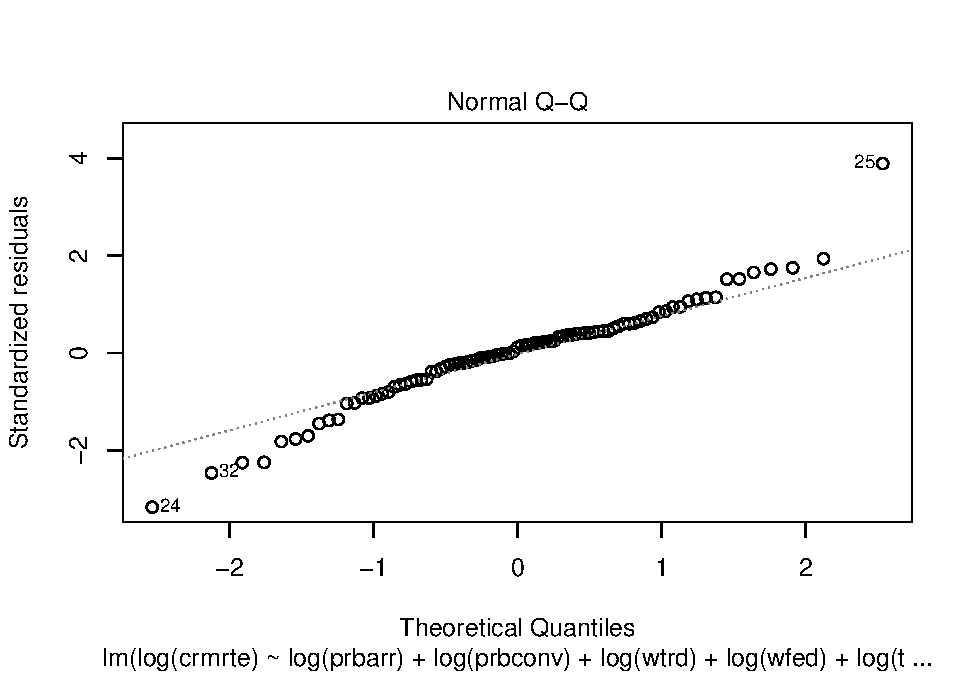
\includegraphics{lab_3_final_files/figure-latex/unnamed-chunk-49-1} 

}

\caption{Figure 17}\label{fig:unnamed-chunk-49}
\end{figure}

We can also visually look at the residuals directly.

\begin{Shaded}
\begin{Highlighting}[]
\KeywordTok{hist}\NormalTok{(mod3}\OperatorTok{$}\NormalTok{residuals, }\DataTypeTok{breaks =} \DecValTok{20}\NormalTok{, }\DataTypeTok{main =} \StringTok{"Residuals from Linear Model Predicting log(Crime Rate)"}\NormalTok{)}
\end{Highlighting}
\end{Shaded}

\begin{figure}

{\centering 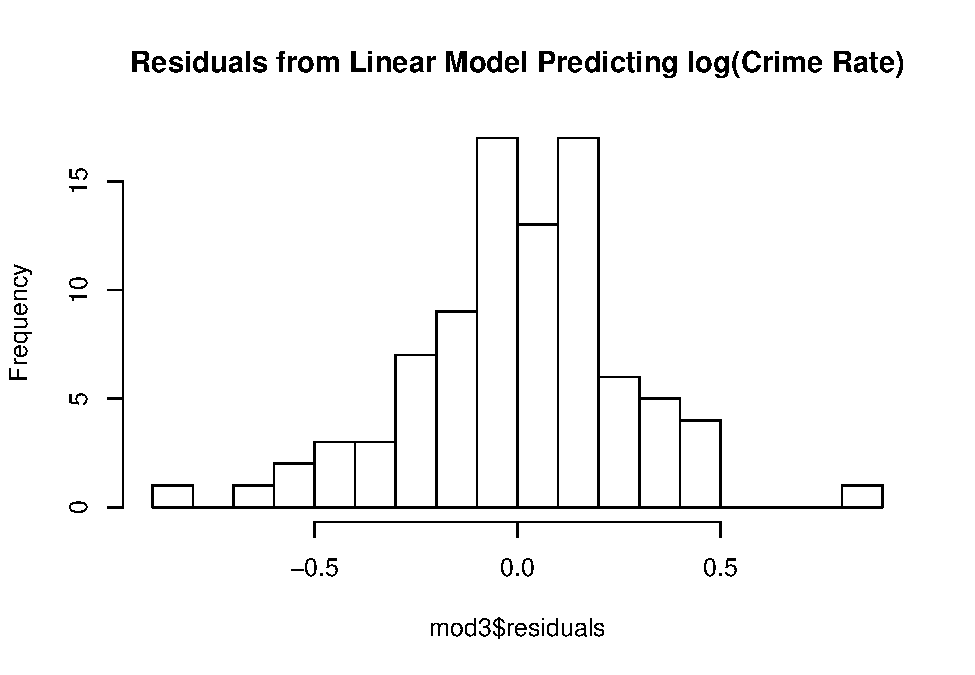
\includegraphics{lab_3_final_files/figure-latex/unnamed-chunk-50-1} 

}

\caption{Figure 18}\label{fig:unnamed-chunk-50}
\end{figure}

Both methods suggest we have a leftward skew. However, we have a large
sample size, so the CLT tells us that our estimators will have a normal
sampling distribution. The histogram confirms that we aren't in a
situation with an extreme skew, so n=90 should be sufficient for the
CLT.

\hypertarget{discussion-of-possible-omitted-variables-ov}{%
\section{Discussion of Possible Omitted Variables
(OV)}\label{discussion-of-possible-omitted-variables-ov}}

As discussed throughout the text - and hinted by ``Residual vs Fitted''
and ``Scale-Location'' plots - we have reason to believe that we lack
many variables that we expect relate to crime and can affect the
quantification of the relationships estimated above.

In order to access the direction of omitted variable bias (OVB) on the
estimated coefficients of criminal justice system variables resulting
from each of the OV, we analyze the product of two correlations:

\begin{itemize}
\tightlist
\item
  \(\alpha\) = correlation between the omitted variable and
  \texttt{crmrte}
\item
  \(\beta_2\) = correlation between the omitted variable and
  \texttt{prbarr}/\texttt{prbconv}
\end{itemize}

As we assume the true relationship between \texttt{crmrte} and
\texttt{prbarr}/\texttt{prbconv} (\(\beta_1\)) is negative, a positive
OVB biases the estimated effect of \texttt{prbarr}/\texttt{prbconv} on
\texttt{crmrte} towards zero, while a negative OVB biases the estimated
effect away from zero.

\textbf{Unemployment} (\(\alpha > 0\) and \(\beta_2 > 0\)
-\textgreater{} towards zero)

Unemployment rate is likely positively related to crime rate (so
\(\alpha > 0\)), people in need are more prone to commit crimes.
Unemployment rate is also arguably positively related to
\texttt{prbarr}/\texttt{prbconv} (so \(\beta_2 > 0\)) due to the
negative stigma that unemployment people have in society. Thus this OV
should bias the estimated effect of \texttt{prbarr}/\texttt{prbconv} on
\texttt{crmrte} away from zero.

\textbf{Education levels of the populace} (\(\alpha < 0\) and
\(\beta_2 < 0\) -\textgreater{} towards zero)

Although we may be able to proxy education levels by looking at which
region a county is in, we would not have a very good measure of overall
education levels. A county can have a university, but still have low
education levels overall. One would predict that education is negatively
related to crime - the more educated, the less crime one would expect to
commit (so \(\alpha < 0\)). The relationship between education levels
and \texttt{prbarr}/\texttt{prbconv} is arguably negative due to the
negative stigma that less educated people have in society (so
\(\beta_2 < 0\)).

\textbf{Public works \& investments} (\(\alpha < 0\) and \(\beta_2 < 0\)
-\textgreater{} towards zero)

One would predict that the relationship between and public works and
investments with crime would be negative (so \(\alpha < 0\)). More
nonprofits and community organizations could strengthen ties in
communities, thus lowering crime rates. This factor would probably be
inversely related to arrest and conviction rates, since a more punitive
society may invest less in rewards to the community (so
\(\beta_2 < 0\)).

\textbf{Individual Health (mental and physical)} (\(\alpha < 0\) and
\(\beta_2 < 0\) -\textgreater{} towards zero)

Health - mental and physical - would likely be related to less crime.
The healthier you are, the more mental and physical resources you have
to solve problems in ways that do not necessitate committing a crime (so
\(\alpha < 0\)). The direction of the relationship to arrest or
conviction rates is fuzzier but one could imagine that communities that
have a focus on health may tend to be less punitive (so
\(\beta_2 < 0\)).

\textbf{Community Health} (\(\alpha < 0\) and \(\beta_2 < 0\)
-\textgreater{} towards zero)

Community health is about the cohesiveness of a community. If you have
good supports in your community, you would be less likely to commit
crime (so \(\alpha < 0\)). This factor would probably be inversely
related to arrest and conviction rates, since a more loving, cohesive
community may be less likely to turn to punishment (so \(\beta_2 < 0\)).

\textbf{Inequality} (\(\alpha > 0\) and \(\beta_2 < 0\) -\textgreater{}
away from zero)

With more inequality, one would expect to see more crime - more anger
and therefore reasons to commit crime combined with greater levels of
deprivation and need to commit crime would naturally lead to more crime
(so \(\alpha > 0\)). A more egalitarian society may have less punitive
practice, since people would see each other as closer to their own
group. This can help humanize other people and make it harder to commit
cruelties (so \(\beta_2 < 0\)).

We cannot exactly determine the size of each of the biases above,
however since most of them are in the same direction the net effect
likely has led us to underestimate the (negative) relationship between
crime rate and these criminal justice policies.

\emph{What about our economic policy variables?} Assuming that
\texttt{wtrd} is a good proxy for minimum wage, omitted variables could
have caused the coefficient on \texttt{wtrd} to not be significant
across our models. Recall that, as we assume the true relationship
between \texttt{crmrte} and minimum wage is negative, a positive OVB
biases the estimated effect of \texttt{wtrd} on \texttt{crmrte} towards
zero, while a negative OVB biases the estimated effect away from zero.

The unemployment rate is an important candidate of OV that can be
biasing the estimated effect of \texttt{wtrd} on \texttt{crmrte}
\emph{towards zero}. As argued above, the unemployment rate is likely
positively related to crime rate, as people in need are more prone to
commit crimes. Meanwhile, even though there has been mixed evidence
around increases in minimum wage and unemployment, the consensus - as
per this
\href{https://journals.sagepub.com/doi/abs/10.1177/001979399204600105}{article}
- is that unemployment and minimum wage increases are positively
correlated, so we will make that assumption here. Thus, including an
unemployment variable could increase the estimated impact of economic
policy. We cannot determine the size of this relationship but since
evidence is mixed we would guess that it would be a medium impact.

\hypertarget{conclusion-3}{%
\section{Conclusion}\label{conclusion-3}}

Our analyses suggest that acting on crime deterrents within the criminal
justice system (like arrests and convictions) is an important policy
target for preventing crime. In fact, for a 10\% rise in the probability
of arrests and convictions individually, the negative impact on crime
rate hovers between 4-7\% for the arrests and between 3-5\% for
convictions. Helpful follow-ups to this investigation would be to
leverage variation across time and possibly test for large changes in
policy that, for example, would help in designing a regression
discontinuity model. However, our findings can be used to hone in on
future policy changes that can be evaluated with more rigorous causal
analyses.

Most of the omitted variables we considered as potentially biasing the
estimated effect of arrests and convictions rates on crime rate would
cause a bias towards zero - i.e., including them in the model would
likely lead to an even stronger estimated coefficient of arrests and
convictions rates in our crime model. This finding made us more
confident about the call that politicians could leverage criminal
justice policies to curb crime rate.

On the other hand, we could not find much support for the importance of
economic policy variables to prevent crimes. In the absence of a better
measure, we used average wages in the trade industry as a proxy for a
minimum wage and found no statistically significant impact of this wage
on crime. We argued that there are omitted factors (such as the
unemployment rate) that would likely bias the estimated coefficient of
average wage towards zero.

Real life variations in these counties lead to some extreme values - we
did not remove these, as they were likely edge cases rather than
erroneous data. Any policies should take the local context into
consideration for these extreme cases. A stronger follow-up study would
control for more of these within-county factors to produce more robust
causal findings. The distribution of minorities is a good example of one
of these important contextual variable that is not (at least ethically)
under the influence of a politician. Communities with higher rates of
minorities or crime may require additional resources or different types
of policies to prevent crime. For example, if the actual number of
crimes is different from the number of reported crimes - in a community
with a lot of racial conflict some groups over-report others to the
police - we would see elevated measures of crime. If policies aim to
reduce actual crime, we would need more nuanced measures to track and
address this crime issue (e.g., hosting workshops to reduce racism).

In conclusion, we recommend policies that increase arrests and
convictions alongside those that help increase the cost of living in an
area. However, further analysis with the inclusion of omitted variables
is needed to guarantee the actual impact on crime rate of changing these
factors. An important tactic for any politician would be to fund
research that can more rigorously tease out these causal factors.


\end{document}
